\documentclass[a4paper,11pt,twoside]{article}
\usepackage[utf8]{inputenc}	% Text coding
\usepackage[T1]{fontenc}
\usepackage{lmodern}
\usepackage[czech]{babel}
\usepackage{epsfig}
\usepackage{amsfonts,amsmath,amssymb}
\usepackage{graphicx}
\usepackage[unicode]{hyperref}
\usepackage{indentfirst}
\usepackage{fancyhdr}
\usepackage{xifthen}
\usepackage{amsthm,thmtools}
\usepackage{bold-extra}
\usepackage[dvipsnames]{xcolor}
\usepackage[subrefformat=simple,labelformat=simple]{subcaption} % Instead of subfigure
\usepackage{listings}
\usepackage{comment}
\usepackage{titlesec}
\usepackage{underscore}
\usepackage{makecell}       % Šířky čar v tabulkách
\usepackage{fnpct}          % %% Lepší formátování poznámek pod čarou 
%\usepackage{showlabels}

\hypersetup{
	pdftitle={Využití počítačů ve fyzice},
	pdfauthor={Pavel Stránský},
	pdffitwindow=true,
	colorlinks=true,
	urlcolor=cyan,
	linkcolor=red,
	citecolor=green,
	filecolor=magenta
}

\graphicspath{{figures/}}

\lstdefinestyle{listingsstyle}{
    basicstyle=\ttfamily,
    breakatwhitespace=false,         
    numbersep=3,
    breaklines=true,                 
    keepspaces=true,                 
    showspaces=false,                
    showstringspaces=false,
    showtabs=false,                  
    tabsize=2,
    columns=fullflexible,
}

\lstset{style=listingsstyle}

\lstdefinestyle{TinyPython}{
    language=Python,
    basicstyle=\normalfont\ttfamily\footnotesize
}

\lstdefinestyle{NormalPython}{
    language=Python,
    basicstyle=\normalfont\ttfamily
}

\lstdefinestyle{console}{
    basicstyle=\ttfamily\footnotesize\color{white},
    backgroundcolor=\color{black}
}

%\babelhyphenation[czech]{ma-te-ma-tic-kých}

\renewcommand\thesubfigure{(\alph{subfigure})}

\newcommand{\subsubsubsection}[1]{\paragraph{#1}\mbox{}

}

\setcounter{secnumdepth}{5}
\setcounter{tocdepth}{5}

% Page size
\addtolength{\topmargin}{-1.5cm} %\addtolength{\textheight}{-10cm}
\addtolength{\textwidth}{4cm} \addtolength{\textheight}{4cm} % Width and height of the text
\addtolength{\voffset}{-0.5cm} % Top margin
\addtolength{\hoffset}{-2cm}
\setlength{\headheight}{15pt}

\pagestyle{fancy}

\DeclareMathOperator{\e}{e}

\def\vector#1{\boldsymbol{#1}}								% Vector
\renewcommand{\d}{\mathrm{d}}
\newcommand{\derivative}[3][]{\ifthenelse{\isempty{#1}}	    % Normal derivative
	{\frac{\d{#2}}{\d{#3}}}
	{\frac{\d^{#1}{#2}}{\d{#3}^{#1}}}
}
\newcommand{\im}{\mathrm{i}}

\def\makematrix#1{\begin{pmatrix}#1\end{pmatrix}}       % Matrix
\def\abs#1{\left|#1\right|}
\def\probability#1{\mathrm{Pr}\left[#1\right]}
\def\expectation#1{\mathrm{E}\left[#1\right]}
\def\dispersion#1{\sigma_{#1}^{2}}

\def\code#1{\textnormal{\texttt{#1}}}
\def\file#1{\textnormal{\textbf{\texttt{#1}}}}
\def\ghfile#1#2{\textnormal{\textbf{\texttt{\href{https://github.com/PavelStransky/PCInPhysics/blob/main/#1#2}{#2}}}}}

\def\abbreviation#1{\textnormal{\textsc{#1}}}

\long\def\python#1{{\color{ForestGreen}#1}}

\newtheoremstyle{spaced}
{5pt}{5pt}{\itshape}{}{\bfseries}{:}{.5em}{}

\newtheoremstyle{red}
{5pt}{5pt}{\itshape\color{red}}{}{\bfseries\color{red}}{:}{.5em}{}

\newtheoremstyle{green}
{5pt}{5pt}{\itshape\color{ForestGreen}}{}{\bfseries\color{ForestGreen}}{:}{.5em}{}

\newtheoremstyle{blue}
{5pt}{5pt}{\itshape\color{blue}}{}{\bfseries\color{blue}}{:}{.5em}{}

\theoremstyle{red}
\declaretheorem[name=Úkol,numberwithin=section]{task}

\theoremstyle{green}
\declaretheorem[name=Úkol,numberwithin=section,sibling=task]{voluntary}

\begin{document}

\theoremstyle{spaced}
\newtheorem{example}{Příklad}[section]

\theoremstyle{blue}
\newtheorem{solution}{Řešení}[section]

\title{Poznámky k předmětu Využití počítačů ve fyzice}
\date{\today}
\author{Pavel Stránský}

\maketitle
\tableofcontents

\newcommand{\sectionbreak}{\clearpage}

\section{Úvod}
\label{sec:Uvod}
    Cílem tohoto cvičení je pohrát si s jednoduchými fyzikálními problémy, vyzkoušet si různé způsoby jejich řešení a získat {\bf zkušenost a odvahu} pro řešení složitějších problémů v budoucnosti.
    Postupy a kódy, které si budeme ukazovat, nemusejí být ty nejsofistikovanější či nejoptimálnější.
    Půjde nám hlavně o srozumitelnost a o pochopení principu, jak nejběžnější numerické algoritmy fungují, jaký algoritmus zvolit pro konkrétní úlohu, jaké mají probírané algoritmy vlastnosti a na co si při jejich použití dát pozor.
    Vzhledem k tomu, že prezentované algoritmy budou relativně jednoduché, budeme se snažit o maximální eleganci výsledného programu, přičemž pod elegancí budeme chápat hlavně dobrou {\bf čitelnost a udržitelnost} kódu.
    
    Ve cvičení nebude probíhat systematická výuka žádného programovacího jazyka ani numerických algoritmů, k tomu slouží jiné dedikované přednášky.
    Od účastníka cvičení se očekává, že již prošel kurzem základů programování a je schopen napsat funkční kód v nějakém aktuálním programovacím jazyce.

    \subsection{Výběr programovacího jazyka}
        Většina příkladů cvičení bude demonstrována v programovacím jazyce \href{https://python.org}{Python}.
        Jeho výhodou je jednoduchost, v dnešní době velká rozšířenost a existence nepřeberného množství pokročilých knihoven, které lze snadno použít.
        Neznamená to, že se musíte upínat k Pythonu, pokud vám není sympatický nebo pokud ovládáte jiný programovací jazyk a chcete raději pilovat své schopnosti v něm.
        Každé cvičení bude mít vždy \uv{teoretickou část}, ve které budou algoritmy a techniky vysvětleny bez vazby na konkrétní programovací jazyk.
        Výsledné programy pak nebudou nijak obsáhlé a až na výjimky (úvod do paralelizace) nebudou vyžadovat při programování žádné speciální finesy,\footnote{Například objektově orientované programování, abstraktní typy, asynchronní programování atd.}
        lze je tudíž napsat snad v jakémkoliv dnes používaném jazyce.
        Pokud se rozhodnete (nyní nebo kdykoliv v budoucnu) pro jiný jazyk než Python, doporučuji dát si pozor na následujících několik bodů, ve kterých se programovací jazyky lišívají:
        \begin{itemize}
            \item \emph{Indexování:} Některé programovací jazyky indexují pole od 0, jiné od 1. Ve dvou a vícerozměrných polích může první index udávat někdy řádek, jindy sloupec.
            \item \emph{Číselné typy a implicitní přetypování:} Rozdíly jsou zejména u operace dělení / dvou celých čísel, kde v některých jazycích je výsledkem celé číslo, tedy celá část po výsledku dělení, v jiných číslo s destinnou čárkou.
            Různě také funguje implicitní přetypování, a to zejména mezi číslem a řetězcem (výrazy typu \code{"12.3"{} + 4}).
            \item \emph{Parametry funkcí} mohou být předávané hodnotou nebo odkazem. 
            Pokud jsou předávané odkazem, pak při změně hodnoty proměnné uvnitř funkce dojde ke změně i vně funkce.
            Podobně může fungovat přiřazení jedné proměnné do druhé.
            \item \emph{Obor platnosti proměnných:} Některé programovací jazyky mají bloky, ve kterých pokud deklarujeme proměnnou, při opuštění bloku přestane být dostupná.
            V jiných jazycích může být obor platnosti proměnné například celá funkce.
            V některých jazycích neexistují globální proměnné.\footnote{I pokud existují, doporučuje se jejich použití omezit na minimum a používat je jen v opravdu odůvodněných případech.}
            \item \emph{Správa paměti:} Drtivá většina dnešních programovacích jazyků má automatickou správu paměti, kdy nemusíte řešit, kdy a kolik paměti alokujete a že ji musíte uvolnit, když ji přestanete používat.
            Nízkoúrovňové jazyky (například C/C++) však vyžadují, aby se o správu paměti staral programátor sám.
        \end{itemize}

        Pro fyzika je navíc důležité, aby programovací jazyk, který si zvolí, byl silný v následujících bodech:
        \begin{itemize}
            \item \emph{Existence základních numerických knihoven:} Nejčastěji je potřeba numerické řešení diferenciálních rovnic, práce s pseudonáhodnými čísly, diagonalizace matic a fitování parametrů funkcí ze zadaných dat.
            Užitečná je také rychlá Fourierova transformace a v dnešní době i možnost zvýšení přesnosti čísel s desetinnou čárkou nad standardních 64-bitů.
            Experimentátoři využijí pokročilé možnosti analýzy a filtrování dat.
            \item \emph{Možnost tvorby grafů:} Grafická reprezentace výsledků bývá obvykle nejčitelnější a nejsrozumitelnější. 
            V základu se hodí grafy funkcí s jedním parametrem a konturové grafy.
            V dnešní době je navíc výhodou, pokud program umí vytvořit animace.
            \item \emph{Možnost spustit program na různých platformách:} Výpočetní clustery a dedikované výpočetní počítače pracují často pod jinými operačními systémy než běžné osobní počítače.
            Programovací jazyk by měl existovat a být snadno nainstalovatelný zejména na stroje s operačním systémem Linux.
            \item \emph{Podpora distribuovaných výpočtů a výpočtů ve více vláknech:} Výpočetní síla dnešních počítačů používaných ve vědě spočívá v paralelizaci. 
        \end{itemize}

    \subsection{Výběr vývojového prostředí}
    \label{sec:IDE}
        Zatímco na volbě programovacího jazyka záleží, co všechno budeme schopni naprogramovat a jak budou výsledné programy rychlé a efektivní, tak to, jak se nám bude dobře a rychle kód psát, záleží na volbě vývojového prostředí.
        Na funkčnost výsledného programu nemá vliv, zda jsme ho napsali v jednoduchém textovém editoru nebo v sofistikovaném programu s pokročilými možnostmi spouštění, ladění a verzování kódu.
        Je ale jasné, že to druhé nám významně usnadní práci a sníží pravděpodobnost chyb, které náš program bude nakonec obsahovat.

        Jako vývojové prostředí v tomto cvičení bude používáno \href{https://code.visualstudio.com/}{Visual Studio Code}.
        Tento volně dostupný program lze nainstalovat na všechny neužívanější operační systémy (Linux, Windows, MacOS).    
        Má nepřeberné možnosti při editaci zdrojových souborů, překladu a ladění snad ve všech známých programovacích jazycích.
        Bohaté možnosti nastavení umožnují přizpůsobit si práci svým potřebám (například zvýrazňování syntaxe, klávesové zkratky či vzhled prostředí).
        Pomocí doplňků ho můžete integrovat s dalšími službami, například s verzovacím programem Git nebo vzdálenými repozitáři, čehož také využijeme.
        Komunita, která toto vývojové prostředí používá a spravuje, je obrovská, což zaručuje dobrou podporu a rychlé přidávání nových funkcí.
        Je to právě univerzálnost a rozšířenost tohoto vývojového prostředí, díky které padla volba na něj.
        
        Pro Python existuje samozřejmě obrovské množství dalších velmi kvalitních vývojových prostředí. 
        Nejčastěji používané jsou
        \begin{itemize}
            \item \abbreviation{\href{https://docs.python.org/3/library/idle.html}{IDLE}}:\footnote{
                {\bf I}ntegrated {\bf D}evelopment and {\bf L}earning {\bf E}nvironment.
            } 
                Toto jednoduché vývojové prostředí je součástí instalace jazyka Python.
                Obsahuje základní zvýrazňování syntaxe, má však omezené možnosti co se týče ladění, psaní rozsáhlejších projektů s více zdrojovými soubory nebo integrace s verzovacími programy.
            \item \href{https://www.spyder-ide.org/}{Spyder} a \href{https://www.jetbrains.com/pycharm/}{PyCharm}:
                Vývojová prostředí s pokročilými funkcemi přímo určená pro jazyk Python.
                Vynikající alternativy pro Visual Studio Code, které v mnoha ohledech dokonce překonávají.
            
            \item \href{https://jupyter.org/}{Jupyter}: 
                Jiná koncepce práce s programovacím jazykem.
                Kód je součástí tzv. \emph{zápisníku (notebook)}, ve kterém může být zároveň strukturovaný a formátovaný text.\footnote{Stejný přístup má například program \href{https://www.wolfram.com/mathematica/}{Mathematica}, které se budeme věnovat v sekci~\ref{sec:Mathematica}.}
                Jedná se tedy o kombinaci programu a poznámek, kde součástí poznámek jsou přímo výsledky výpočtů (tabulky, grafy atd.).
                Zápisník lze snadno konvertovat například do formátu LaTeX nebo PDF.
                Koncepce zápisníku však není příliš vhodná při použití verzovacích programů a při práci na rozsáhlejších projektech v týmu.
        \end{itemize}

        Pokud teprve vybíráte, které vývojové prostředí se naučíte, doporučuji zvážit, zda potřebujete následující funkce a vlastnosti a nakolik je dané vývojové prostředí podporuje.

        \begin{itemize}
            \item \emph{Zvýrazňování syntaxe:} Pomáhá čitelnosti a snazží orientaci v kódu.
            \item \emph{Spouštění a ladění kódu (debugger):} To zahrnuje vkládání \emph{ladících bodů (breakpoints)}, na kterých se chceme, aby se program zastavil, možnost krokování a výpisu (a často i editace) aktuálních hodnot proměnných či podrobné informace o chybách, pokud k nim při provádění programu dojde, včetně rychlého skoku na příslušná místa kódu.
            \item \emph{Našeptávání a automatické doplňování:} Zatímco dříve byly názvy proměnných často omezené na malý počet znaků, dnešní programovací jazyky umožňují používat v podstatě libovolnou délku. Není také nutné omezovat se jen na znaky ASCII, nýbrž proměnné a funkce lze pojmenovávat včetně symbolů s diakritikou a písmen z jiných abeced (včetně například řeckých písmen). Klidně delší, ale výstižné pojmenování proměnných se doporučuje i kvůli lepší čitelnosti kódu bez nutnosti obsáhlých a na údržbu náročných komentářů. Automatické dokončování výrazně zrychluje psaní a snižuje množství chyb a překlepů.
            \item \emph{Integrace s verzovacími systémy:} Pokud budete pracovat na větším týmovém projektu, použití verzovacích systémů se nevyhnete. Práci usnadňuje, když samotné vývojové prostředí umí zapisovat nové verze a porovnávat různé verze téhož souboru s vyznačením provedených změn.
        \end{itemize}

\section{Instalace používaných nástrojů}
\label{sec:Instalace}
    Vzorové příklady k cvičení budou vypracovány v nejnovější verzi programovacího jazyka \href{https://python.org}{Python}.
    Jako vývojové prostředí bude používáno \href{https://code.visualstudio.com}{Visual Studio Code}.
    V této sekci si stručně ukážeme, jak programy nainstalovat a jak provést jejich základní nastavení.

\subsection{Instalace Pythonu}
\label{sec:InstalacePython}
    Instalační soubor pro svůj operační systém stáhnete ze stránky \url{https://www.python.org/downloads/}.
    Při instalaci na počítač s Windows doporučuji zvolit \uv{Add Python to PATH}, což zjednoduší práci s Pythonem z příkazové řádky, a na posledním dialogovém okně obrazovce zvolit \uv{Disable path length limit} (pokud je tato volba k dispozici):
    \begin{center}
        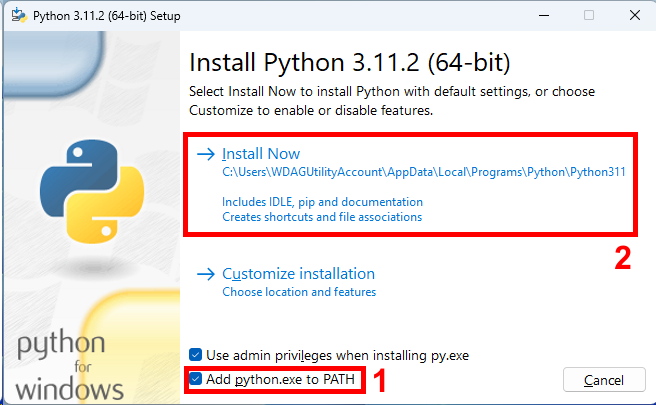
\includegraphics[width=0.495\linewidth]{PythonInstallPath.png}
        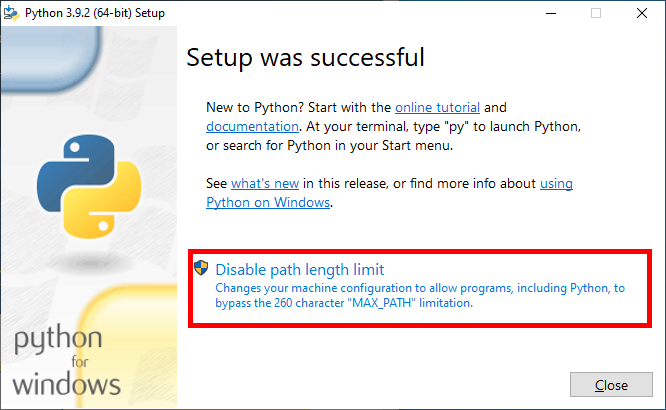
\includegraphics[width=0.495\linewidth]{PythonInstallPathLimit.png}
    \end{center}
    Pro ověření instalace napíšeme v příkazové řádce příkaz \code{python}.\footnote{Na počítačích s Linuxem je příkaz v terminálu \code{python3}.}
    Tím se spustí \abbreviation{REPL}\footnote{{\bf R}ead-{\bf E}valuate-{\bf P}rint-{\bf L}oop.} Pythonu, ve které můžeme již psát všechny příkazy programovacího jazyka, které se po zadání ihned provedou a vypíšou výsledek.
    REPL ukončíme zadáním příkazu \code{exit()}.

\subsubsection{Instalace doplňujících knihoven}
\label{sec:pip}
    Samotná instalace Pythonu obsahuje jen minimální množství nejnutnějších knihoven.
    My budeme využívat ještě následující rozšiřující knihovny:
    \begin{itemize}
        \item \file{\href{https://numpy.org}{NumPy}} ({\bf Num}erical {\bf Py}thon: numerická matematika, řady a vícedimenzionální datové typy),
        \item \file{\href{https://scipy.org}{SciPy}} ({\bf Sci}entific {\bf Py}thon: algoritmy pro optimalizaci, statistiku, řešení diferenciálních rovnic, lineární algebru, atd.),
        \item \file{\href{https://matplotlib.org}{Matplotlib}} (vizualizace, grafy).
    \end{itemize}
    K jejich doinstalování slouží modul \code{pip}.
    V příkazové řádce napíšeme
    \begin{lstlisting}
        python -m pip install numpy scipy matplotlib\end{lstlisting}
    čímž se nainstalují naráz všechny tři knihovny.\footnote{
        Pokud na počítači s Linuxem uvedený postup nebude fungovat, je potřeba nejprve nainstalovat instalátor \file{pip} pomocí příkazu \code{sudo apt install python3-pip}.
        Pak lze použít buď výše uvedený příkaz, nebo stručnější \code{pip3 install numpy}.
    }
    
    Existuje samozřejmě celá řada dalších užitečných a používaných knihoven, jako je například 
    \begin{itemize}
        \item \file{\href{https://pandas.pydata.org/}{Pandas}} pro zpracování a analýzu dat,
        \item \file{\href{https://www.sympy.org/}{SymPy}} pro symbolické výpočty,
        \item \file{\href{https://www.tensorflow.org/}{TensorFlow}}, 
            \file{\href{https://scikit-learn.org}{scikit-learn}} (a další) pro strojové učení,
        \item \file{\href{https://qutip.org/}{QuTiP}} pro simulace kvantových systémů,
    \end{itemize} 
    a nepřeberné množství vysoce specializovaných knihoven pro konkrétní fyzikální, matematické či statistické úkoly.
    S nimi se seznámíte ve specializovaných kurzech a přednáškách.

\subsection{Instalace Visual Studio Code}
    Zde projdeme instalaci vývojového prostředí \href{https://code.visualstudio.com}{Visual Studio Code} s doplňkem pro programovací jazyk Python.
    Instalační soubor stáhnete ze stránky \url{https://code.visualstudio.com}.
    Během instalace na počítač s Windows doporučuji zvolit obě možnosti \uv{Add Open with Code action to...},
    \begin{center}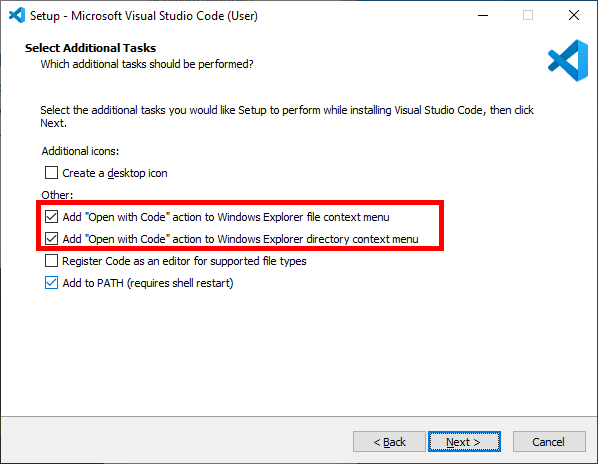
\includegraphics[width=0.5\linewidth]{VSCodeInstall.png}\end{center}
    což zjednoduší otevírání složek s projekty nebo samostatných souborů pomocí pravého tlačítka myši.

    Na operačním systému Linux je nejjednodušší provést instalci pomocí Snap Store příkazem v terminálu
    \begin{lstlisting}
        sudo snap install --classic code\end{lstlisting}
    nebo použít tento \href{https://code.visualstudio.com/docs/setup/linux}{návod}.
    
    \subsubsection{Klávesové zkratky}
    Ačkoliv veškeré funkce vývojového prostředí Visual Studio Code lze používat pomocí myši, pro seriózní práci je dobré se naučit klávesové zkratky, jelikož významně zrychují a zefektivňují práci.
    Základní klávesové zkratky (nový soubor, uložení souboru, hledání v souboru, navigace v souboru, kopírování a vkládání atd.) fungují stejně jako v jiných programech.
    Kromě toho je ve Visual Studiu Code množství klávesových zkratek, které usnadňují editaci, spouštění, ladění a správu kódu.
    Všechny klávesové zkratky lze zobrazit a upravit podle vlastních preferencí postupným stiskem kláves \code{Ctrl+K Ctrl+S}.

    Klávesové zkratky se liší podle použitého operačního systému.
    Doporučuji vám projít si oficiální \uv{taháky} s nejdůležitějšími zkratkami pro
    \href{https://code.visualstudio.com/shortcuts/keyboard-shortcuts-windows.pdf}{Windows}, 
    \href{https://code.visualstudio.com/shortcuts/keyboard-shortcuts-linux.pdf}{Linux} i 
    \href{https://code.visualstudio.com/shortcuts/keyboard-shortcuts-macos.pdf}{MacOS} 
    přímo od tvůrců tohoto vývojového prostředí.
    Uvedené klávesove zkratky platí pro rozložení klávesnice Angličtina (Spojené státy).
    Pro jiné rozložení klávesnice nemusejí některé z nich fungovat.

    Pro operační systém Windows nejdůležitější zkratky jsou:
    \begin{itemize}
        \item \code{Alt+Z}: Zalomí dlouhé řádky na konci okna.
        \item \code{Alt+←}: Vrátí kurzor na předchozí pozici (například po odskrolování někam do neznáma).
        \item \code{Ctrl+/}: Přidá či odstraní komentář řádku.
        \item \code{Ctrl+[, Tab}: Odsadí označenou část kódu o jednu úroveň.
        \item \code{Ctrl+], Shift+Tab}: Zmenší odsazení označené části kódu o jednu úroveň.
        \item \code{Ctrl+Mezera}: Zobrazí okénko s nápovědou k danému symbolu.
        \item \code{F12}: Posune kurzor na definici daného symbolu (proměnné, funkce, atd.).
        \item \code{Shift+F12}: Zobrazí všechny reference na daný symbol.
        \item \code{Ctrl+G}: Přechod na řádek s daným číslem.
        \item \code{Ctrl+Shift+O}: Zobrazí všechny definované symboly v otevřeném okně.
        \item \code{F2}: Přejmenuje symbol (proměnnou, funkci, atd.) v rozahu jeho platnosti.
        \item \code{Shift+Enter}: Spustí označenou část kódu v konzoli.
        \item \code{Ctrl+F5}: Spustí otevřený soubor.
        \item \code{F5}: Spustí otevřený soubor v režimu ladění.
        \item \code{F9}: Přidá ladící bod.
    \end{itemize}


\subsubsection{Instalace doplňku pro Python}
    \begin{center}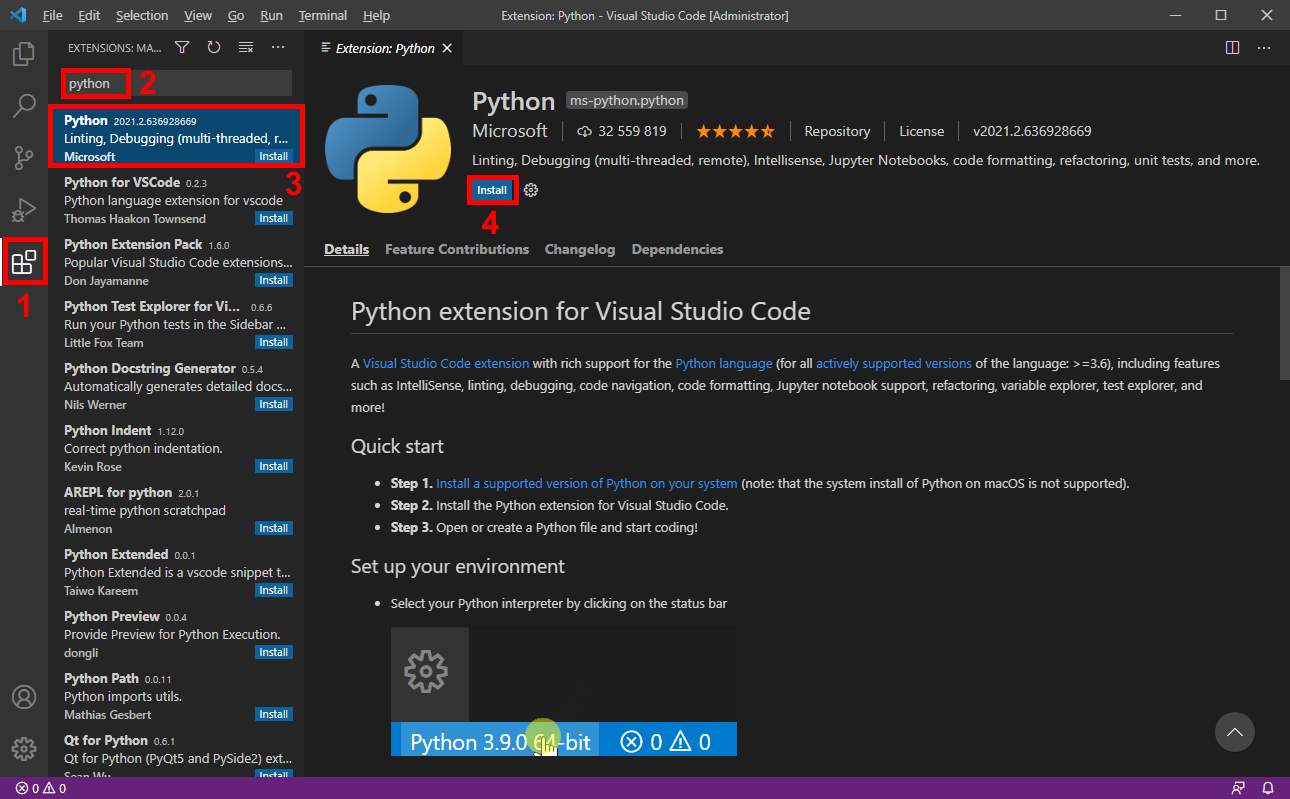
\includegraphics[width=\linewidth]{VSCodeInstallPython.png}\end{center}
    Ke správě doplňků (extensions) se dostanete kliknutím na ikonku {\color{red} 1} nebo stisknutím \code{Ctrl+Shift+X}. 
    Vyhledáte doplněk \href{https://marketplace.visualstudio.com/items?itemName=ms-python.python}{Python} {\color{red} 2} od Microsoftu, vyberete ho {\color{red} 3} a nainstalujete {\color{red} 4}.

\subsection{Instalace Git}
    Instalační soubor verzovacího systému \href{https://git-scm.com}{Git} stáhnete z webové stránky \url{https://git-scm.com}.
    K instalaci Gitu potřebujete administrátorská práva na svém počítači.
    
    V následujícím postupu zobrazuji jen ty snímky obrazovky, na kterých je vhodné vybrat jinou volbu, než jaká je instalátorem standardně nabízena.
    \begin{center}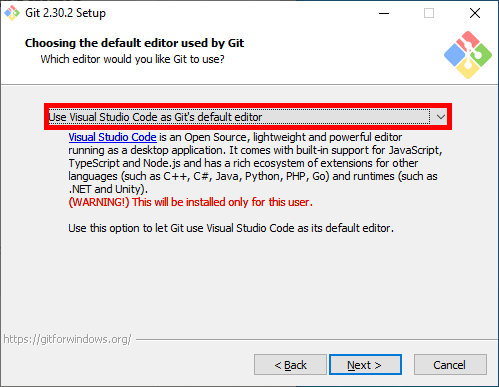
\includegraphics[width=0.5\linewidth]{GitInstallEditor.png}\end{center}
    Jako editor zvolíme dříve nainstalované Visual Studio Code.
    Systém Git vyžaduje editor jednak pro povinný komentář každé zapsané změny (commit), jednak pro ošetření kolizí při slučování větví (merge).
    \begin{center}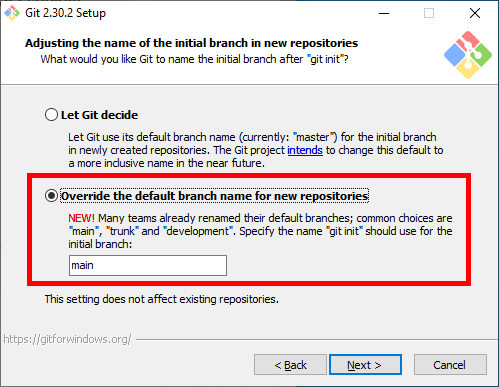
\includegraphics[width=0.5\linewidth]{GitInstallMain.png}\end{center}
    Hlavní větev repozitáře se donedávna standardně jmenovala \code{master}.
    Vzhledem k negativním konotacím tohoto slova v angličtině se přechází na neutrálnější označení.
    Nejběžnější je \code{main}, na které již přešel i populární správce vzdálených repozitářů \href{https://github.com}{GitHub}.
    Doporučuji tedy zvolit pojmenování \code{main}.

    Všechna ostatní nastavení, na která se táže instalační program, nechte na doporučené hodnotě. 
    Nastavení lze samozřejmě kdykoliv po instalaci změnit.

\subsection{Anaconda}
    Ačkoliv platforma \href{https://www.anaconda.com/}{Anaconda} nebude v tomto kurzu využívána, vzhledem k jejímu rozšíření stojí za to se o ní zmínit.
    Jedná se o rozsáhlý balík programů zahrnující instalaci Pythonu a velké množství knihoven včetně všech knihoven zmiňovaných v sekci~\ref{sec:pip}.
    Balík navíc obsahuje samostatnou instalaci vývojového prostředí Visual Studio Code a několik dalších vývojových prostředí včetně nejznámějších Spyder a Jupyter, které byly zmíněny v sekci~\ref{sec:IDE}.
    Výhoda platformy Anaconda a platforem podobného typu spočívá v tom, že všechny knihovny jsou vybrány s ohledem na to, aby byly mezi sebou kompatibilní a aby byly zároveň kompatibilní s použitou verzí Pythonu.
    To je však zároveň i hlavní nevýhodou: verze Pythonu a přiložených knihoven nikdy není ta nejaktuálnější dostupná na trhu, a tedy nelze používat nejnovější funkce a rysy jazyka.
    Navíc Anaconda bude vždy obsahovat množství knihoven a programů, které nevyužijete, jen budou zabírat místo na disku a mohou zpomalovat chod používaných funkcí.

\section{Úvod do používaných nástrojů}
    V této sekci naleznete základy použití verzovacího systému Git a úvod do syntaxe a idiomatiky jazyka Python.
    Tato sekce tvoří jakousi stručnou technickou \uv{referenční příručku}, ke které se budou následující části poznámek odkazovat.

\subsection{Verzovací systém Git}
    Každý si patrně už někdy v životě zasteskl, že nemá uložené dřívější verze svých souborů.
    Změny, které se ukazují být nevhodné či provedené omylem (kočka nepozorovaně přejde po klávesnici a my pak soubor uložíme), kamarád, který z nějakých důvodů chce zrovna tu verzi vašeho programu, kterou jste mu poskytli před rokem, a vy jste mezitím kód zásadně přepsali, to vše jsou důvody k předsevzetí nějakým způsobem důležité milníky v práci na projektu archivovat.

    Triviální verzování může spočívat například v ručním ukládání kopií projektu s daty či jinými označeními jednotlivých verzí.
    Takovýto postup je ale velmi těžkopádný, jelikož v každé kopii musí být uloženy všechny soubory projektu, i pokud se v nich od předchozí verze nic nezměnilo.
    Obtížně se vyhledává, co přesně se mezi jednotlivými verzemi změnilo a kdo změnu provedl, pokud na projektu pracuje větší tým, přičemž obtížnost roste s velikostí a komplexností projektu.
    Pro usnadnění uchovávání historie změn proto vznikly verzovací systémy.    

    Verzovací systém pomáhá udržet historii změn souborů projektu, přičemž ke každému snímku historie se lze vrátit.
    Vše provádí chytře a v maximální míře automaticky.
    Systém sám sleduje, v jakých souborech byly provedeny změny.
    Pokud se jedná o textový soubor, umí porovnat aktuální a libovolnou historickou verzi řádek po řádku a zvýraznit odlišnosti.
    Umožňuje pracovat s nezávislými vývojovými větvemi (\emph{branches}), ve kterých lze například zkoušet různý přístup k řešení daného problému a mezi kterými lze jednoduše přepínat.
    Vybrané řešení lze pak snadno začlenit (\emph{merge}) do hlavní vývojové větve.

    Soubory projektu a informace o jejich historických změnách se nazývá souhrnně \emph{repozitář}.
    V něm se uchovávají nejen verze souborů, ale také údaje o tom, kdo a kdy změny provedl.
    To předurčuje verzovací systémy pro efektivní správu týmových projektů, kdy každý člen týmu pracuje na určité části projektu a své změny následně do projektu včleňuje.

    My se zaměříme na verzovací systém \href{https://git-scm.com}{Git}.
    Ten patří mezi \emph{distribuované} verzovací systémy,\footnote{
        Další distribuované verzovací systémy jsou například \href{https://www.mercurial-scm.org/}{Mercurial}, \href{https://bazaar.canonical.com}{Bazaar} či \href{http://darcs.net/}{Darcs}.
    } což znamená, že každý uživatel má na svém počítači celý obsah repozitáře a pouze ve chvílích, kdy uzná za vhodné nebo kdy je k tomu příležitost, může své změny synchronizovat se \emph{vzdáleným repozitářem}, ve kterém se shromažďují změny od všech členů týmu, začleňují se do hlavní vývojové větve projektu a hlídají se případné kolize.
    Výhody tohoto přístupu oproti centralizovaným verzovacím systémům\footnote{
        Nejznámější reprezentant centralizovaného verzovacího systému je \href{https://subversion.apache.org/}{Subversion}.
    } jsou následující:
    \begin{enumerate}
        \item Práce na projektu nevyžaduje připojení k nějakému centrálnímu serveru s repozitářem, a tedy můžete pracovat offline klidně někdě v džungli nebo na Marsu.
        \item Není potřeba spravovat zvlášť server s repozitářem a zvlášť klientské počítače. Vše je na jednom místě.
        \item Při práci na týmovém projektu není případná porucha počítače spojená se ztrátou dat žádná katastrofa, protože ostatní kolegové mají celou kopii repozitáře na svých počítačích.
    \end{enumerate}
    Git nejefektivněji funguje na textové soubory, ale zvládne verzovat i soubory binární (například obrázky).

    Git je v dnešní době jeden z nejpopulárnějších verzovacích systémů.
    Pod jedho správou jsou vyvíjeny i velké projekty, například samo \href{https://github.com/microsoft/vscode}{Visual Studio Code}.
    Tento projekt je navíc otevřený (open source), což znamená, že kdokoliv, tedy i vy nebo já, má přístup k celému repozitáři, tedy ke všem zdrojovým kódům a k jejich kompletní historii. 
    Může se do práce na projektu zapojit, přispět k jeho vývoji a začít psát historii sám.
    
    Program Git pochází z prostředí Linuxu a je navržený tak, aby se s ním dalo pracovat z příkazové řádky (terminálu) pomocí jednoduchých textových příkazů.
    Tímto způsobem lze používat všechny dostupné funkce Gitu.
    My se s nejdůležitějšími funkcemi seznámíme právě pomocí textových příkazů, protože na nich se nejlépe naučí, jak tento Git funguje a jaké jsou jeho možnosti.
    Jakmile si člověk ujasní principy verzování pomocí Gitu, může využít některý z množství nástrojů a doplňků pro různé programy, které práci s repozitáři usnadní a zrychlí.
    Obsluha Git repozitářů je integrována i do vývojového prostředí Visual Studio Code, ve kterém navíc existuje výborný doplněk \href{https://marketplace.visualstudio.com/items?itemName=eamodio.gitlens}{GitLens}.

    Na stránkách projektu Git najdete \href{https://git-scm.com/book/en/v2}{podrobný interaktivní návod} ke všem funkcím verzovacího systému (a to částečně i v \href{https://git-scm.com/book/cs/v2}{češtině}).

\subsubsection{Prvotní nastavení}
    Git nelze používat do té doby, než jsou nastaveny základní informace o uživateli.
    To se provede pomocí příkazů v příkazové řádce (terminálu)
    \begin{lstlisting}
        git config --global user.name "..."
        git config --global user.email "..."\end{lstlisting}
    přičemž za ... doplníte své jméno (přezdívku) a email.
    Těmito údaji se podepisují všechny vámi zapsané změny v repozitáři.
    Pokud tedy spolupracujete na projektu s jinými lidmi, je dobré zvolit takové údaje, pomocí kterých vás kolegové snadno identifikují a úspěšně kontaktují.

    Výpis všech nastavení získáte příkazem
    \begin{lstlisting}
        git config --list\end{lstlisting}
    Uvidíte, že v mezi nastaveními je i název hlavní větve repozitáře (\code{init.defaultbranch=main}) a cesta k nastavenému textovému editoru (v našem případě Visual Studio Code).

    Všechna nastavení a práci s příkazem \code{config} najdete v tomto \href{https://git-scm.com/docs/git-config}{podrobném návodu} nebo zadáním příkazu
    \begin{lstlisting}
        git help config\end{lstlisting}

\subsubsection{Čtyři možné stavy souborů v repozitáři}
    \begin{enumerate}
        \item \emph{Nesledovaný (untracked):} 
            Systém Git historii tohoto souboru neuchovává.
            Každý nové vytvořený soubor je v tomto stavu.
            Speciální podskupinu tvoří \emph{ignorované (ignored)} soubory, což bývají v drtivé většině pomocné soubory nebo soubory s citlivými údaji, například přístupovými tokeny nebo přímo hesly.
            Seznam ignorovaných souborů se zapisuje do speciálního souboru \file{.gitignore}, o kterém pojednává sekce~\ref{sec:gitignore}.

        \item \emph{Připravený k zapsání (staged):} 
            Soubor je systémem Git sledován (verzován).
            Od předchozího zapsání v něm došlo ke změnám (nebo byl nově vytvořen) a k zapsání byl připraven pomocí příkazu
            \begin{lstlisting}
        git add soubor\end{lstlisting}
            Hromadný příkaz
            \begin{lstlisting}
        git add *\end{lstlisting}
            připraví k zapsání všechny změněné soubory a všechny nové soubory kromě těch, které jsou uvedeny v souboru \file{.gitignore} (viz sekce~\ref{sec:gitignore}).

            Přehled změn v souborech připravených k zapsání oproti naposledy uložené verzi dá příkaz
            \begin{lstlisting}
        git diff --staged\end{lstlisting}

            Verze souborů se změnami připravenými k zapsání jsou uloženy mimo pracovní adresář: při dodatečných modifikacích souboru se k těmto verzím souboru lze vrátit příkazem
            \begin{lstlisting}
        git restore --staged soubor\end{lstlisting}
            (pozor, tímto příkazem se nenávratně ztratí všechny změny v souboru, které byly provedeny od jeho poslední přípravy k zapsání).

        \item \emph{Změněný (modified):} 
            Soubor je systémem Git sledován (verzován).
            Od předchozího zapsání v něm došlo ke změnám, avšak soubor ještě nebyl označen k zapsání.
            Přehled změn v souborech oproti naposledy uložené verzi či oproti verzi připravené k zapsání dá příkaz
            \begin{lstlisting}
        git diff\end{lstlisting}
        
        \item \emph{Zapsaný (committed):} 
            Soubor je systémem Git sledován (verzován) a jeho historie je zaznamenána v repozitáři.
            Jedná se o verzi souboru, ke které je vždy možné se vrátit.
            Zapsání (commit) všech souborů připravených k zapsání (staged) se provede příkazem
            \begin{lstlisting}
        git commit [m "popis revize"]\end{lstlisting}
            kde \code{"popis revize"} je povinné označení ukládaného historického snímku.
            Pokud se neuvede část v hranatých závorkách, systém Git spustí textový editor zvolený při instalaci a v něm otevře soubor, do kterého název revize a případně nějaké podrobnější komentáře uvedete.
            Po uložení souboru a uzavření textového editoru se provede zapsání.

            Každé zapsání ukládá úplný obraz celého repozitáře a lze se k němu kdykoliv vrátit.
    \end{enumerate}

\subsubsection{Životní cyklus souborů v repozitáři}
Práci s repozitářem budeme demonstrovat na příkladu projektu pro integraci diferenciálních rovnic ze sekce~\ref{sec:ODR1}.

\subsubsubsection{Vytvoření nového repozitáře}
    Ve složce, jejíž historii chceme ukládat, se repozitář vytvoří jednoduchým příkazem
    \begin{lstlisting}
        git init\end{lstlisting}
    Existenci repozitáře lze vždy odhalit pomocí skryté podsložky s názvem \code{.git}:
    \begin{center}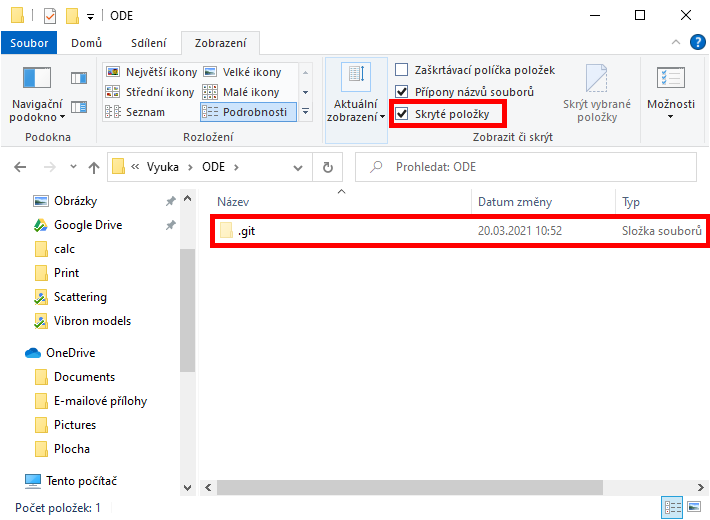
\includegraphics[width=0.7\linewidth]{FolderGit.png}\end{center}
    V této složce je uložena veškerá zapsaná historie vašeho projektu od jeho vytvoření.
    Pokud tuto složku smažete, přijdete tím o \uv{paměť} systému Git pro daný projekt, avšak aktuální soubory projektu zůstanou tak, jak jsou.
    Pokud naopak přesunete nebo překopírujete složku s projektem včetně podsložky \code{.git} kamkoliv jinam, klidně na jiný počítač, kopírujete zároveň celou historii projektu.
    Nedoporučuji jakkoliv měnit soubory v této skryté složce, protože tím můžete nevratně narušit integritu repozitáře a systém Git přestane být schopen repozitář používat.

\subsubsubsection{Stav repozitáře}
    Aktuální stav repozitáře kdykoliv zjistíte pomocí
    \begin{lstlisting}
        git status\end{lstlisting}
    Příkaz vypíše název aktuální větve a stav všech souborů v projektu.
    Pro čerstvě vytvořený repozitář se dozvíte něco takového:
    \begin{center}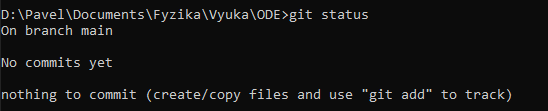
\includegraphics[width=0.6\linewidth]{GitStatusEmpty.png}\end{center}

\subsubsubsection{Vytvoření a první zapsání nového souboru}
    Ve složce s projektem otevřeme Visual Studio Code (napsáním \code{code} do příkazové řádky nebo stiskem pravého tlačítka myši nad otevřenou složkou a výběrem \uv{Open with Code}), vytvoříme nový soubor a uložíme ho jako \file{ode.py}.
    Příkaz \code{git status} ukáže
    \begin{center}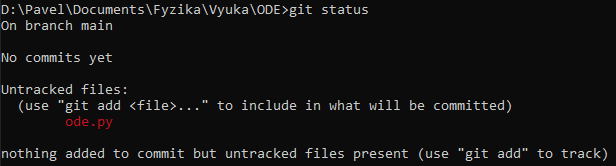
\includegraphics[width=0.7\linewidth]{GitStatusFirst.png}\end{center}
    Systém Git si je vědom toho, že si uživatel nemusí pamatovat všechny příkazy, a proto se snaží práci usnadnit a napovídá, které další akce lze v další fázi použít a jak.

    Příkazem \code{git add *} se nový soubor připraví k zapsání.
    Stav repozitáře se změní takto:
    \begin{center}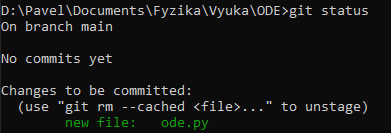
\includegraphics[width=0.45\linewidth]{GitStatusAdd.png}\end{center}

    Zapsání se provede příkazem \code{git commit}.
    Otevře se editor (nový soubor ve Visual Studiu Code), do kterého uvedeme stručný a výstižný popis změn:
    \begin{center}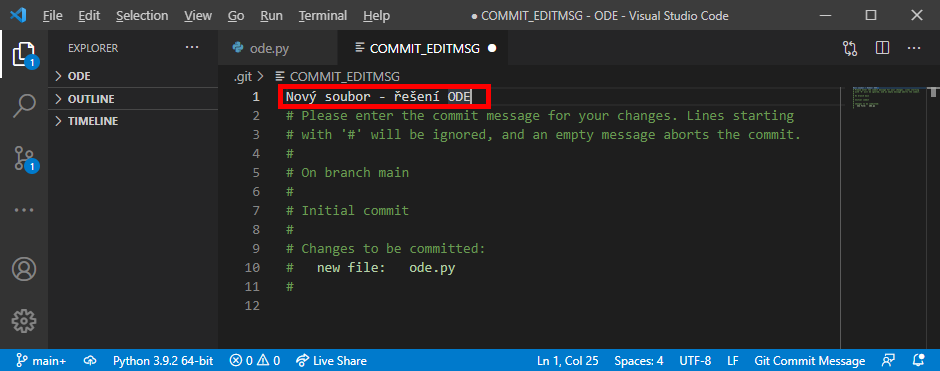
\includegraphics[width=0.9\linewidth]{VSCodeCommit.png}\end{center}
    Po uložení a zavření souboru se vytvoří první snímek historie našeho projektu.
    V příkazové řádce vidíme stručný souhrn, co se zapsalo.
    \begin{center}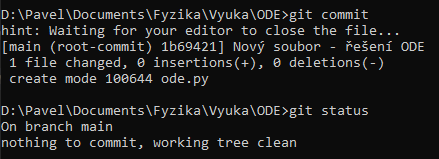
\includegraphics[width=0.5\linewidth]{GitStatusCommit.png}\end{center}

\subsubsubsection{Změny v souboru}
    Do souboru \file{ode.py} vepíšeme první část kódu, kterým bude řešení jedné diferenciální rovnice Eulerovou metodou 1. řádu.

    \begin{lstlisting}[style=TinyPython]
        def euler_1(model, y, t, dt):
            y1 = y + model(y, t) * dt
            t1 = t + dt
            return y1, t1
        
        def ode_solve(model, initial_condition, integrator=runge_kutta_4, dt=0.1, maxt=10):
            y = initial_condition                   # Initial conditions
            ys = [y]                                # List with results
            
            t = 0                                   # Actual time
            ts = [t]                                # List with times
            
            while t < maxt:
                y, t = integrator(model, y, t, dt)  # Step
                
                ys.append(y)                        # Store position
                ts.append(t)                        # Store time
                    
            return ys, ts
        
        def relaxation(y, t):
            return -y
        
        ys, ts = ode_solve(relaxation, 1)\end{lstlisting}
    Po spuštění kód vyřeší diferenciální rovnici relaxace~\eqref{eq:relaxace} a v proměnných \code{ys} a \code{ts} vrátí seznam $y$-ových hodnot a odpovídajících časových okamžiků $t$.

    Kód funguje a dává smysluplné výsledky ($y(t)$ klesá s rostoucím časem k nule), zapíšeme tedy změny do \uv{historie}.
    Stav repozitáře je
    \begin{center}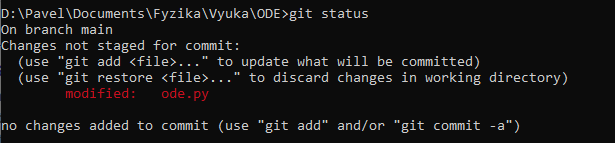
\includegraphics[width=0.7\linewidth]{GitStatusChange.png}\end{center}
    Soubor je ve stavu změněný (modified).
    Před zapsáním je nutné jeho stav změnit na k zapsání (staged) pomocí příkazu \code{git add *}.
    Lze také použít zkrácený příkaz
    \begin{lstlisting}
        git commit -a\end{lstlisting}
    který všechny změněné soubory převede do stavu k zapsání a rovnou zapsání provede.
    Změnu označním popisem \uv{Eulerova metoda 1. řádu}.
    \begin{center}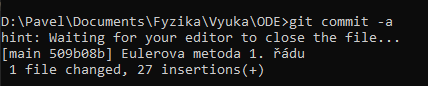
\includegraphics[width=0.5\linewidth]{GitStatusCommit2.png}\end{center}

    {\color{blue} Dobrá programátorská praxe je zapisovat vždy jen takový kód, který lze spustit, tj. který neobsahuje žádné syntaktické chyby.}

\subsubsubsection{Přidání dalšího souboru do projektu}
    V programu na řešení diferenciálních rovnic se bude hodit oddělit univerzální výpočetní funkce od funkcí specifických pro daný model.
    Vytvoříme tedy nový soubor \file{relaxation.py}, do kterého přesuneme kód
    \begin{lstlisting}[style=TinyPython]
        import ode

        def relaxation(y, t):
            return -y
        
        ys, ts = ode.ode_solve(relaxation, 1)\end{lstlisting}
    Nesmíme zapomenout náš \uv{modul} naimportovat pomocí příkazu \code{import ode}.
    Program lze spustit a funguje, je tedy dobrý čas tyto změny zapsat.
    Nejdříve se ale podíváme na stav repozitáře:    
    \begin{center}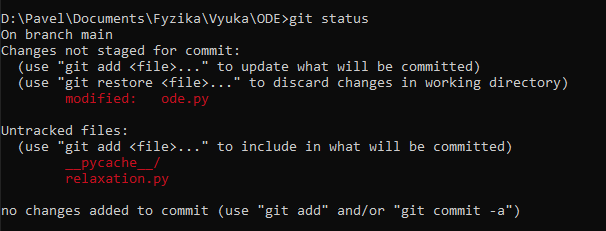
\includegraphics[width=0.7\linewidth]{GitStatusChange2.png}\end{center}
    Soubor \file{ode.py} se změnil, soubor \file{relaxation.py} byl vytvořen a zatím je ve stavu nesledován.
    Navíc se ještě vytvořila celá složka \file{__pycache__/}.\footnote{
        Pro urychlení provádění celého programu ukládá do tohoto adresáře interpret Pythonu speciálně předpřipravené používané moduly.
    }
    Jedná se o pomocnou složku, kterou verzovat nechceme.
    Toho se docílí buď tím, že ji ponecháme v nesledovaném stavu (untracked) a začneme sledovat jen nový soubor.
    Tento postup však znemožní používání hromadných příkazů \code{git add *} či \code{git commit -a}.
    Gitu lze speciálně naznačit, jaké soubory a jaké složky jsou jen pomocné, a má je tedy ignorovat.
    Za tím účelem se vytvoří speciální soubor pojmenovaný \file{.gitignore}, do kterého zapíšeme následující pravidlo
    \begin{lstlisting}
        __pycache__/\end{lstlisting}
    a uložíme.
    Stav repozitáře se změní následovně:
    \begin{center}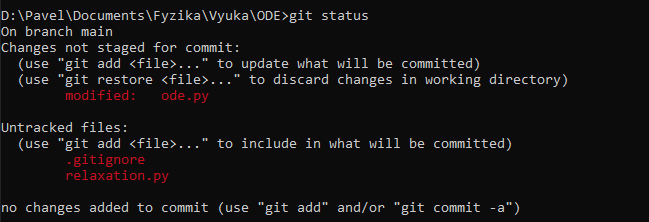
\includegraphics[width=0.7\linewidth]{GitStatusIgnore.png}\end{center}
    Pomocná složka už není uvedena mezi nesledovanými soubory a Git ji ignoruje.
    Můžeme již připravit k zapsání všechny nové a změněné soubory pomocí hromadného příkazu \code{git add *} a následně zapsat všechny změn pomocí \code{git commit},
    přičemž změnu pojmenuji \uv{Oddělení řešitele ODE a modelu}.

\subsubsubsection{Zobrazení historie revizí}
\label{sec:gitlog}
    Historie zobrazíme příkazem
    \begin{lstlisting}
        git log\end{lstlisting}
    \begin{center}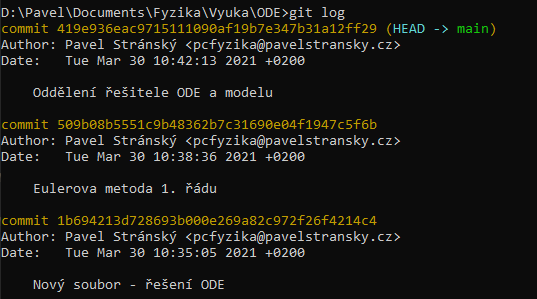
\includegraphics[width=0.7\linewidth]{GitLog.png}\end{center}
    Vypsaný seznam obsahuje všechny údaje o jednotlivých snímcích historie (zapsáních), tj. datum a čas, autora a jeho e-mail a hash kód podepisující zapsání.

    Příkaz log má velké možnosti, jak formátovat a filtrovat informace o zapsáních, přičemž všechny jsou uvedeny v \href{https://git-scm.com/docs/git-log}{referenční příručce}.
    Nejdůležitější jsou
    \begin{itemize}
        \item \code{git log -{}-oneline} naformátuje vše hezčím způsobem (každé zapsání na jednom řádku) a z hashe zobrazí jen prvních 7 znaků, což stačí k identifikaci jednotlivých zapsání,
        \item \code{git log -2} vypíše jen poslední dva záznamy,
        \item \code{git log -{}-stat} vypíše statistiky o jednotlivých verzích (počty změn a výpis změněných souborů),
        \item \code{git log -{}-graph} zobrazí výsledek \uv{graficky}, což se hodí v případě více větví (větve budou vysvětleny v sekci~\ref{sec:branches}),
        \item \code{git log -{}-follow ode.py} vypíše všechny historické změny v souboru \file{ode.py},
        \item \code{git log -{}-since "2 years 1 day 3 minutes ago"} 
        \item \code{git log -{}-until "2019-01-15"} vypíše všechny změny od, resp. do uvedeného časového údaje,
        \item \code{git log -{}-author="Pavel"} vypíše všechny změny, které zapsal uživatel Pavel,
        \item \code{git log -{}-grep="Euler"} vypíše všechny změny, které obsahují v popisu slovo \uv{Euler}.
    \end{itemize}
    Uvedené filtry lze samozřejmě libovolně kombinovat.

\subsubsection{.gitignore}
\label{sec:gitignore}
    Překladače programovacích jazyků často vytvářejí v adresáři projektu dočasné pomocné soubory, které nechcete, aby se staly součástí repozitáře (tyto soubory nenesou žádnou relevantní informaci, navíc mohou na různých počítačích vypadat jinak podle toho, jaký překladač či jaké vývojové prostředí zrovna použijete).
    Abyste mohli používat příkazy pro hromadné sledování či zapisování souborů \code{git add *} či \code{git commit -a}, musíte GITu naznačit, jaké soubory má ignorovat.
    K tomu slouží soubor \code{.gitignore}.
    
    Každé pravidlo v souboru \code{.gitignore} zabírá jeden řádek.
    Řádek, který začíná znakem \#, je ignorován a může sloužit například jako komentář.
    Příklady jednotlivých řádků:
    \begin{itemize}
    \item \code{tajne.txt}
        
        Ignoruje soubor s názvem \code{tajne.txt} (může obsahovat třeba přihlašovací údaje k nějaké službě a ty rozhodně nechceme sdílet ani archivovat; nezapomeňte, že co je jednou zapsané v repozitáři, z něj až na výjimky nelze odstranit).

    \item \code{*.log}
    
        Ignoruje všechny soubory s příponou \code{log},

    \item \code{!important.log}

        avšak neignoruje soubor \code{important.log}.

    \item \code{*.[oa]}

        Ignoruje všechny soubory s příponou \code{o} nebo \code{a}.

    \item \code{temp/}

        Ignoruje všechny soubory v podsložce \code{temp}.

    \item \code{doc/**/*.pdf}
    
        Ignoruje všechny soubory s příponou \code{pdf} v podsložce \code{doc} a ve všech jejích podsložkách.
        Neignoruje však soubory s příponou \code{pdf} v kořenové složce projektu.
    \end{itemize}
    Další příklady použití souboru \code{.gitignore} jsou například~\href{https://www.atlassian.com/git/tutorials/saving-changes/gitignore}{na této stránce}.

    Pokud na GitHubu zakládáte nový projekt, můžete upřesnit, jaký programovací jazyk budete používat a GitHub automaticky vytvoří optimální soubor \code{.gitignore}.

    \begin{voluntary}
        Podívejte se do souboru \ghfile{}{.gitignore} v repozitáři k těmto zápiskům.
        Zatímco Python si téměř žádné pomocné soubory nevytváří, {\LaTeX} jich generuje požehnaně.
        Proto je seznam ignorovaných souborů celkem dlouhý. 
    \end{voluntary}

\subsubsection{Větve}
\label{sec:branches}
    Verzovací systém Git umožňuje pracovat paralelně na několika různých verzích kódu a mezi nimi dokáže efektivně přepínat.
    Větvení se hodí v případě, že chceme vyzkoušet více různých přístupů k řešení úlohy.
    Pro každý nápad vytvoříme vlastní větev úprav, což dovolí řešení porovnávat a nakonec vybrat to, které vyhovuje nejvíce.
    Každou větev můžeme dále větvit.
    Změny v perspektivních větvích lze následně začleňovat do hlavní větve, neperspektivní větve lze nechat být nebo odstranit.
    
    Častá programátorská praxe je taková, že v hlavní větvi\footnote{Hlavní větev se donedávna pojmenovávala \code{master}, dnes se spíše prosazuje pojmenování \code{main}.} se nachází vždy jen odladěná a otestovaná verze programu.
    Pro každou změnu v projektu se vytvoří nová větev.
    Na té se může pracovat hodinu, ale třeba několik měsíců.
    V této \uv{vývojové} větvi se změny provedou, odladí, pošlou testerům, a teprve po důkladném otestování se začlení do hlavní větve.
    Mezitím je stále k dispozici funkční program hlavní větve, který lze bez obav používat k ostrému provozu.

\subsubsubsection{Vytvoření nové větve}
    Budeme pokračovat ve vývoji programu pro řešení obyčejných diferenciálních rovnic.
    Předpokládejme, že řešení pro jednu rovnici máme hotové a chceme ho rozšířit tak, aby fungovalo i na soustavu libovolného počtu diferenciálních rovnic 1. řádu, kterým se věnuje sekce~\ref{sec:ODRn}.
    K tomu vytvoříme novou větev \code{odesystem}
    \begin{lstlisting}
        git branch odesystem\end{lstlisting}
    a přepneme se na ni příkazem\footnote{
        Vytvoření nové větve a přepnutí se do ní lze jedním příkazem \code{git switch -c odesystem}.
    }
    \begin{lstlisting}
        git switch odesystem\end{lstlisting}
        Zpět na hlavní větev se lze vrátit příkazem \code{git switch main}.\footnote{
            Git umožňuje přepínání mezi větvemi také pomocí příkazu \code{git checkout}.
        }

\subsubsubsection{Výpis větví}
    Seznam všech větví se vypíše příkazem
    \begin{lstlisting}
        git branch\end{lstlisting}
    \begin{center}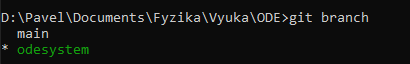
\includegraphics[width=0.45\linewidth]{GitBranch.png}\end{center}
    Aktivní větev je vyznačena hvězdičkou i barevně.

    Další užitečná upřesnění výpisu větví jsou
    \begin{itemize}
        \item \code{git branch -{}-merged} vypíše jen větve spojené s aktuální větví,
        \item \code{git branch -{}-no-merged} vypíše jen větve nespojené s aktuální větví.
    \end{itemize}

\subsubsubsection{Změny a sloučení větví}
    Poté, co provedeme a odladíme změny související s rozšířením programu na výpočet soustavy diferenciálních rovnic ve větvi \code{odesystem}, můžeme tyto změny začlenit do hlavní větve \code{main}.
    K tomu slouží příkaz
    \begin{lstlisting}
        git merge odesystem\end{lstlisting}
    spuštěný v hlavní větvi.
    Pokud během slučování nedojde k žádným konfliktům, vše proběhne hladce.
    Může se však stát, že byly provedeny změny na stejném místě jednoho souboru v obou větvích (konflikt).
    V tom případě Git označí konflikty v souborech a jejich stav změní na modifikovaný.
    Pak je potřeba tyto soubory projít, vybrat z konfliktních verzí jednu, případně kód upravit tak, aby odrážel obě konfliktní změny, a zapsat příkazem \code{git commit -a}.
    Tím je slučování dokončeno.    
    
\subsubsubsection{Odstranění větve}
    Větev odstraníme prostým
    \begin{lstlisting}
        git branch -d odesystem\end{lstlisting}
    Odstraňovat větve má smysl jen v případě, kdy jsme přesvědčeni, že změny v ní provedené byla slepá cesta, nebo pokud provedené změny byly začleněny do jiné větve.

\subsubsection{Návrat k dřívějším verzím}
    {\color{red} Pozor, při neopatrném použití těchto příkazů hrozí ztráta dat!}
    Pokud si budete následující příkazy zkoušet, doporučuji vám zazálohovat si celou složku s projektem včetně repozitáře (složky \file{.git}).

    \begin{itemize}
        \item \code{git commit -{}-amend} umožňuje změnit popis posledního zapsání.
        \item \code{git restore soubor} vrátí změny uvedeného souboru na posledně zapsanou verzi (lze použít i hromadné \code{git restore *}\footnote{\code{git restore *} se chová podobně jako \code{git reset -{}-hard}.}).
        \item \code{git reset HEAD\~{}1} zruší poslední\footnote{Číslo udává, o kolik revizí se vracíme zpět.} zapsání, avšak soubory ve složce projektu ponechá tak, jak jsou.\footnote{HEAD vlastně značí ukazatel na poslední zapsání.}
        \item \code{git reset -{}-hard HEAD\~{}1} zruší poslední zapsání a soubory projektu uvede do stavu, v jakém byly na začátku této poslední revize. 
        Všechny provedené změny jsou nenávratně ztraceny.
        Pokud byl nějaký soubor v poslední revizi vytvořen, je smazán.
        Toto je nejnebezpečnější příkaz, proto používejte jen v opravdu odůvodněných případech.
        \item \code{git reset 946cb25} se vrátí na zapsání, jehož hash začíná uvedeným číslem.
        \item \code{git reset ORIG_HEAD} se vrátí na tu zapsanou verzi, na které jsme byli bezprostředně před použitím posledního příkazu \code{git reset}.
        \item \code{git checkout -b oldrev 946cb25} vytvoří novou větev nazvanou \uv{oldrev}, ve které budou soubory ve stavu, kdy bylo provedeno zapsání s uvedeným hashem (hash zjistíme například pomocí \code{git log -{}-oneline} popsaného v sekci~\ref{sec:gitlog}).
        \item \code{git checkout 946cb25} vrátí se do tohoto zapsání, ale ponechá historii tak, jak je.\footnote{Tzv. detached HEAD state.}.
            K návratu zpět stačí použít příkaz pro přepnutí do hlavní větve \code{git switch main}.
    \end{itemize}

\subsubsection{Vzdálené repozitáře}\label{sec:GITRemote}
    Verzovací systém GIT umí kromě sledování a uchovávání historie změn souborů vašeho projektu i koordinovat změny, které provádí na projektu více řešitelů (pracovní tým). 
    K tomu slouží vzdálené repozitáře.
    Mezi nejrozšířenější systémy patří
    \begin{itemize}
    \item \href{https://github.com}{GitHub}: 
        Na něm si každý může zdarma zřídit vlastní repozitáře a používat je například k~synchronizaci svého projektu mezi různými počítači, pro sdílení vlastních výtvorů s komunitou nebo právě pro spolupráci ve vlastním týmu. 
        Vlastníkem firmy vyvíjející tento systém je Microsoft, díky čemuž je základní práce s ním integrována do vývojového prostředí Visual Studio Code.
    \item \href{https://gitlab.mff.cuni.cz}{GitLab}: 
        Open source řešení, základní verze rovněž zdarma, k pokročilé verzi má MFF UK licenci.
    \end{itemize}
    Oba systémy disponují webovým rozhraním, ze kterého lze projekty jednoduše spravovat, a~rovněž desktopovými aplikacemi, které umožňují pracovat s lokálními repozitáři pomocí jednoduchého rozhraní.
    Pro GitHub existuje například \href{https://desktop.github.com}{GitHub Desktop}.
    Projekty mohou být buď soukromé (přístup k nim máte pouze vy či ti, kterým pošlete pozvánku), nebo veřejné (přístup má zcela kdokoliv).

    Tyto zápisky a vzorové ukázky kódů jsou veřejně na GitHubu a můžete k nim dostat na adrese \url{https://github.com/PavelStransky/PCInPhysics}.
    K dispozici je samozřejmě celý repozitář s historií se všemi commity a se všemi vývojovými větvemi.
    Repozitář můžete stáhnout buď z uvedené webové stránky (zelené tlačítko \code{Clone or download}), nebo pomocí programu git.

    \begin{itemize}
    \item \code{git clone https://github.com/PavelStransky/PCInPhysics}
    
        V aktuální složce vytvoří podsložku \code{PCInPhysics} a do ní stáhne celý repozitář.
        V případě těchto zápisků se jedná o tento soubor v {\LaTeX}u,
        výsledné PDF, EPS či PNG verze všech obrázků a všechny zdrojové kódy.

    \item \code{git remote -v}
    
        V adresáři s lokálním repozitářem ukáže, na jaký vzdálený repozitář je navázaný.
        Stejně jako základní větev se standardně jmenuje \code{main}, vzdálený repozitář se standardně jmenuje \code{origin}.
        Vy můžete mít na jeden projekt navázáno více vzdálených repozitářů, každý pak samozřejmě musíte pojmenovat jinak.

    \item \code{git remote add origin https://github.com/Uzivatel/VzdalenyRepozitar}
    
        Přidá do vašeho projektu odkaz na vzdálený repozitář umístěný na GitHubu.

    \item \code{git remote show origin}
    
        Zobrazí informace o vzdáleném repozitáři.

    \item \code{git pull}
    
        Do adresáře s lokálním repozitářem stáhne aktuální verzi aktuální větve.
        Pokud máte lokálně rozpracované změny, stažení se nepovede.
        Pokud máte uložené změny (commit), git se automaticky pokusí vaše změny sloučit se změnami v globálním repozitáři (merge).
        
    \item \code{git push origin master}
    
        Do vzdáleného repozitáře \code{origin} zapíše vaši větev \code{master}.
        Vzdálený repozitář může být nastaven tak, že vaše změny musí ještě někdo schválit.

    \item \code{git push}

        Zkrácený zápis, pokud jste dříve nastavili pomocí příkazu \code{git push --set-upstream origin master} název lokální větve a příslušného vzdáleného repozitáře.

    \end{itemize}

    Další informace najdete například v \href{https://git-scm.com/book/cs/v2/Z%C3%A1klady-pr%C3%A1ce-se-syst%C3%A9mem-Git-Pr%C3%A1ce-se-vzd%C3%A1len%C3%BDmi-repozit%C3%A1%C5%99i}{dokumentaci}.

    \begin{voluntary}
        Stáhněte si do svých počítačů (naklonujte si) z GitHubu repozitář s poznámkami k tomuto cvičení.
        V budoucnu si pomocí příkazu \code{git pull} stahujte aktuální verze.
        Můžete si vytvořit pracovní větev poznámek a v ní si s kódy hrát.
        V hlavní větvi \code{master} se vám uchová originální verze ze~vzdáleného repozitáře.
    \end{voluntary}

    \begin{voluntary}
        Vytvořte si účet na GitHubu, vytvořte prázdný projekt a navažte si ho s dříve na cvičení vytvořeným lokálním repozitářem pomocí příkazů \code{git remote add} (plný příkaz výše).
        Následně si do vzdáleného repozitáře nahrajte lokální repozitář pomocí příkazu \code{git push}. 
    \end{voluntary}

\subsubsection{Tahák}
    Pro snadnou orientaci v použití Gitu bez nutnosti pamatovat si všechny příkazy je dostupný \href{https://training.github.com/downloads/github-git-cheat-sheet.pdf}{Git Cheat Sheet} nebo \href{https://ndpsoftware.com/git-cheatsheet.html}{tento interaktivní web}.

\subsection{Programovací jazyk Python}
    Python je v dnešní době velmi populární programovací jazyk, který pronikl do spousty rozmanitých odvětví, a to zejména díky bohatosti a pokročilosti knihoven, které jsou vyvíjeny komunitou a jsou díky tomu aktuální a odladěné (či průběžně odlaďované).
    Python existuje na mnoha platformách od osobních počítačů po mikrokontroléry a dá se v něm naprogramovat téměř cokoliv: pokročilé vědecké výpočty používající nejnovější numerické algoritmy, dobře vypadající grafy, statistická analýza, analýza velkých dat a strojové učení, ale také webové služby, okénkové programy či editace obrázků a videí.
    Je běžné, že i komerční programy obsahují Python coby skriptovací jazyk, čímž umožňují uživateli používat své vlastní kódy \uv{uvnitř} komerčního produktu a integrovat různé programy mezi sebou.\footnote{
        Jako příklad poslouží nejnovější verze programu \href{https://www.wolfram.com/language/12/external-system-integration/evaluate-python-in-a-notebook.html}{Mathematica}, \href{https://www.originlab.com/doc/python/Run-Python-in-Origin}{Origin} či \href{https://developer.sas.com/guides/python.html}{SAS}.
    }
    
    Python lze charakterizovat jako jazyk:
    \begin{itemize}
        \item 
            \emph{Interpetovaný}, což znamená, že provádění programů probíhá přímo ze zdrojového kódu.\footnote{
                Mezi další známé interpetované jazyky patří napříkad JavaScript nebo PHP.
            }
            Ke spouštění kódů je tedy potřeba mít nainstalovaný interpret, což jsme učinili v sekci~\ref{sec:InstalacePython}.
            Pokud kód obsahuje syntaktickou chybu, je odhalena až ve chvíli, kdy se na ni interpret při provádění kódu narazí.
            U interpretovaných jazyků se neztrácí čas překladem do strojového kódu a je pro ně přirozené dynamické typování proměnných.
            Tím, že interpet čte text kódu příkaz po příkazu, je provádění programů pomalejší, ale vzhledem k tomu, že velká část časově náročných funkcí a knihoven bývá napsána v rychlejších programovacích jazycích, není to zásadní nevýhoda.
            Kvůli skutečnosti, že Python se obvykle používá jako mezičlánek spojující efektivně napsané funkce různých knihoven, setkáte se také s označením jazyk \emph{skriptovací}.
            
            Opakem intepretovaných jazyků jsou jazyky kompilované, přičemž kompilace se provádí buď přímo do strojového kódu daného procesoru\footnote{Například C/C++, Pascal nebo Fortran.} nebo do mezikódu. 
            Mezikód ke spuštění vyžaduje dodatečnou kompilaci, která však může být vysoce optimalizovaná přímo pro danou hardwarovou konfiguraci použitého počítače.\footnote{
                Zde se jedná napřílad o jazyky Java, C\# a celý .NET framework nebo Julia.
                }\footnote{
                    Pro Python existuje knihovna \file{\href{https://numba.pydata.org/}{Numba}}, která také umožňuje překlad vybraných částí programu do strojového kódu pomocí \href{https://llvm.org/}{LLVM} překladače, a tím provádění programu výrazně zrychlit.
                }

        \item 
            \emph{Dynamicky typovaný}, což znamená, že proměnná nemusí mít předem daný typ a typ proměnné se může za běhu programu dokonce měnit.
        
        \item 
            \emph{S automatickou správou paměti}, takže programátor se nemusí starat o alokování a uvolňování paměti. 
            Python při inicializaci proměnné paměť alokuje automaticky a ve chvíli, kdy proměnnou přestaneme používat, paměť uvolní.\footnote{Algoritmus se nazývá \emph{Garbage collection}.} 

        \item
            V Pythonu lze pythonovským způsobem používat tři základní programovací paradigmata: \emph{procedurální, objektové a funkcionální}.
    \end{itemize}
         
    Python klade důraz na jednoduchost, stručnost a čitelnost kódu.
    Filosofie programovacího jazyka je shrnuta v \href{https://www.python.org/dev/peps/pep-0020/}{Zenu Pythonu},\footnote{
        Zen se také vypíše, pokud do svého kódu zadáte \code{import this}.
    } se kterým vám doporučuji se seznámit.

\subsubsection{Vytvoření a spuštění kódu}
    Ve Visual Studio Code vytvoříme nový soubor a uložíme si ho s příponou \code{*.py}. 
    Podle této přípony VS Code pozná, že se jedná o pythonovský kód a použije k práci s ním správný doplněk.
       
    Hotový kód lze spustit ve VS Code jedním z následujících tří způsobů.
    \begin{enumerate}
        \item 
            \emph{Kliknutím na šipku na nástrojové liště}:
            Tímto způsobem se spustí celý soubor kódu.
            \begin{center}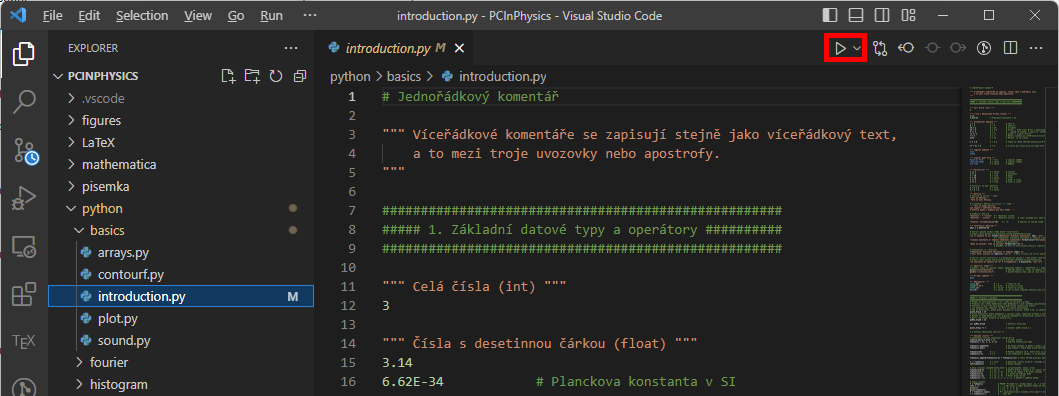
\includegraphics[width=\linewidth]{PythonRun.png}\end{center}
        \item
            \emph{Stiskem \code{F5}}: Kód se spustí v režimu ladění (debugger).
            Zastaví se na každém kontrolním bodě (breakpoint, který se vloží na vybranou řádku kódu klávesou \code{F9}) nebo na každé chybě.
            Pro pokračování provádění kódu stačí stisknout buď znovu \code{F5}, nebo \code{F10} či \code{F11} pro jeden krok.

        \item
            \emph{Označením části kódu a stiskem \code{Shift+Enter}}: V okně \code{TERMINAL} spustí \abbreviation{REPL} Pythonu a v něm označenou část kódu.
            \abbreviation{REPL} se po provedení kódu nezavře, takže v něm lze psát dodatečné příkazy.
            Pro ukončení \abbreviation{REPL} do něj stačí napsat \code{exit()} nebo v něm stisknout \code{Ctrl+Z} a potvrdit nebo ukončit okno terminálu kliknutím na ikonku popelnice.
    \end{enumerate}

\subsubsection{Základy syntaxe Pythonu}
    Soubor se vzorovými příklady najdete v repozitáři ke cvičení: \ghfile{python/basics/}{introduction.py}.\footnote{
        Vzorový soubor je inspirován příkladem \href{https://learnxinyminutes.com/docs/cs-cz/python/}{Nauč se Python v Y minutách}.
    }
    Doporučuji vám si ho stáhnout nebo jeho obsah překopírovat a důsledně si ho řádek po řádku projít a spouštět nejlépe pomocí označení a stiskem \code{Ctrl+Enter}, jak bylo popsáno v předchozí sekci.
    Některé části kódu odkazují na proměnné zavedené v dřívější části souboru, proto kód procházejte postupně od začátku do konce.

    Z vzorového kódu bych vypíchl následující body:
    \begin{enumerate}
        \item 
            \emph{Základní datové typy a operátory:}
            Python obsahuje jen dva základní číselné typy: \code{int} a \code{float}.
            Jejich použití je podobné jako v jiných programovacích jazycích.

        \item
            \emph{Formátování řetězců:}
            Python umožňuje několik různých způsobů, jak formátovat řetězce (vkládat do nich čísla či jiné proměnné).
            Doporučuji se seznámit s velmi čitelným způsobem pomocí \code{f}-řetězce.            
            Více informací k formátování řetězců naleznete v tomto výborném \href{https://pyformat.info}{návodu}.
    
        \item
            \emph{Proměnné a kolekce:} 
            Důležité standardní kolekce jsou \emph{seznam} (list) [...] a \emph{slovník} (dicctionary) \{...\}.
            Dále existuje typ \emph{n-tice} (tuple) (...) a \emph{množina} (set) \{...\}.
            O jaký typ kolekce se jedná poznáte podle typu závorek, kterými je uzavřena.
            Python nabízí bohaté možnosti indexování prvků kolekcí.

            Python nemá typ \uv{řada} (jedno či vícerozměrný soubor hodnot stejných typů).
            Ten je implementován až v rozšiřujících knihovnách, například v knihovně \file{numpy}, které je věnována sekce~\ref{sec:numpy}.
            
        \item
            \emph{Podmínky a cykly}:
            Příkaz uvozující blok kódu vždy končí znakem \uv{:}.
            Každý blok je definován svým odsazením, které musí být na každém řádku stejné
            (tj. musí obsahovat stejný počet odsazujících znaků, mezi které patří buď mezera nebo tabulátor).
            Konvence je používat k odsazení \href{https://www.python.org/dev/peps/pep-0008/#indentation}{4 mezery}.

            Cykly jsou možné pouze přes iterovatelné objekty.
            Pro cyklus přes přirozená čísla (indexy) musíme vytvořit odpovídající iterovatelný objekt příkazem \code{range}.
            V drtivé většině případů se lze při programování v Pythonu indexům zcela vyhnout.

        \item 
            \emph{Funkce}: Python umožnuje velkou variabilitu co se týče argumentů funkce a návratových hodnot díky své funkci automatického sbalení a rozbalení kolekcí.
            Funkce se navíc chová jako objekt, lze ji tedy přiřadit jakékoliv proměnné.
            To je jeden z prvků funkcionálního programování.

            Funkcionální programování také obsahuje koncept anonymní funkce, což je jednoduchá funkce definovaná na jednom řádku, která nemá vlastní jméno.
            V Pythonu se vytváří pomocí klíčového slova \code{lambda}.

        \item 
            \emph{Moduly}: Při programování je důležité vhodně strukturovat kód.
            Python obsahuje jednoduchý koncept modulů, přičemž každý soubor s příponou \code{*.py} lze použít jako modul.
            Modul je vlastně speciální typ objektu.

            Dobře se seznamte se způsoby, jak modul načíst a používat, jelikož většina funkcí Pythonu se nachází právě v modulech.
            Jedná se například o matematické funkce v modulu \file{math} nebo rozšiřující knihovny \file{numpy}, \file{scipy} a \file{matplotlib}.

        \item 
            \emph{Třídy}: Python umožňuje objektově orientované programování.
            Práce s třídami se však v mnohém liší od striktně objektově orientovaných programovacích jazyků, jakými jsou například C++, C\# nebo Java.
            Důležitý rozdíl je například v přístupnosti atributů (všechny atributy v Pythonu jsou veřejné).
            Rovněž dědičnost a dědění metod se chová odlišně.
            Dále je nutné pamatovat na to, že každá metoda třídy musí mít v deklaraci jako první argument odkaz na instanci, se kterou je volána (konvenčně se označuje \code{self}).
            Ve vzorovém kódu je k objektovému programování opravdu jen to nejnutnější minimum.
            Pokud chcete v Pythonu využívat objekty seriózně, doporučuji pročíst si odpovídající \href{https://docs.python.org/3/tutorial/classes.html}{kapitolu v manuálu}.
    \end{enumerate}

    Uvedený kód s příklady obsahuje jen ty struktury jazyka Python, které budeme používat.
    V budoucích cvičeních se ještě seznámíte se \emph{správou kontextu} (klíčové slovo \code{with}).
    Python umožňuje navíc 
    \begin{itemize}
        \item ošetření chyb pomocí \emph{výjimek} (klíčová slova \code{raise}, \code{try}, \code{except}, \code{finally}),
        \item tvorbu \emph{generátorů} (klíčové slovo \code{yield}),
        \item \emph{asynchronní programování}, korutiny a úkoly (klíčová slova \code{await}, \code{async})
        \item či tvorbu a použití \emph{dekorátorů}.
    \end{itemize}
    Pro plné ovládnutí jazyka vám doporučuji se v budoucnu s těmito koncepty seznámit, a to buď na dedikovaných přednáškách, z tutoriálů a návodů na webu, nebo studiem cizích kódů.

    Na oficiálních stránkách Pythonu najdete \href{https://docs.python.org/3/tutorial/}{tutoriál k nejnovější verzi programovacího jazyka}.

\subsubsection{Pojmenování proměnných a formátování}
    Formátování kódu Pythonu je celkem volné.
    Povinné je dodržet jen správné odsazení bloků.
    Pro snazší čitelnost kódu byla nicméně vytvořena řada doporučení, která najdete souhrnně na stránce \href{https://www.python.org/dev/peps/pep-0008}{PEP 8}.\footnote{\abbreviation{PEP} = {\bf P}ython {\bf E}nhancement {\bf P}roposal}
    Python obsahuje dokonce knihovnu \file{\href{https://pypi.org/project/autopep8/}{autopep8}}, která váš zdrojový soubor podle těchto pravidel naformátuje.
    Automatické formátování podle PEP 8 lze nastavit i ve \href{https://code.visualstudio.com/docs/python/editing#_formatting}{Visual Studiu Code}.
        
    Pro pojmenování proměnných existuje jediné závazné pravidlo, které zní, že indentifikátor se nesmí shodovat s žádným z \href{https://docs.python.org/3/reference/lexical_analysis.html#keywords}{35 klíčových slov} jazyka.
    Kromě toho jsou ve výše uvedeném dokumentu další nezávazná pravidla k pojmenování proměnných:\footnote{
        Čitelnosti různých stylů pojmenování proměnných se věnují i seriózní vědecké články, například
        \url{http://www.cs.kent.edu/~jmaletic/papers/ICPC2010-CamelCaseUnderScoreClouds.pdf}.
    }
    \begin{itemize}
        \item
            \emph{Proměnné a funkce} se doporučuje pojmenovávat malými písmeny a jednotlivá slova spojovat podtržítky, tzv. underscore style (například \code{pocet_bodu}).
        \item
            \emph{Konstanty} se doporučuje pojmenovávat velkými písmeny a jednotlivá slova spojovat podtržítky (například \code{PLANCKOVA_KONSTANTA}).
        \item
            \emph{Třídy} se doporučuje pojmenovávat tak, že jednotlivá slova názvu začínají velkým písmenem a mezi nimi není žádný znak, tzv. Pascal style (například \code{PostovniAdresa}).
        \item
            \emph{Moduly} se doporučuje pojmenovávat krátkými výstižnými názvy složenými jen z malých písmen.
        \item
            Kvůli čitelnosti je dobré se vyhnout jednopísmenným označením \code{l}, \code{I} a \code{O}, jelikož takto označené proměnné mohou být snadno zaměněny s čísly \code{1} a \code{0}.

    \end{itemize}
    Pokud vám vyhovuje jiný styl pojmenovávání, lze ho použít.
    Je však dobré být v pojmenovávání konzistentní napříč celým projektem.

    Častá otázka je, zda proměnné označovat \emph{česky či anglicky}.
    Jelikož nikdy nevíte, kdo v dnešním propojeném světě bude chtít váš kód použít a třeba i upravit pro své potřeby, doporučuji používat anglická pojmenování.
    
    Snadná čitelnost kódu je podpořena i správným psaním \emph{komentářů}.
    Předně se dnes doporučuje vycházet z předpokladu, že dobře napsaný kód je čitelný i bez komentářů.
    Čitelnost totiž zaručují zejména vhodně a výstižně označené proměnné a správně navržená struktura kódu.
    Komentovat je dobré jen ty části kódu, kde se používá nějaký ne všeobecně známý trik nebo postup.
    Nadbytek komentářů je velmi těžké udržovat při úpravách a může vést i k tomu, že po několika změnách kódu nebudou komentáře v souladu s tím, co kód vykonává.
    
    Naopak doporučené je nešetřit popisem, co dělají jednotlivé funkce, jaké jsou jejich argumenty a co vracejí na výstupu.
    K tomu slouží komentář typu \emph{docstring}, který je vysvětlený v souboru \ghfile{python/basics/}{introduction.py} v sekci o funkcích.\footnote{
        Stejně jako v mluvených jazycích se zlepšujete čtením literatury, v programovacích jazycích pomáhá čtení cizích kódů.
        Pro příklad použití komentářů se koukněte třeba na zdrojový soubor funkce \code{\href{https://github.com/scipy/scipy/blob/master/scipy/optimize/optimize.py}{optimize}} z knihovny \file{scipy}.
    }
    Použití \emph{docstringu} usnadní i tvorbu a správu doprovodné dokumentace k celému projektu.
    Existují dokonce nástroje, které vám z těchto komentářů vytvoří strukturované webové stránky, například nástroj~\href{https://www.sphinx-doc.org}{Sphinx}.

\subsubsection{Řady, vektory, matice}
\label{sec:numpy}
    Jak bylo zmíněno v předchozí sekci, definice jazyka Python neobsahuje typ \emph{řada}, tj. jedno či vícerozměrně pole hodnot stejného typu.
    Tento typ a operace s ním jsou implementovány v knihovně \file{numpy}.
    Ta není v holé instalaci Pythonu obsažena, je nutné ji doinstalovat podle návodu v sekci~\ref{sec:pip}.
    Základy práce s řadami jsou vysvětleny v souboru \ghfile{python/basics/}{arrays.py} v repozitáři.

\subsubsection{Grafy}
    K vykreslení grafů se nejčastěji používá knihovna \file{\href{https://matplotlib.org}{Matplotlib}}.
    V základní instalaci Pythonu není obsažena, je nutné ji doinstalovat podle návodu v sekci~\ref{sec:pip}.
    Jednoduchý příklad vykreslení grafů je v souboru \ghfile{python/basics/}{plot.py} v repozitáři.

\subsubsection{Pseudonáhodná čísla}\label{sec:PseudonahodnaCisla}
    V Pythonu lze pseudonáhodná čísla generovat pomocí několika knihoven.
    \begin{itemize}
        \item 
            Pro základní použití je k dispozici knihovna \file{\href{https://docs.python.org/3/library/random.html}{random}}.
            Z ní nejdůležitější funkce jsou tyto:
            \begin{itemize}
                \item \code{random()}: Pseudonáhodné číslo $x$ rovnoměrně vybrané z intervalu $x\in\langle 0;1)$.
                \item \code{uniform(a, b)}: pseudonáhodné číslo $x$ rovnoměrně vybrané z intervalu $x\in\langle a;b\rangle$.
                \item \code{gauss(mu, sigma)}: pseudonáhodné číslo z Gaussovského rozdělení se střední hodnotou \code{mu} a směrodatnou odchylkou \code{sigma}. 
                \item \code{randint(a, b)}: pseudonáhodné \emph{celé} číslo $d$ z intervalu $a\leq d<b$.
                \item \code{seed(s)}: nastaví počáteční násadu generátoru podle parametru \code{s} (pro jednu konkrétní násadu bude generátor dávat stejnou sekvenci čísel). 
                Parametr může být jakéhokoliv typu, tedy číslo, řetězec atd. 
                Pokud se parametr neuvede, použije se jako násada aktuální systémový čas, a tudíž bude sekvence pseudonáhodných čísel při každém spuštění programu jiná.
                \item \code{choice(m)}: vybere pseudonáhodně element ze seznamu \code{m}.
                \item \code{shuffle(m)}: promíchá elementy v seznamu \code{m}.
            \end{itemize}

        \item
            Ke generování řad či vícerozměrných objektů, jejichž elementy jsou náhodná čísla, lze použít i knihovnu \file{numpy}, viz sekce~\ref{sec:numpy} a soubor s příklady~\ghfile{python/basics/}{numpy.py}.

        \item 
            Pro pokročilejší použití je knihovna \file{\href{https://numpy.org/doc/stable/reference/random/index.html}{numpy.random}}.
            Ta umožňuje zvolit vlastní generátor pseudonáhodných čísel, generovat čísla z celé řady \href{https://numpy.org/doc/stable/reference/random/generator.html}{statistických rozdělení} a generovat naráz celé vektory či matice.
            \begin{itemize}
                \item \code{generator = default_rng()}: Inicializuje standardní generátor pseudonáhodných čísel.
                \item \code{generator = Generator(PCG64())}: Inicializuje specifický generátor pseudonáhodných čísel (v~tomto případě PCG-64, což je O'Neillův \href{https://en.wikipedia.org/wiki/Permuted_congruential_generator}{permutační kongruenční generátor}).
                \item \code{generator.random(size=10)}: vektor délky 10 s elementy z rovnoměrného rozdělení na~intervalu $\langle 0;1)$.
                \item \code{generator.normal(size=10)}: vektor délky 10 s elementy z normálního Gaussova rozdělení se střední hodnotou $0$ a směrodatnou odchylkou $1$.
                \item \code{generator.normal(loc=1, scale=2, size=(10,10))}: matice rozměru $10\times10$ s elementy z normálního Gaussova rozdělení se střední hodnotou $1$ a směrodatnou odchylkou~$2$.
            \end{itemize}            
    \end{itemize}

\subsubsection{Práce se zvukem}
\label{sec:Zvuk}
    V Pythonu existuje velké množství knihoven, které umějí pracovat se zvukem.
    Pro naše účely postačí jednoduchá knihovna \href{https://python-sounddevice.readthedocs.io}{sounddevice}.\footnote{
        Další knihovny pro přehrávání a nahrávání zvuku jsou uvedeny na \url{https://realpython.com/playing-and-recording-sound-python}.
    }
    Pokud ji nemáte nainstalovanou, doinstalujete ji příkazem
    \begin{align*}
        &\texttt{python -m pip install sounddevice}
        &&\text{Windows}\\
        &\texttt{pip install sounddevice}
        &&\text{Linux, Mac}
    \end{align*}
    Z této knihovny využijeme následující funkce:
    \begin{itemize}
        \item \code{play(data, fs)} 
            přehraje časovou řadu uloženou v poli \code{data} při vzorkovací frekvenci \code{fs}.
            Jsou-li elementy přehrávané řady typu \code{float}, jejich hodnoty musejí ležet v rozmezí $h_{j}\in\langle-1,1\rangle$, jinak bude zvuk přebuzený a zkreslený.
            Vzorkovací frekvence zvukových souborů bývají nejčastěji násobky či podíly 44100 Hz nebo 48000 Hz.\footnote{
                44100 Hz je vzorkovací frekvence používaná na CD, 48000 Hz na DVD.
            }
                            
        \item 
            Přehrávání probíhá asynchronně. 
            Chceme-li počkat, než bude přehrávání dokončeno, použijeme funkci \code{wait()}. 

        \item \code{stop()} okamžitě zastaví přehrávání.
        
        \item \code{rec(numsamples, samplerate=fs, channels=2)} nahraje časovou řadu s \code{numsamples} hodnotami. \code{channels=1} pro mono signál, \code{channels=2} pro stereo signál.
    \end{itemize}
    Jelikož zde budeme pracovat se zvukovými soubory typu WAV, budeme potřebovat ještě knihovnu \href{https://pysoundfile.readthedocs.io}{soundfile} k jejich načtení.

    V \href{https://github.com/PavelStransky/PCInPhysics}{repozitáři} je ukázkový soubor \ghfile{python/basics/}{sound.py}, který načte zadaný WAV soubor a přehraje ho. 


\section{Obyčejné diferenciální rovnice 1. řádu}
\label{sec:ODR1}
    V této části se budeme věnovat řešení jedné diferenciální rovnice prvního řádu,
    \begin{equation}
        \derivative{y}{t}=f(y,t)
    \end{equation}
    s počáteční podmínkou
    \begin{equation}
        y(t_{0})=y_{0}.
    \end{equation}
    Zde $y=y(t)$ je hledaná funkce a $t$ je nezávisle proměnná.
    
    Numerické řešení diferenciální rovnice spočívá v nahrazení infinitezimálních přírůstků přírůstky konečnými:
    \begin{equation}\label{eq:Diference}
        \frac{\Delta y}{\Delta t}=\phi(y,t)
    \end{equation}
    kde $\phi$ je funkce, která udává směr, podél kterého se při numerickém řešení vydáme.
    Volbá této funkce je klíčová a záleží na ní, jak přesné řešení dostaneme a jak rychle ho dostaneme.

\subsection{Pár důležitých pojmů}
    \begin{itemize}
        \item{\bf Explicitní algoritmy:}
        K výpočtu hodnoty funkce $y_{i+1}$ se vyžadují pouze hodnoty z aktuálních a minulých kroků, tj. $y_{i}$, $y_{i-1}$, atd.

        \item {\bf Jednokrokové algoritmy:}
        K výpočtu hodnoty funkce $y_{i+1}$ v následujícím kroku vyžadují pouze znalost hodnoty funkce v aktuálním kroku $y_{i}$.
        Rozepsáním~\eqref{eq:Diference} dostaneme
        \begin{equation}
            \label{eq:phi}
            \boxed{
                y_{i+1}=y_{i}+\underbrace{\phi(y_{i},t_{i})}_{\phi_{i}}\Delta t
            },
        \end{equation}
        přičemž počáteční hodnota $y_{0}$ je dána počáteční podmínkou.
        My se omezíme pouze na tyto algoritmy.

        \item {\bf Lokální diskretizační chyba:}
        \begin{equation}
            \mathcal{L}=y(t+\Delta t)-y(t)-\phi(y(t),t)\Delta t,
        \end{equation}        
        kde $y(t)$ udává přesné řešení v čase $t$.

        \item {\bf Akumulovaná diskretizační chyba:}
        \begin{equation}
            \label{eq:AkumulovanaChyba}
            \epsilon_{i}=y_{i}-y(t_{i})
        \end{equation}

        \item {\bf Řád metody:} 
        Metoda je $p$-tého řádu, pokud
        \begin{equation}\label{eq:RadMetodyODR}
            \mathcal{L}(\Delta t)=\mathcal{O}(\Delta t^{p+1}).
        \end{equation}

        \item {\bf Kontrola chyby řešení:}
        Chybu numerického řešení diferenciální rovnice lze zmenšit 1)~menším krokem, 2)~lepší metodou (metodou vyššího řádu). 
        Menší krok však znamená vyšší výpočetní čas.
        Sofistikované metody proto průběžně mění velikost kroku: když se funkce mění pomalu, krok prodlouží, když se mění rychle, krok zkrátí (tzv. {\bf metody s adaptivním krokem}).
        Tím se docílí vysoké přesnosti při co nejmenším výpočetním čase.
    \end{itemize}

\subsection{Eulerova metoda 1. řádu}
    \begin{equation}\label{eq:Euler1}
        \phi_{i}=f(y_{i},t_{i}),
    \end{equation}
    tj. krok do $y_{i+1}$ děláme vždy ve směru tečny v bodě $y_{i}$.

    \begin{itemize}
        \item Nejjednodušší metoda integrace diferenciálních rovnic.
        \item Chyba je obrovská, k dosažení přesných hodnot je potřeba velmi malého kroku, což znamená dlouhý výpočetní čas.
    \end{itemize}

\subsection{Eulerova metoda 2. řádu}
    \begin{align}\label{eq:Euler2a}
        k_{1}&=f(y_{i},t_{i})\nonumber\\
        k_{2}&=f\left(y_{i}+k_{1}\Delta t,t+\Delta t\right)\\
        \phi_{i}&=\frac{1}{2}\left(k_{1}+k_{2}\right),\nonumber
    \end{align}
    tj. uděláme jednoduchý Eulerův krok ve směru $k_{1}$, spočítáme derivaci $k_{2}$ po tomto kroku a vyrazíme z bodu $y_{i}$ ve směru, který je průměrem obou směrů (doporučuji si nakreslit obrázek).

    Ekvivalentní je udělat \uv{Eulerův půlkrok} a vyrazit z bodu $y_{i}$ ve směru derivace spočtené po~tomto půlkroku:
    \begin{align}\label{eq:Euler2b}
        k'_{1}&=f(y_{i},t_{i})\nonumber\\
        k'_{2}&=f\left(y_{i}+k'_{1}\frac{\Delta t}{2},t+\frac{\Delta t}{2}\right)\\
        \phi_{i}&=k'_{2}\nonumber
    \end{align}

\subsection{Runge-Kuttova metoda 4. řádu}
    \begin{align}\label{eq:RungeKutta}
        k_{1}&=f(y_{i},t_{i})\nonumber\\
        k_{2}&=f\left(y_{i}+k_{1}\frac{\Delta t}{2},t+\frac{\Delta t}{2}\right)\nonumber\\
        k_{3}&=f\left(y_{i}+k_{2}\frac{\Delta t}{2},t+\frac{\Delta t}{2}\right)\\
        k_{4}&=f\left(y_{i}+k_{3}\Delta t,t+\Delta t\right)\nonumber\\
        \phi_{i}&=\frac{1}{6}\left(k_{1}+2k_{2}+2k_{3}+k_{4}\right)\nonumber
    \end{align}
    
    \begin{itemize}
        \item Jedna z nejčastěji používaných metod.
        \item Vysoká rychlost a přesnost při relativní jednoduchosti.
        \item Existují i Runge-Kuttovy metody vyššího řádu $p$, avšak vyžadují výpočet více než $p$ dílčích derivací $k_{j}$.
        Obecně platí, že metoda řádu $p\leq4$ vyžaduje $p$ derivací, metoda řádu $5\leq p\leq7$ vyžaduje $p+1$ derivací a metoda řádu $p=8,9$ vyřaduje $p+2$ derivací.
    \end{itemize}

\subsection{Odvození metod}
    Metody se odvozují na základě rozvoje do Taylorovy řady.
    Volně řečeno platí, že kolik členů Taylorova rozvoje se vezme, takový bude řád metody $p$.

    \begin{itemize}
        \item \emph{Eulerova metoda 1. řádu.} Odvození je triviální:
            \begin{equation}
                y(t+\Delta t)\approx y(t)+\underbrace{y'(t)}_{f(y,t)}\Delta t,
            \end{equation}
            takže
            \begin{equation}
                y_{i+1}=y_{i}+f(y_{i},t_{i})\Delta t.
            \end{equation}
        \item \emph{Eulerova metoda 2. řádu.}
            \begin{align}
                y(t+\Delta t)
                    &\approx y(t)+y'(t)\Delta t+\frac{1}{2}\underbrace{y''(t)}_{\approx\frac{y'(t+\Delta t)-y'(t)}{\Delta t}}\Delta t^{2}\nonumber\\
                    &\approx y(t)+f(y,t)\Delta t+\frac{1}{2}[f(\underbrace{y(t+\Delta t)}_{\approx y(t)+y'(t)\Delta t},t+\Delta t)-f(y,t)]\Delta t\nonumber\\
                    &\approx y(t)+\frac{1}{2}\left[f(y,t)+f(y(t)+f(y,t)\Delta t,t+\Delta t)\right]\Delta t,
            \end{align}
            a odtud
            \begin{equation}
                y_{i+1}=y_{i}+\underbrace{\frac{1}{2}\left[f(y_{i},t_{i})+f(y_{i}+f(y_{i},t_{i})\Delta t,t_{i+1})\right]}_{\phi_{i}}\Delta t,
            \end{equation}
            což je jen jinak napsané vztahy~\eqref{eq:Euler2a}.

            Druhá Eulerova metoda 2. řádu~\eqref{eq:Euler2b} se obdrží stejným způsobem, jen při aproximaci druhé derivace se použije poloviční krok:
            \begin{equation}
                y''(t)\approx\frac{y'\left(t+\frac{\Delta t}{2}\right)-y'(t)}{\frac{\Delta t}{2}}.
            \end{equation}

            \begin{voluntary}
                Dokončete odvození vztahů~\eqref{eq:Euler2b}.
            \end{voluntary}            
    \end{itemize}

    Analogicky se postupuje při odvození metod vyššího řádu.
    Jeho složitost však narůstá exponenciálně s řádem metody.
    U Eulerovy metody 2. řádu se navíc ukázalo, že lze odvodit několik stejně dobrých vztahů.
    Tato volnost s řádem metody narůstá.

\newpage
\subsection{Domácí úkol na 23.3.2021}
\begin{task}
\label{task:ODR1}
    Naprogramujte Eulerovu metodu 1. a 2. řádu a Runge-Kuttovu metodu.
    Vyřešte numericky diferenciální relaxační rovnici\footnote{
        Rovnice popisuje například Newtonův zákon chladnutí tělesa, aktuální množství prvku při radioaktivním rozpadu nebo různé populační modely.
    }
    \begin{equation}\label{eq:relaxace}
        \derivative{y}{t}=-y
    \end{equation}
    s počátečními podmínkami $y_{0}=1$ (analytickým řešením je funkce $e^{-t}$).
    Integrační krok $\Delta t$ ponechte jako volný parametr.
    Nakreslete grafy řešení $y(t)$ pro rozdílné hodnoty integračních kroků, například $\Delta t=0.01$ a $\Delta t=0.1$ pro čas $t\in\langle0;10\rangle$.
\end{task}

\setcounter{solution}{1}
\begin{solution}
    \label{sol:ODR1}
    Jedno možné řešení v souborech \ghfile{python/ode/}{ode.py} (integrační metoda), \ghfile{python/ode/}{graphs.py} (vykreslování grafů) a \ghfile{python/ode/}{relaxation.py} (hlavní soubor, který obsahuje definici modelu a volá všechny výpočetní a vykreslovací funkce).
    Na řešení této úlohy je také ukázán základ práce s větvemi v sekci~\ref{sec:branches}.
    
    \begin{figure}[!htbp]
        \begin{subfigure}{0.49\linewidth}
            \centering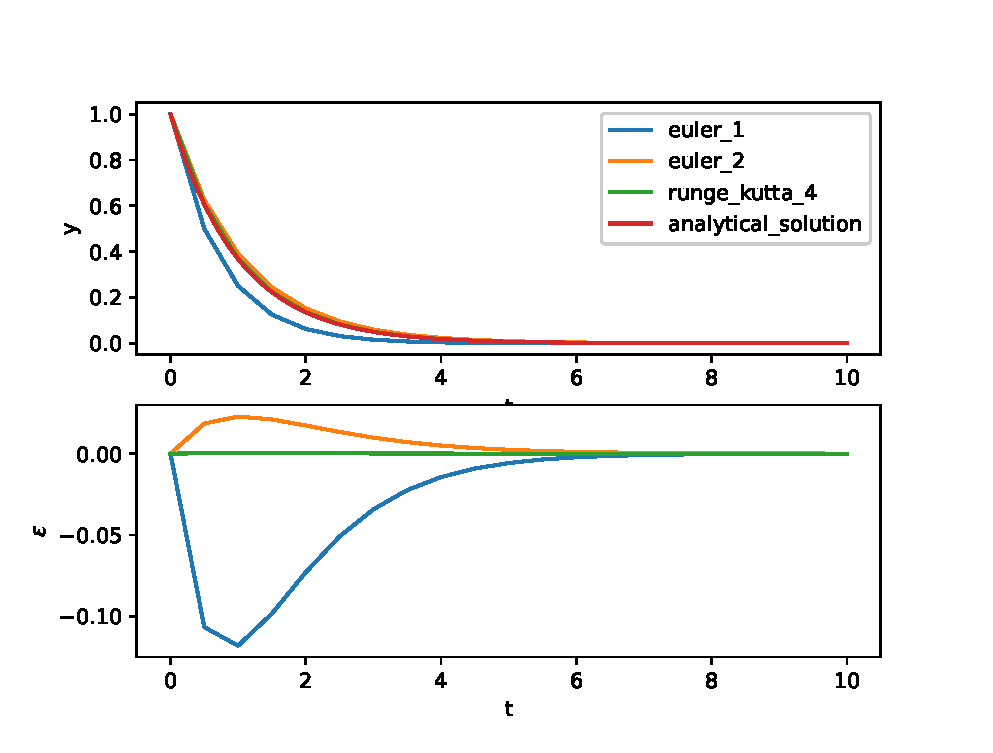
\epsfig{file=relaxation_methods.eps,width=\linewidth}
        \end{subfigure}
        \hfill
        \begin{subfigure}{0.49\linewidth}
            \centering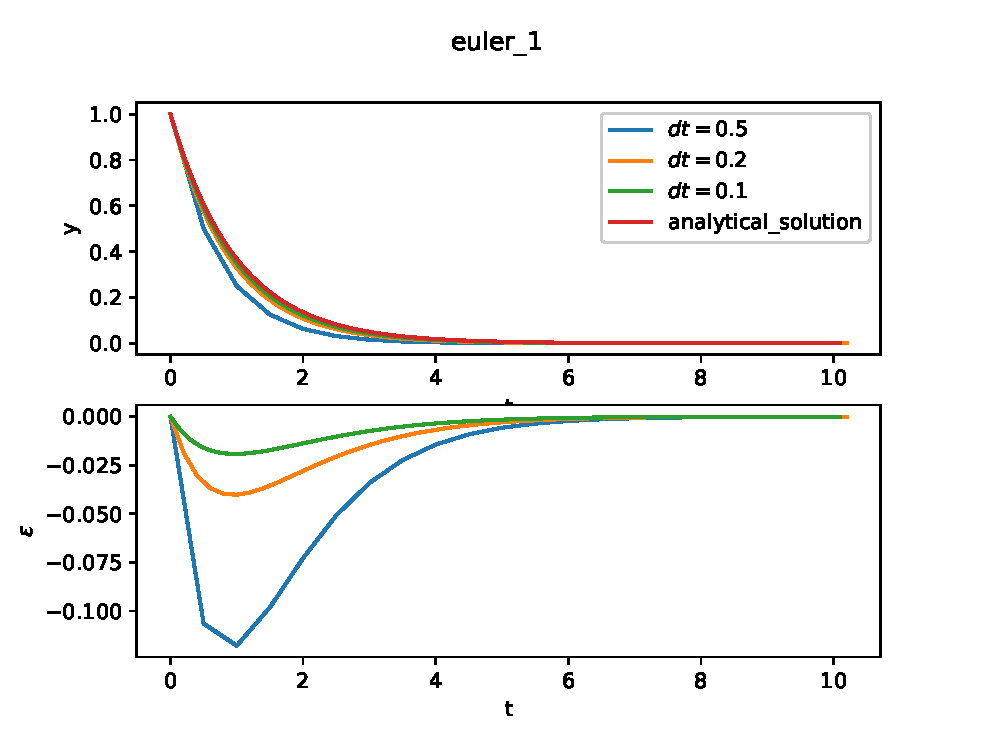
\epsfig{file=relaxation_euler_1.eps,width=\linewidth}
        \end{subfigure}
        \begin{subfigure}{0.49\linewidth}
            \centering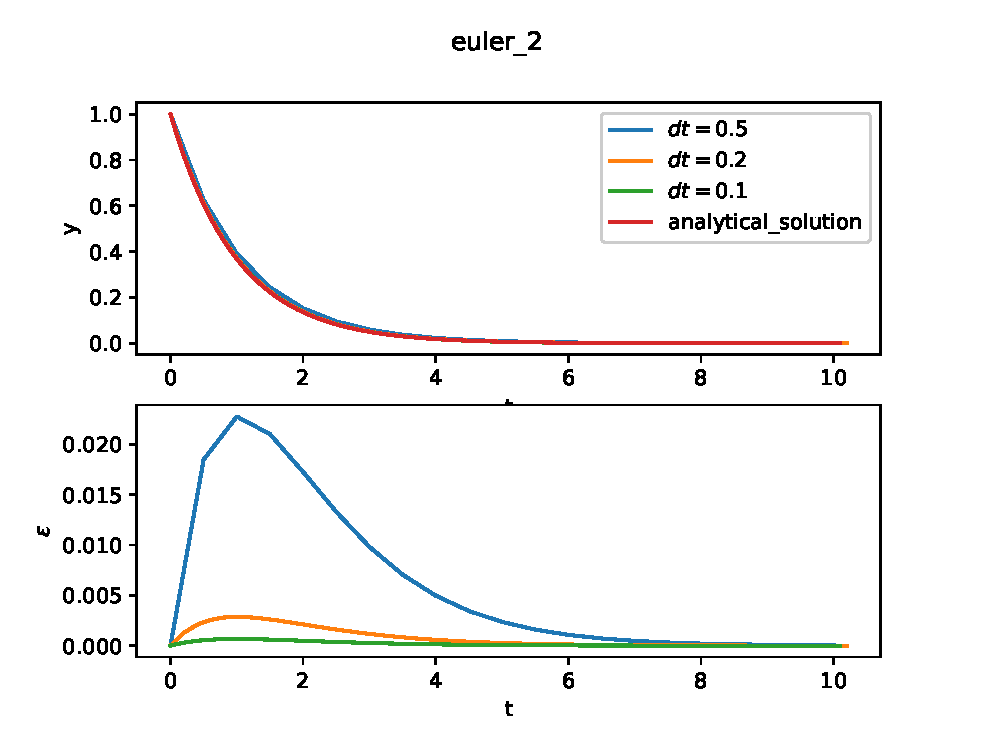
\epsfig{file=relaxation_euler_2.eps,width=\linewidth}
        \end{subfigure}
        \hfill
        \begin{subfigure}{0.49\linewidth}
            \centering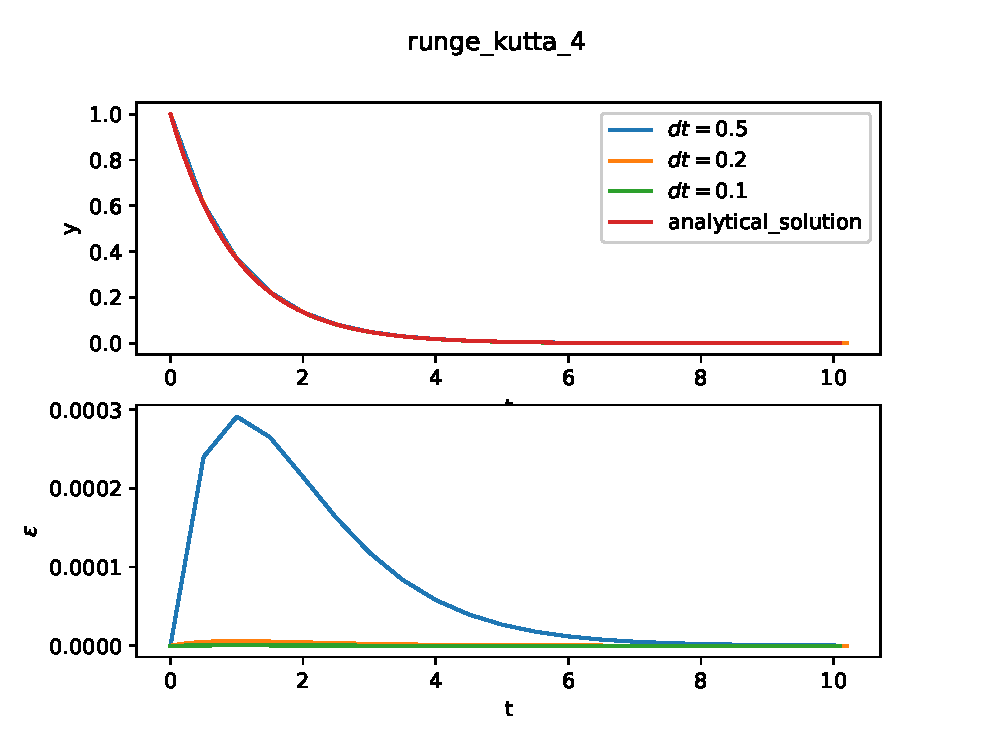
\epsfig{file=relaxation_runge_kutta_4.eps,width=\linewidth}
        \end{subfigure}
        \caption{
            \protect\small
            Integrace relaxační diferenciální rovnice ~\eqref{eq:relaxace} různými metodami a s různými časovými kroky.
        }	
        \label{fig:relaxace}
    \end{figure}

    \begin{itemize}
    \item \ghfile{python/ode/}{ode.py}: 
        Modul napsaný maximálně obecně, aby ho bylo možné použít na řešení libovolné diferenciální rovnice, a také soustav diferenciálních rovnic probíraných v sekci~\ref{sec:ODRn}.
        
        \begin{itemize}
        \item \code{euler_1}: 
            Integrační krok Eulerovy metody 1. řádu.
        \item \code{euler_2}: 
            Integrační krok Eulerovy metody 2. řádu.
        \item \code{runge_kutta_4}: 
            Integrační krok Runge-Kuttovy metody 4. řádu.
        \item \code{ode_solve}: 
            Integruje diferenciální rovnici danou pravou stranou prvního parametru \code{model} s počáteční podmínkou předanou parametrem \code{initial_condition}. 
            Integrační metodu lze specifikovat parametrem \code{integrator}, což je vlastně funkce $\phi(y_{i}, t_{i})$ z rovnice~\eqref{eq:phi}. 
            Délku kroku udává parametr \code{dt}.
            Funkce vrací pole hodnot řešení rovnice (soustavy rovnic) v jednotlivých časech a pole časů.
        \item \code{scipy_ode_solve}: 
            Integruje diferenciální rovnici pomocí funkce \code{odeint} z knihovny \code{sci\-py.integrate}. 
            Pozor, parametr \code{dt} zde neznačí integrační krok, nýbrž časový krok výsledného pole.
            Funkce \code{odeint} používá sofistikovaný řešitel diferenciálních rovnic s proměnným krokem.
            Pro podrobnosti můžete mrknout na \href{https://docs.scipy.org/doc/scipy/reference/generated/scipy.integrate.odeint.html}{dokumentaci} k této funkci.
    \end{itemize}

    \item \ghfile{python/ode/}{graphs.py}: 
        Vykresluje grafy srovnávající různé metody nebo různé kroky výpočtu.
        \begin{itemize}
        \item \code{plot_solution_error}:
            Vykreslí graf řešení diferenciální rovnice.
            Parametr \code{analyti\-cal_solution} je odkaz na přesné řešení dané diferenciální rovnice. 
            Je-li zadán, vykreslí se do grafu dva panely: jeden s hodnotami numerického řešení, druhý s rozdílem řešení numerického a přesného $\epsilon$ (akumulovaná diskretizační chyba dle  rovnice~\eqref{eq:AkumulovanaChyba}).
        \item \code{plot_compare_methods}:
            Vykreslí do jednoho obrázku řešení zadané diferenciální rovnice různými metodami.
            Z důvodu efektivnějšího kódu se v této funkci používá trochu složitější práce s panely, než jak je uvedeno ve vzorovém souboru \ghfile{python/basics/}{plot.py}.
        \item \code{plot_compare_steps}:
            Vykreslí do jednoho obrázku řešení zadané diferenciální rovnice s různými integračními kroky.
        \item \code{plot_cummulative_errors}:
            Řešení úlohy~\ref{task:KumulovanaChyba}.
        \end{itemize}

    \item \file{relaxation.py}:
        Soubor, který využívá integračních funkcí z modulu \ghfile{python/ode/}{ode.py} a vykreslovacích funkcí z modulu \ghfile{python/ode/}{graphs.py}
        pro řešení diferenciální rovnice pro relaxaci.
        \begin{itemize}
        \item Vyřeší diferenciální rovnici různými metodami, řešení nakreslí do jednoho grafu a porovná s teoretickou funkcí.
        \item Vyřeší diferenciální rovnici s různým časovým krokemm, řešení nakreslí do jednoho grafu a porovná s teoretickou funkcí.
        \item Nakreslí graf k úloze~\ref{task:KumulovanaChyba}.
        \end{itemize}
    \end{itemize}

    Příslušné grafy jsou zobrazeny na obrázku~\ref{fig:relaxace}.
    Je vidět, že chyba opravdu klesá s řádem metody a že čím je metoda vyššího řádu, tím rychleji chyba klesá se zmenšujícím se krokem.
\end{solution}

\begin{task}
\label{task:KumulovanaChyba}
    Rozšiřte kód tak, aby počítal průměrnou kumulovanou chybu
    \begin{equation}\label{eq:KumulovanaChyba}
        \mathcal{E}=\sqrt{\frac{1}{n}\sum_{i=0}^{n-1}\left(y_{i}-y(t_{i})\right)^{2}},
    \end{equation}
    kde $y(t)$ je analytické řešení diferenciální rovnice.
    Nakreslete závislost $\mathcal{E}(\Delta t)$ pro $\Delta t\in\langle0.002;0.1\rangle$ a pro různé metody.
    Jelikož očekáváme mocninnou závislost dle~\eqref{eq:RadMetodyODR}, kde exponent je tím větší, čím větší je řád metody, je výhodné graf $\mathcal{E}(\Delta t)$ kreslit v log-log měřítku.
    V Pythonu použijete místo \textnormal{\texttt{plot(...)}} funkci \textnormal{\texttt{loglog(...)}} z knihovny \textnormal{\texttt{matplotlib.pyplot}}.
    Ověřte, že získané křivky jsou v souladu s řády použitých metod.
\end{task}

\begin{solution}
    \begin{figure}[!htb]
        \centering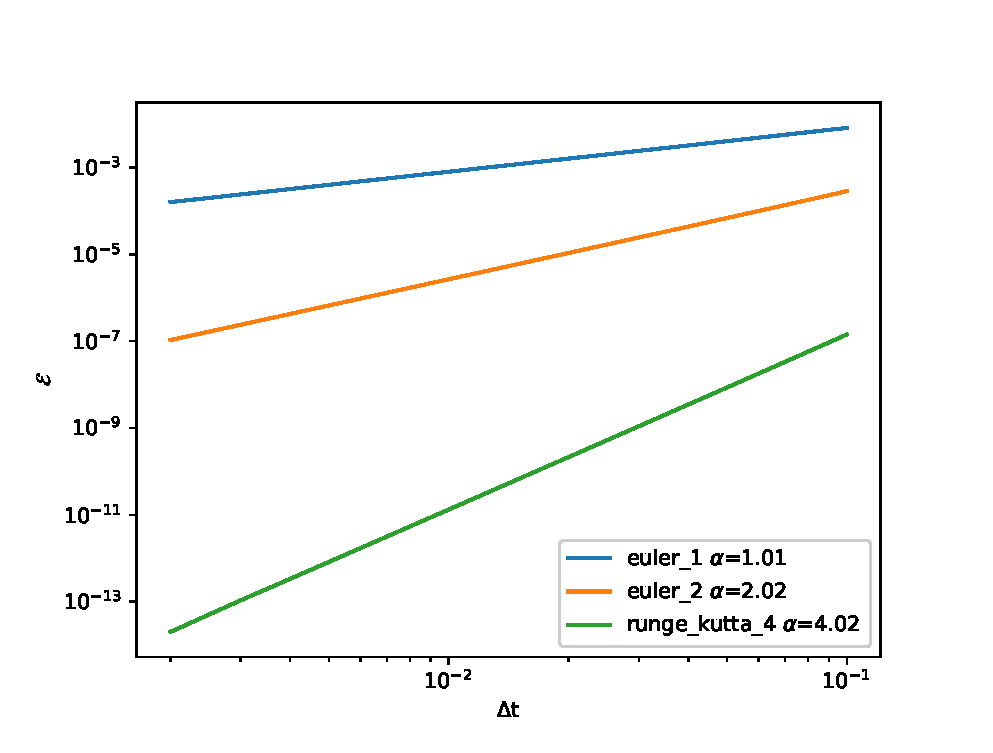
\epsfig{file=relaxation_cummulative_error.eps,width=0.7\linewidth}
        \caption{
            \protect\small
            Závislost průměrné kumulované chyby~\eqref{eq:KumulovanaChyba} na délce kroku $\Delta t$ vypočítaná a vykreslená pomocí funkce pro relaxační diferenciální rovnici.
        }
        \label{fig:relaxace_chyba}
    \end{figure}

    Řešení této úlohy vykreslí funkce \code{plot_cummulative_error} z modulu \ghfile{python/ode/}{graphs.py}. Graf je zobrazen na obrázku~\ref{fig:relaxace_chyba}.
    Body log-log grafu byla proložena přímka pomocí funkce lineární regrese \code{linregress} z knihovny \file{scipy.stats}.
    Nafitovaná směrnice $\alpha$ je uvedena v obrázku.
\end{solution}


\begin{task}
    Pomocí naprogramovaných metod vyřešte nelineární diferenciální rovnici
    \begin{equation}
        \label{eq:sinyt}
        \derivative{y}{t}=\sin\left(t y\right)
    \end{equation}
    s počáteční podmínkou $y_{0}=1$, $t_{0}=0$ a vykreslete graf jejího řešení.
\end{task}

\begin{solution}
    \begin{figure}[!htb]
        \centering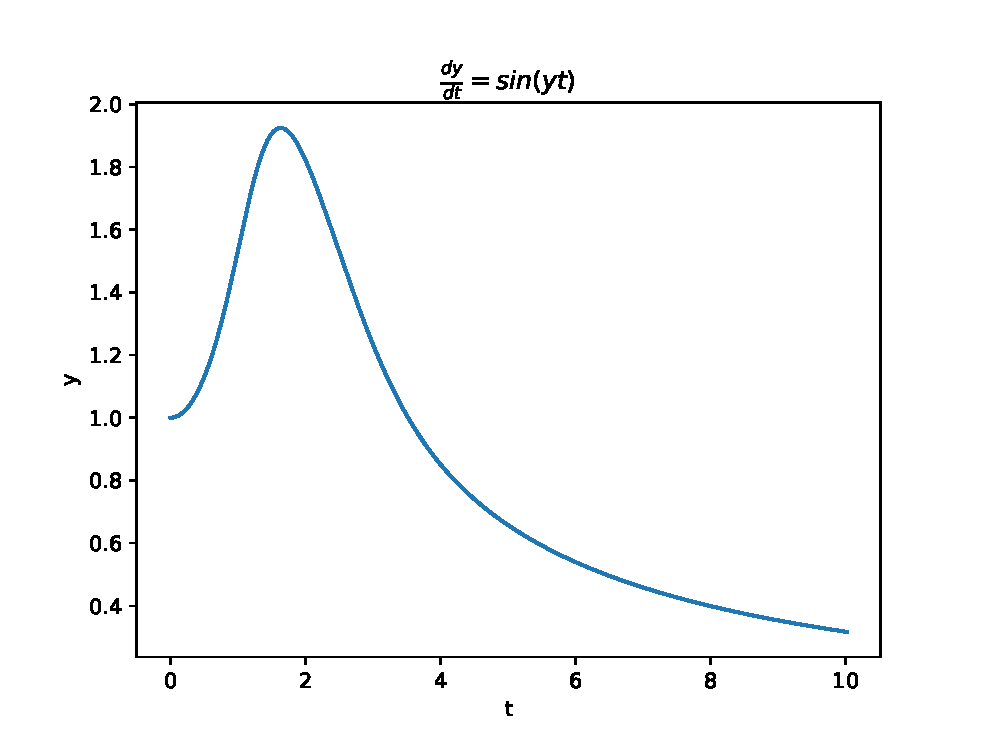
\epsfig{file=sinyt.eps,width=0.7\linewidth}
        \caption{
            \protect\small
            Řešení diferenciální rovnice~\eqref{eq:sinyt} s počáteční podmínkou $y(0)=1$.
            Použitá metoda: Runge-Kutta, časový krok $\Delta t=0.02$.
        }
        \label{fig:sinyt}
    \end{figure}

    Řešení je v souboru \ghfile{python/ode/}{sinyt.py}.
    Graf vypočítané funkce je na obrázku~\ref{fig:sinyt}.
\end{solution}


\section{Soustavy diferenciálních rovnic 1. řádu}
\label{sec:ODRn}
    Každou obyčejnou diferenciální rovnici $n$-tého řádu lineární v nejvyšší derivaci lze převést na~soustavu $n$ obyčejných diferenciálních rovnic prvního řádu ve tvaru
    \begin{equation}\label{eq:ODR}
        \derivative{\vector{y}}{t}=\vector{f}(\vector{y},t),
    \end{equation}
    kde $\vector{y}=\vector{y}(t)$ je vektor hledaných funkcí a $\vector{y}(t_{0})=\vector{y}_{0}$ vektor počáteční podmínky.

    \begin{example}
        Pohybovou rovnici
        \begin{equation}
            Ma=F(x),
        \end{equation}
        kde $M$ je hmotnost pohybujícího se tělesa, $x=x(t)$ jeho poloha a $a=a(t)=\d^{2}x/\d t^{2}$ zrychlení převedeme na~dvě diferenciální rovnice prvního řádu zavedením rychlosti $v=v(t)=\d x/\d t$:\footnote{
            Tato soustava rovnic odpovídá Hamiltonovým pohybovým rovnicím, se kterými se seznámíte v přednášce Teoretická mechanika.
        }
        \begin{equation}
            \derivative{}{t}\makematrix{x \\ v}=\makematrix{v \\ \frac{1}{M}F(x)},
        \end{equation}
        tj. vektor funkce pravých stran podle rovnice~\eqref{eq:ODR} je
        \begin{equation}
            \vector{f}(\vector{y},t)=\makematrix{v \\ \frac{1}{M}F(x)}
        \end{equation}
        kde $\vector{y}\equiv\makematrix{x \\ v}$.
    \end{example}

    \begin{example}
    Pohybová rovnice pro harmonický oscilátor (matematické kyvadlo s malou výchylkou) při volbě jednotek $M=\Omega=1$, kde $M$ je hmotnost kmitající částice a $\Omega$ její rychlost, zní
    \begin{align}
        a&=\derivative[2]{x}{t}=-x &&\Longleftrightarrow &
        \derivative{}{t}\makematrix{x \\ v}&=\makematrix{v \\ -x}
    \end{align}

    \end{example}

    \begin{voluntary}
    Převeďte na soustavu obyčejných diferenciálních rovnic prvního řádu rovnici třetího řádu pro Hiemenzův tok
    \begin{equation}
        x'''+xx''-x'^{2}+1=0.
    \end{equation}
    \end{voluntary}

    \begin{solution}
    Hledaná soustava diferenciálních rovnic je
    \begin{equation}
        \derivative{}{t}\makematrix{x \\ v \\ a}=\makematrix{v \\ a \\ -xa+v^{2}-1}.
    \end{equation}
    \end{solution}

    Drtivá většina knihoven a algoritmů pro integraci obyčejných diferenciálních rovnic počítá s rovnicemi ve~tvaru~\eqref{eq:ODR}.

\subsection{Symplektické algoritmy}
    Jedná se o speciální algoritmy navržené pro řešení pohybových differenciálních rovnic.
    Od běžných algoritmů je odlišuje to, že zachovávají objem fázového prostoru, a~tedy i energii (zatímco u obecných algoritmů se energie s integračním časem mění a většinou roste).
    
    V praxi se ze~symplektických algoritmů používá nejčastěji \emph{Verletův algoritmus}.
    Pro diferenciální rovnici 2. řádu ve tvaru 
    \begin{equation}\label{eq:EM}
        M\derivative[2]{x}{t}=F(x),
    \end{equation}
    což je pohybová rovnice pro jeden hmotný bod o hmotnosti $M$, na který působí časově neproměnná síla $F(x)$, má Verletův algoritmus tvar
    \begin{align}
        x_{i+1}&=x_{i}+v_{i}\Delta t+\frac{1}{2}a_{i}\Delta t^{2},\nonumber\\
        v_{i+1}&=v_{i}+\frac{1}{2}\left(a_{i+1}+a_{i}\right)\Delta t,
        \label{eq:Verlet}
    \end{align}
    kde $a_{i}\equiv F(x_{i})/M$ je zrychlení částice.

    Verletův algoritmus se používá nejčastěji v molekulární dynamice k simulaci pohybu velkého množství vzájemně interagujících částic.
    Jedná se o velmi rychlou a efektivní metodu.

    Řád Verletova algoritmu je $p=2$. 
    Symplektické algoritmy s vyšším řádem existují, avšak v praxi se nepoužívají.

\newpage
{\color{red}\subsection{Domácí úkol na 30.3.2021}}
\begin{task}
    Rozšiřte kód naprogramovaný v úkolu~\ref{task:ODR1} tak, aby fungoval pro libovolně velkou soustavu obyčejných diferenciálních rovnic.
    Využijte k tomu funkce pro práci s řadami z knihovny \file{numpy} popsané v sekci~\ref{sec:numpy}.
    Vyřešte diferenciální rovnici harmonického oscilátoru 
    \begin{equation}\label{eq:HO}
        \derivative[2]{x}{t}=-x
    \end{equation}
    s počátečními podmínkami $x_{0}=0$, $x'_{0}\equiv v_{0}=1$, $t_{0}=0$ a porovnejte řešení různými metodami s analytickým řešením $x(t)=\sin t$.
    Jako časový krok volte například $\Delta t=0.1$ a $\Delta t=0.01$ a počítejte na časovém intervalu $t\in\langle 0;30\rangle$.
\end{task}    

\begin{solution}
\label{sol:ODRn}
    Metody jsou naprogramovány v souborech \ghfile{python/ode/}{ode.py} (integrační metoda), \ghfile{python/ode/}{graphs.py} (vykreslování grafů) a jsou podrobně diskutování v řešení úlohy~\ref{sol:ODR1}.
    Soubor \ghfile{python/ode/}{ho.py} obsahuje pravé strany diferenciálních rovnic harmonického oscilátoru (funkce \code{ho}) a volá všechny výpočetní a vykreslovací funkce.
    Navíc obsahuje následující funkce:
    \begin{itemize}
    \item \code{ho_solution}:
        Přesné řešení pohybové rovnice harmonického oscilátoru s počáteční podmínkou $x_{0}=0,x'_{0}=1,t_{0}=0$, jímž je funkce $x(t)=\sin t$.
    \item \code{ho_energy}:
        Pro vstupní polohu a rychlost (nebo pole poloh a rychlostí) vrátí energii harmonického oscilátoru.
    \end{itemize}

    \begin{figure}[!htb]
        \begin{subfigure}{0.49\linewidth}
            \centering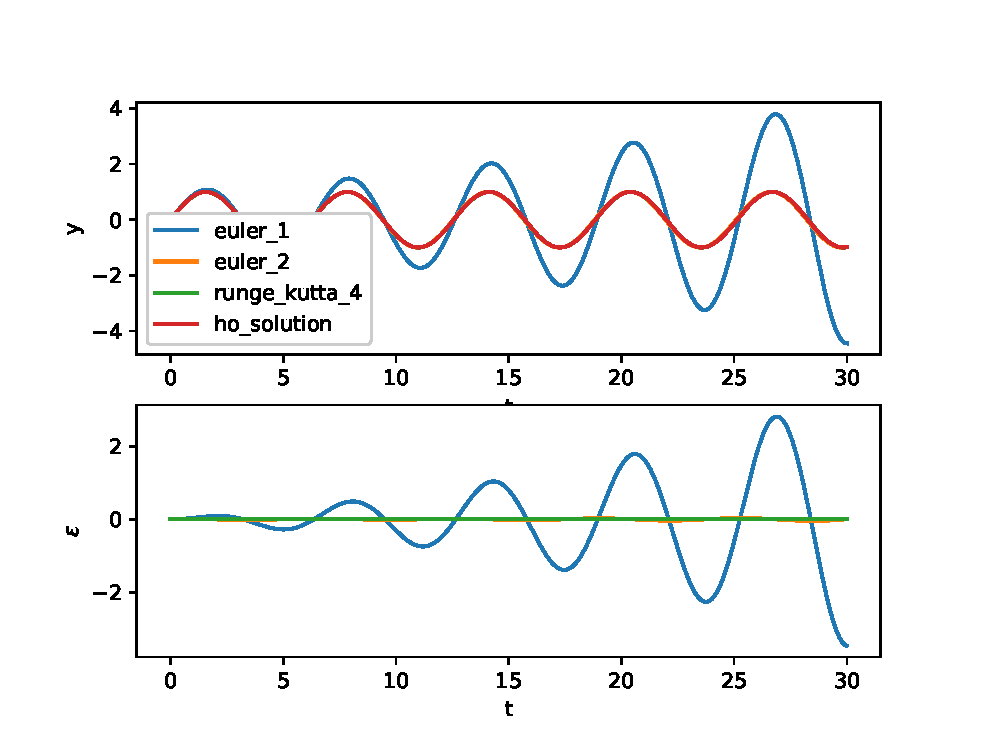
\epsfig{file=ho_methods.eps,width=\linewidth}
        \end{subfigure}
        \hfill
        \begin{subfigure}{0.49\linewidth}
            \centering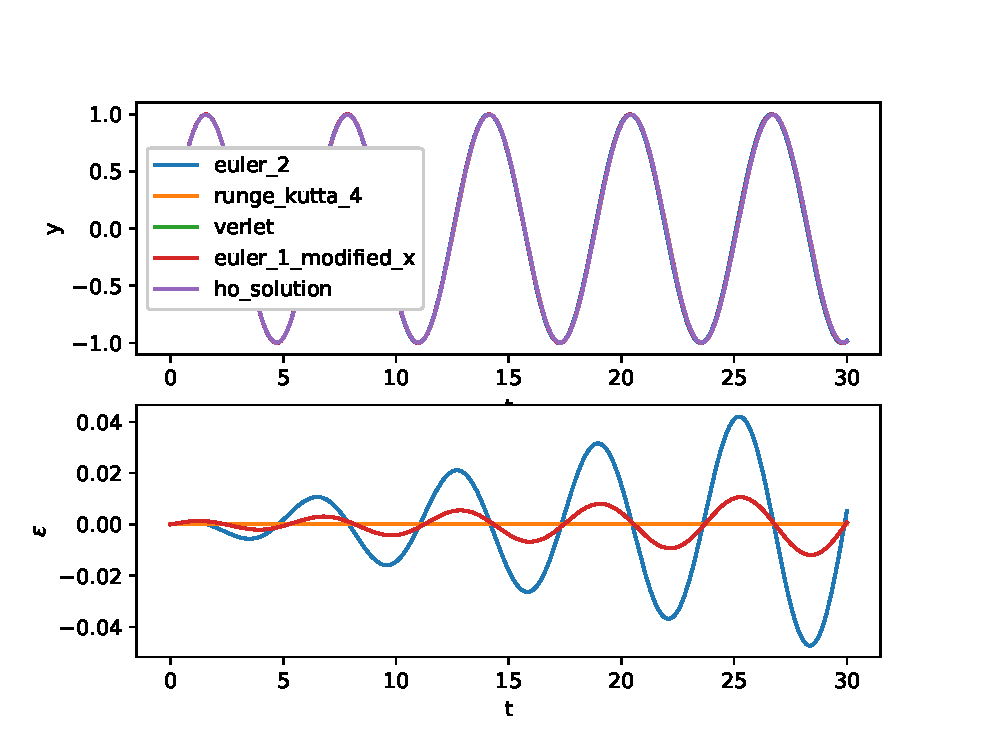
\epsfig{file=ho_symplectic.eps,width=\linewidth}
        \end{subfigure}
        \begin{subfigure}{0.49\linewidth}
            \centering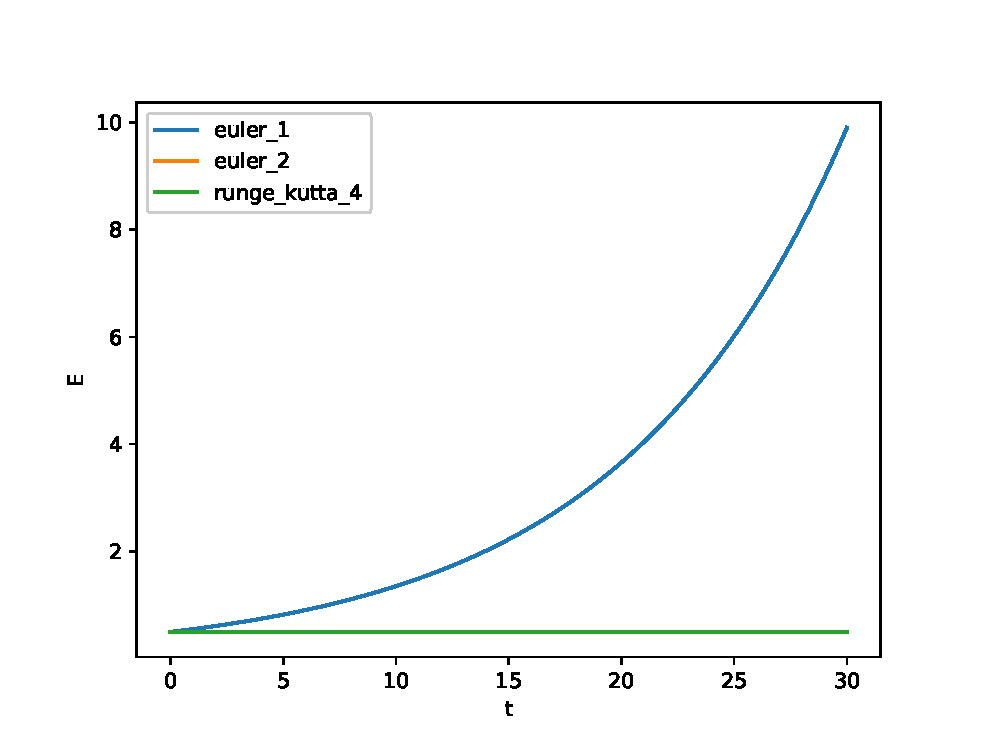
\epsfig{file=ho_energy.eps,width=\linewidth}
        \end{subfigure}
        \hfill
        \begin{subfigure}{0.49\linewidth}
            \centering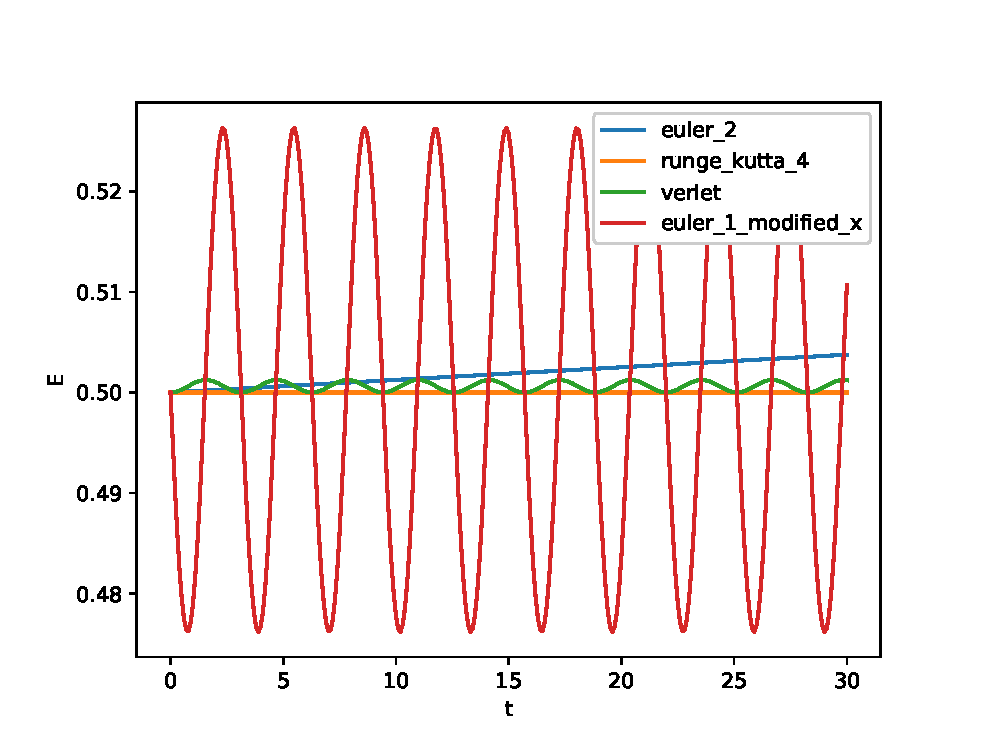
\epsfig{file=ho_energy_symplectic.eps,width=\linewidth}
        \end{subfigure}
        \caption{
            \protect\small
            Integrace diferenciální rovnice harmonického oscilátoru~\eqref{eq:HO} různými metodami.
            Časový krok je $\Delta t=0.1$.
            \emph{Levý sloupec:} všechny metody.
            \emph{Pravý sloupec:} Bez eulerovy metody 1. řádu a včetně symplektických metod.
            \emph{1.~řádek:} hodnoty $y(t)$.
            \emph{2.~řádek:} Akumulované diskretizační chyby dle~\eqref{eq:AkumulovanaChyba}.
            Pro Eulerovu metodu 1. řádu je obalová křivka divergence numerického od analytického řešení očividně exponenciální v čase.
            \emph{3.~řádek:} energie~\eqref{eq:HOE}. 
            Pro Eulerovy metody energie roste.
            Energie se mění i pro Runge-Kuttovu metodu (pro tento systém energie s časem klesá), avšak změna je řádově menší než pro ostatní metody, a tudíž není na grafech při daném měřítku svislé osy vidět.
            Naopak pro Verletův algoritmus a pro \uv{předbíhající} Eulerovu metodu energie osciluje okolo počáteční energie $E=\frac{1}{2}$.
        }	
        \label{fig:HO}
    \end{figure}

    Příslušné grafy jsou zobrazeny na obrázku~\ref{fig:HO}.
\end{solution}


\begin{task}
    Naprogramujte Verletův algoritmus~\eqref{eq:Verlet}.
    Ukažte, že zatímco při použití Eulerovy metody nebo Runge-Kuttovy metody energie systému v průběhu výpočtu roste, Verletův algoritmus energii zachovává.
    Energie bezrozměrného harmonického oscilátoru~\eqref{eq:HO} je dána vzorcem
    \begin{equation}\label{eq:HOE}
        E=\frac{1}{2}\left(x^{2}+v^{2}\right).
    \end{equation}
\end{task}

\begin{solution}
    Symplektický Verletův algoritmus je naprogramován v souboru \ghfile{python/ode/}{symplectic.py}.
    Toto vzorové řešení bude fungovat \emph{jen} pro jednu pohybovou rovnici, tj. pro jednu diferencální rovnici původně druhého řádu přepsanou na dvě diferenciální rovnice prvního řádu, přičemž první rovnice musí být pro souřadnici, druhá pro rychlost. 
    Řešení lze samozřejmě rozšířit na více pohybových rovnic.

    V souboru \ghfile{python/ode/}{symplectic.py} je i funkce \code{plot_energy}, která vykreslí graf závislosti $E(t)$.
    Energie je znázorněna v panelech na třetím řádku na obrázku~\ref{fig:HO}.
    Harmonický oscilátor je konzervativní systém (zachovává energii), pozorovaná rostoucí energie je způsobena nepřesností integračních metod.
    U symplektických algoritmů energie slabě osciluje okolo střední hodnoty, která však i pro velmi dlouhé časy zůstává na přesné hodnotě $E=\frac{1}{2}$.
\end{solution}


\begin{task}
    Eulerovu metodu 1. řádu lze pro soustavy dvou diferenciálních rovnic 1. řádu vylepšit následující záměnou:
    \begin{align}
        &\begin{matrix}
            x_{i+1}=x_{i}+v_{i}\Delta t \\
            v_{i+1}=v_{i}-x_{i}\Delta t 
        \end{matrix}
        &&\longrightarrow
        &\begin{matrix}
            x_{i+1}=x_{i}+v_{i}\Delta t \\
            v_{i+1}=v_{i}-x_{i+1}\Delta t 
        \end{matrix}
    \end{align}
    (vypočítáme $x_{i+1}$ a tuto hodnotu použijeme namísto hodnoty $x_{i}$ pro výpočet rychlosti $v_{i+1}$).
    Naprogramujte tuto metodu a pomocí výsledků úlohy~\ref{task:KumulovanaChyba} ukažte, že pro harmonický oscilátor se jedná o metodu 2. řádu.
\end{task}

\begin{solution}
    \uv{Vylepšené} Eulerovy metody jsou naprogramovány v souboru \ghfile{python/ode/}{symplectic.py}.
    Metoda s předbíhající se souřadnicí je označena \code{euler_1_modified_x}, metoda s předbíhající rychlostí pak \code{euler_1_modified_v}.
    Obě metody dávají velmi podobné výsledky, v grafech je proto uvedena jen první z nich.

    Řešení diferenciální rovnice harmonického osciátoru je znázorněno v pravém sloupci obrázku~\ref{fig:HO}.
    Je vidět, že so se přesnosti týče, vylepšená Eulerova metoda je srovnatelná s Verletovou metodou.
    Energie však osciluje trochu víc.

    \begin{figure}[!htbp]
        \centering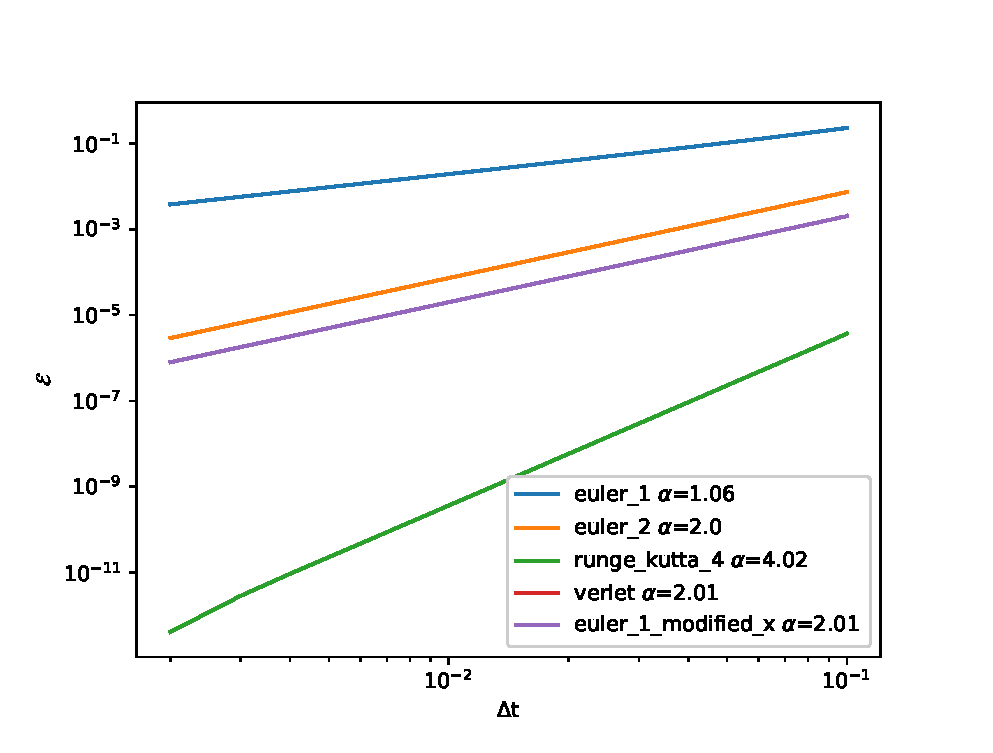
\epsfig{file=ho_cummulative_error.eps,width=0.7\linewidth}
        \caption{
            \protect\small
            Závislost průměrné kumulované chyby~\eqref{eq:KumulovanaChyba} na délce kroku $\Delta t$ vypočítaná a vykreslená pro soustavu diferenciálních rovnic pro harmonický osciátor.
            Zobrazeny jsou i symplektické metody.
        }
        \label{fig:ho_chyba}
    \end{figure}
    
    Řád metody lze určit na základě obrázku~\ref{fig:ho_chyba}.
    Jak u Verletovy metody, tak u vylepšené Eulerovy metody klesá průměrná kumulovaná chyba s druhou mocninou délky časového kroku $\delta t$, jedná se tedy o metody 2. řádu.
\end{solution}


\begin{task}
    Pohrajte si s řešením rovnice pro klesající exponenciálu
    \begin{equation}\label{eq:Exp2}
        \derivative[2]{x}{t}=x
    \end{equation}
    s počátečními podmínkami $x_{0}=1$, $x'_{0}=-1$.
    Přesvědčte se, že Verletova metoda a vylepšená Eulerova metoda z předchozího úkolu jsou nestabilní --- pro tuto rovnici v relativně krátkém čase začnou řešení exponenciálně divergovat.
\end{task}

\begin{solution}
    Řešení rovnice~\eqref{eq:Exp2} je v souboru \ghfile{python/ode/}{exp.py}.
    Soustava rovnic je analogická k soustavě harmonického oscilátoru --- liší se pouze znaménkem.
    Systém popsaný touto rovnicí \emph{není konzervativní} --- nelze nadefinovat zachovávající se veličinu, která by měla význam energie.

    \begin{figure}[!htbp]
        \centering
        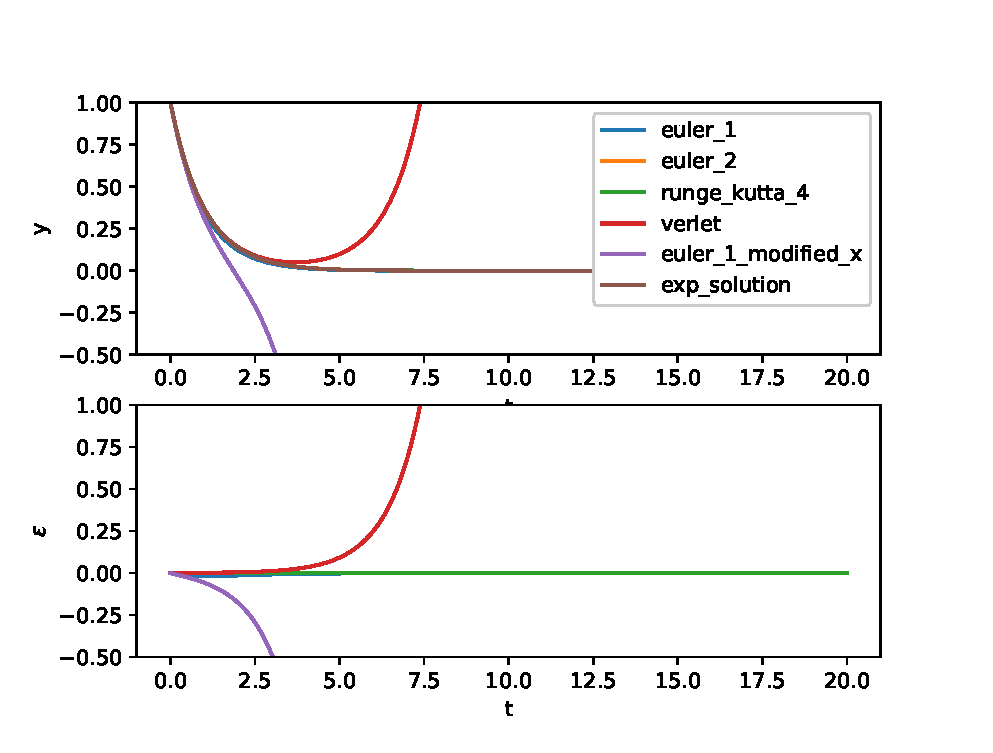
\epsfig{file=exp_divergence.eps,width=0.8\linewidth,keepaspectratio}
        \caption{
            \protect\small
            Totéž jako v obrázku~\ref{fig:HO}, avšak pro exponenciálně klesající systém daný rovnicí~\eqref{eq:Exp2}.
            Symplektické algoritmy jsou nestabilní.
            }	
        \label{fig:Exp2}
    \end{figure}
    
    Z obrázku~\ref{fig:Exp2} je vidět, že symplektické algoritmy jsou nestabilní, a tudíž nejsou na tento typ úlohy vhodné, což je pochopitelné, protože jsou navrženy pouze pro energii zachovávající systémy.
    Příčinu nestability lze nahlédnout i z obecného řešení rovnice~\eqref{eq:Exp2},
    \begin{equation}
        y(t)=A\e^{t}+B\e^{-t},
    \end{equation}
    přičemž my speciálními počátečními podmínkami vybíráme pouze exponenciálně klesající řešení.
    Symplektické algoritmy však v určitou chvíli \uv{překmitnou} na exponenciálně rostoucí řešení, což způsobí pozorovanou divergovat.
\end{solution}

\begin{task}
    Vyřešte nelineární soustavu tří diferenciálních rovnic pro jednoduchý Lorenzův model vedení tepla v atmosféře
    \begin{align}
        \derivative{x}{t}&=\sigma(y-x),\nonumber\\
        \label{eq:Lorenz}
        \derivative{y}{t}&=x(\rho-z)-y,\\
        \derivative{z}{t}&=xy-\beta z\nonumber
    \end{align}
    s hodnotami parametrů $\sigma=10$, $\rho=28$ a $\beta=8/3$, počátečními podmínkami $(x_0, y_0, z_0)=(1,1,1)$ (na počátečních podmínkách zase tolik nezáleží), s krokem $\Delta t=0.01$ a na časovém intervalu $t\in\langle0,100\rangle$.
    Vykreslete graf $z(x)$.
    Výsledná křivka je slavný Lorenzův podivný atraktor ve tvaru motýlích křídel, krerý zpopularizoval teorii klasického chaosu.
\end{task}

\begin{solution}
    Řešení Lorenzova systému diferenciálních rovnic je jednoduchou aplikací kódu naprogramovaného v úloze~\ref{sol:ODRn} a lze ho nalézt v souboru \ghfile{python/ode/}{lorenz.py}.
    Příslušnou projekci trojrozměrné trajektorie do 2D roviny $(x,z)$ lze nalézt na obrázku~\ref{fig:Lorenz}.

    \begin{figure}[!htbp]
        \centering
        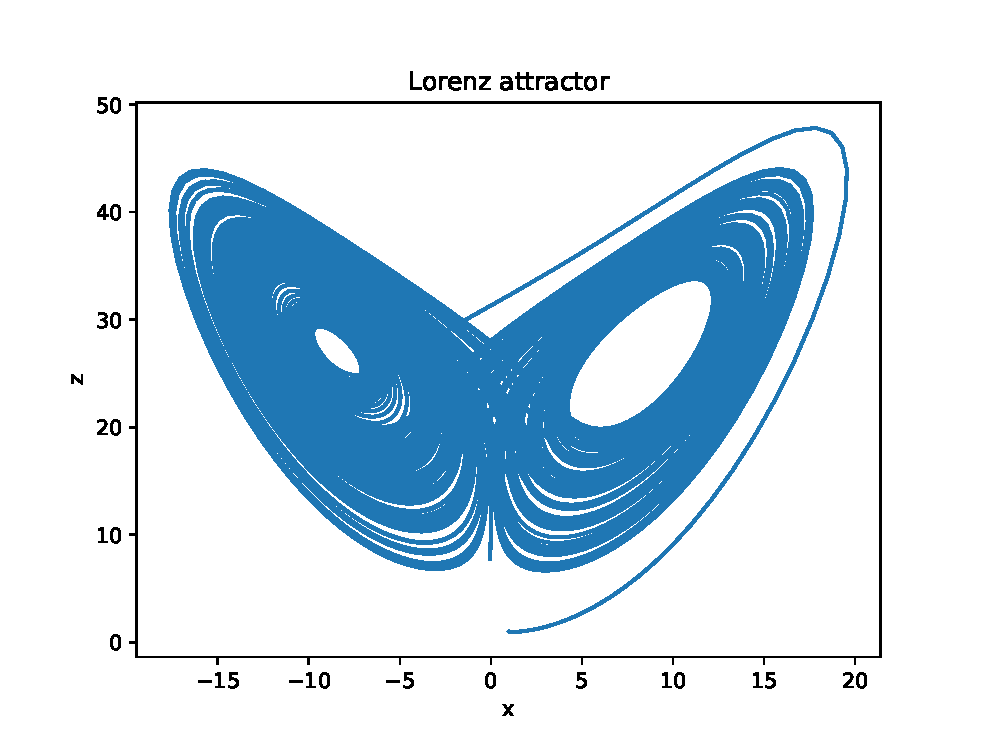
\epsfig{file=lorenz.eps,width=0.7\linewidth,keepaspectratio}
        \caption{
            \protect\small
                Lorenzův systém~\eqref{eq:Lorenz} integrovaný pomocí Runge-Kuttovy metody 4. řádu na časovém intervalu $t\in\langle0;100\rangle$ s krokem $\Delta t=0.01$.
            }	
        \label{fig:Lorenz}
    \end{figure}
\end{solution}

\subsection{Shrnutí}
\begin{itemize}
\item 
    Řešitelé obyčejných diferenciálních rovnic převážně pracují se soustavami diferenciálních rovnic prvního řádu.
    Na tento tvar není obtížné diferenciální rovnici vyššího řádu převést.

\item
    Nejčastěji se používají jednokrokové metody, jejichž hlavní výhoda je v možnosti jednoduše dle potřeby měnit délku kroku (metody s adaptivním krokem).

\item 
    Přesnost řešení závisí na řádu metody $p$ a na délce integračního kroku $\Delta t$.
    Čím je řád metody vyšší, tím rychleji klesá chyba se zmenšujícícm se krokem.
    V praxi, pokud nechcete svěřit svůj probém černé skříňce ve formě nějaké hotové knihovny, se velmi často používá Runge-Kuttova metoda 4. řádu, která je jednoduchá na implementaci, je stabilní a rychlá.

\item
    Symplektické metody, z nichž nejběžnější je Verletova metoda, jsou výhodné k modelování fyzikálních systémů zachovávajících energii.
    Pro nekonzervativní systémy nejsou vhodné. 
\end{itemize}
A hlavně, nyní již umíte jen pomocí sčítání a násobení vypočítat a nakreslit průběh goniometrické funkce sinus.


\section{Náhodná procházka}\label{sec:NahodnaProchazka}
    Náhodná procházka je jeden ze základních prostředků, jak simulovat velké množství nejen fyzikálních procesů (například pohyb Brownovské částice, fluktuace akciového trhu, cestu opilce z~hospody atd.).
    V dalších cvičeních si ukážeme, jak se pomocí náhodné procházky dá jednoduše hledat minimum funkcí (a to i funkcí více proměnných). 

    Algoritmus pro náhodnou procházku je následující: v každém časovém kroku uděláme krok v~$d$-rozměrném prostoru $\vector{y}_{i}\rightarrow\vector{y}_{i+1}$ takovým způsobem, aby pravděpodobnost pohybu do všech směrů byla stejná.
    Délka kroku $s$ se volí buď náhodná, nebo konstantní.

    K simulování náhodných procesů slouží algoritmy generující pseudonáhodná čísla, což jsou čísla, která mají statistické vlastnosti blízké vlastnostem skutečných náhodných čísel, avšak jsou počítána jednoduchými deterministickými algoritmy.
    Náhodná čísla se generují od počáteční tzv. \emph{násady} (seed), kterou lze explicitně zadat, a tím posloupnost náhodných čísel přesně zreprodukovat (díky tomu, že generující algoritmy jsou deterministické).
    Pokud násada není explicitně zadána, knihovny pro generování pseudonáhodných čísel většinou volí systémový čas, takže při každém spuštění programu dostáváme posloupnost odlišnou.

    Základní funkce a postupy pro generování náhodných čísel v Pythonu jsou uvedeny v sekci~\ref{sec:PseudonahodnaCisla}.

    {\color{red}\subsection{Domácí úkol na 6.4.2021}}
    \begin{task}
        Naprogramujte náhodnou procházku ve 2D rovině.
        Délku kroku volte konstantní $s=1$, směr volte náhodně.
        Začněte z bodu $(x,y)=(0,0)$ a procházku ukončete poté, co opustíte oblast tvaru čtverce o hraně délky $2a$.
        Uchovávejte celou procházku v poli či seznamu.
        Nakonec trajektorii vykreslete do~grafu.
    \end{task}

    \begin{solution}
        Řešení je naprogramováno v souboru \ghfile{python/randomwalk/}{2d.py}.
        \begin{itemize}
            \item \code{random_direction_2d} vrátí náhodný směr ve 2D rovině [generuje náhodný úhel $\phi$, směr je dán jednotkovým vektorem se složkami $(\cos\phi,\sin\phi)$].
            \item \code{random_walk_2d} vykreslí do grafu náhodnou procházku s \code{num_steps} kroky omezenou ve čtverci rozměru $2*$\code{box_size}$\times2*$\code{box_size} a náhodnou procházku vrátí.
            \item \code{random_walk_2d_interactive} generuje náhodnou procházku a vykresluje ji do grafu krok po kroku.
                Musí být zapnutý interaktivní mód vykreslování \code{plt.ion()} a v prostředí Spyder vypnuto použítí inline grafů příkazem \code{\%matplotlib auto} v konzoli REPL.
                Tato funkce implementuje i cyklické okrajové podmínky.
        \end{itemize}
        Vzorový kód je napsán takovým způsobem, aby mohl být přímočaře rozšířen pro vícerozměrnou náhodnou procházku.
    \end{solution}
    
    \begin{task}
        Upravte náhodnou procházku tak, aby počítala s cyklickými okrajovými podmínkami.
        To znamená, že pokud opustíte oblast čtverce jednou jeho stranou, objevíte se na straně protilehlé (jako kdybyste okraje čtverce zavinuli a slepili).
        Výpočet ukončete poté, co uděláte $n$ kroků.
    \end{task}

    \begin{solution}
        Cyklické okrajové podmínky jsou naprogramovány ve funkci \code{random_walk_2d_inter\-active} v souboru \ghfile{python/randomwalk/}{2d.py}.
        Stejně je lze naprogramovat i do funkce \code{random_walk_2d}, výsledný graf však nebude vypadat příliš hezky.
    \end{solution}

    \begin{task}\label{task:NahodnaProchazka}
        Zamyslete se nad tím, jak byste realizovali náhodnou procházku s konstantní délkou kroku v $d>2$ rozměrech, a zkuste své řešení naprogramovat.
        Zásadní je dodržet požadavek, aby pohyb do jakéhokoliv směru nastával se stejnou pravděpodobností (esence úlohy tedy spočívá v generování náhodného směru v $d$-rozměrném prostoru).
    \end{task}

    \begin{solution}
        Zatímco pro směr ve 2D rovině stačí náhodě generovat jeden úhel (předchozí úloha), vícerozměrné úlohy jsou komplikovanější.
        Přímé rozšíření 2D případu do 3D (či do vyšších dimenzí) za generování více úhlů a použití (hyper-)sférických souřadnic k cíli nevede --- takto otrocky generované směry upřednostňují okolí pólů před rovníkem (rozmyslete).
        K úspěšnému generování náhodného kroku je nutné využít jeden z následujících algoritmů:
        \begin{enumerate}
            \item Hyperkoule vepsaná v hyperkrychli.
                \begin{enumerate}
                    \item Nagenerujeme bod v hyperkrychli o hraně délky $2$, tj. generujeme vektor $\vector{v}$ s $d$ složkami, přičemž každá složka je náhodné číslo z rovnoměrného rozdělení $(-1,1)$.
                    \item Zkontrolujeme, zda bod leží uvnitř vepsané jednotkové koule například tak, že spočítáme jeho normu $v=\abs{\vector{v}}$ a porovnáme, zda $n\leq1$.
                    \item Pokud ne, opakujeme postup od začátku.
                        Pokud ano, nagenerovaný bod promítneme na~jednotkovou kouli (jinými slovy vektor $\vector{v}$ nanormujeme) a získaný jednotkový vektor $\vector{\hat{v}}\equiv\vector{v}/v$ udává hledaný směr. 
                \end{enumerate}
                Tato metoda je nesmírně neefektivní, pokud je dimenze $d$ vysoká, poněvadž v tom případě většina nagenerovaných bodů leží vně vepsané hyperkoule a je zahozena.
                Poměr celkového počtu nagenerovaných bodů ku úspěšným zásahům vnitřku hyperkoule lze snadno spočítat.
                Objem hyperkrychle o hraně délky $2$ je
                \begin{equation}
                    V_{d}^{(\text{krychle})}=2^{d},
                \end{equation}
                objem vepsané hyperkoule o poloměru $1$ je
                \begin{equation}
                    V_{d}^{(\text{koule})}=\frac{\pi^{\frac{d}{2}}}{\Gamma\left(\frac{d}{2}+1\right)},
                \end{equation}
                kde $\Gamma$ je Eulerova gama funkce.
                Vzájemný poměr
                \begin{equation}
                    \eta_{d}\equiv\frac{V_{d}^{(\text{krychle})}}{V_{d}^{(\text{koule})}}=\left(\frac{2}{\sqrt{\pi}}\right)^{d}\Gamma\left(\frac{d}{2}+1\right)
                \end{equation}
                udává, kolik bodů musíme průměrně nagenerovat, abychom se trefili do hyperkoule (reciproká hodnota $1/\eta_{d}$ určuje pravděpodobnost, že se do hyperkoule trefíme).
                Zatímco pro $d=3$ je $\eta_{3}\approx1.91$, pro $d=10$ již $\eta_{10}\approx401$, tj. pro nalezení jednoho náhodného směru v desetirozměrném prostoru musíme nagenerovat v průměru přes $4000$ náhodných čísel.
                Z posledního vztahu je vidět, že s rostoucí dimenzí roste $\eta_{d}$ exponenciálně.

                Z tohoto výpočtu také vyplývá, že pokud bychom nezahazovali body ležící mimo hyperkouli, pak bychom ve výsledné procházce výrazně upřednosťnovali pohyb podél diagonál, a to tím více, čím vyšší je dimenzionalita procházky (u $d=10$ bychom podél diagonál vyrazili s více než $99\%$ pravděpodobností).
                
            \item Náhodný Gaussovský vektor.
                \begin{enumerate}
                    \item Nagenerujeme vektor $\vector{n}$ s $d$ složkami, přičemž každá složka je číslo z normálního Gaussovského rozdělení $N(0,1)$.
                    \item Vektor nanormujeme a získáme hledaný náhodný směr $\vector{\hat{n}}\equiv\vector{n}/n$. 
                \end{enumerate}
                Tato metoda je mnohem přímočařejší než předchozí, předpokladem je jen mít k dispozici generátor čísel vybraných z normálního rozdělení.

                Důkaz, že tato metoda dává opravdu náhodný směr v $d$ dimenzích, a další informace o metodě se nalézá v článcích~\cite{Muller1959,Marsaglia1972}.

            \item Speciální případ $d=3$ (náhodný let).
                \begin{enumerate}
                    \item Generujeme dvě náhodná čísla $\xi_{1,2}$ z rovnoměrného rozdělení na intervalu $\langle0;1)$.
                    \item Sférické úhly jednotkového směru jsou pak
                        \begin{align}
                            \phi&=2\pi\xi_{1},\nonumber\\
                            \theta&=\arccos\left(1-2\xi_{2}\right),
                        \end{align}
                        takže hledaný jednotkový vektor $\vector{\hat{n}}$ do náhodného směru má komponenty
                        \begin{align}
                            \hat{n}_{x}
                                &=\sin\theta\cos\phi
                                =\sqrt{1-\left(1-2\xi_{2}\right)^{2}}\cos2\pi\xi_{1},\nonumber\\
                            \hat{n}_{y}
                                &=\sin\theta\sin\phi
                                =\sqrt{1-\left(1-2\xi_{2}\right)^{2}}\sin2\pi\xi_{1},\\
                            \hat{n}_{z}
                                &=\cos\theta
                                =1-2\xi_{2}.\nonumber
                        \end{align}
                        Ve více rozměrech je tento přístup prakticky nerealizovatelný (vede na problém inverzních funkcí k funkcím daným řadou goniometrických funkcí).
                \end{enumerate}
            \end{enumerate}

            Náhodná procházka v $d$-rozměrném prostoru je naprogramována v souboru \ghfile{python/randomwalk/}{nd.py}.
            Funkce \code{ran\-dom_direction} generuje směr pomocí 1. metody, funkce \code{random_direction_gaussian} pomocí 2. metody.
            Spočítejte si náhodnou procházku pro $d=10$ oběma metodami.
            Uvidíte, že i~pro takto relativně \uv{malou} dimenzi je rozdíl ve výpočetních časech je dramatický.
    \end{solution}



\section{Hledání minima funkce}
    Náhodnou procházku lze úspěšně použít k hledání minima funkce obecně více proměnných.
    Představte si funkci dvou proměnných jako zvlněnou \uv{krajinu} v noci.
    Potřebujete se vrátit k chatě, která se nachází pod vámi hluboko v úkolí.
    Je tma a nevidíte jakým směrem se vydat.
    Zkusíte tedy udělat náhodný krok a pokud povede dolů, vykročíte.
    Pokud by však krok vedl nahoru, zůstanete na místě a zkusíte nový směr.

    Jednoduchá náhodná procházka funguje dobře pro funkce s jedním minimem.
    V obecném případě ale může mít funkce více lokálních minim a právě uvedený algoritmus skončí náhodně v jednom z nich, ze kterého se již nedokáže dostat ven.
    Přitom rozhodně nemusí jít o minimum nejhlubší (globální).
    
    Hledání globálního minima funkce mnoha proměnných je obecně velmi komplexní problém.
    Dva nejjednodušší postupy, kterými můžeme vylepšit stávající metodu pomocí náhodné procházky, jsou následující:
    \begin{itemize}
        \item Provedeme několik náhodných procházek, které obecně dojdou do různých lokálních minim.
            Následně porovnáme konečné funkční hodnoty a vybereme to minimum, které má hodnotu nejnižší.
        \item Provedeme jednu náhodnou procházku doplněnou o \emph{Metropolisův algoritmus}. 
    \end{itemize}

\subsection{Metropolisův algoritmus}
    Metropolisův algoritmus rozšiřuje náhodnou procházku o konečnou teplotu.
    Je inspirován termodynamickým Boltzmannových rozdělením energie: 
    máme tepelnou energii, díky které můžeme při náhodné procházce s určitou pravděpodobností udělat krok i \uv{do kopce}, avšak čím je kopec strmější, tím bude pravděpodobnost takovéhoto kroku menší.
    
    Předpokládejme, že jsme na vrstevnici s funkční hodnotou $f$ a nová funkční hodnota po provedení kroku náhodné procházky by byla $f_{\text{nová}}>f$.
    Při minimalizaci pomocí obyčejné náhodné procházky bychom tento krok neprovedli.
    V Metropolisově algoritmu krok provedeme s pravděpodobností
    \begin{equation}
        p=\e^{\frac{f-f_{\text{nová}}}{T}},
    \end{equation}
    kde $T$ je parametr, který má roli \uv{teploty}: pokud $T=0$, žádný tepelný pohyb neexistuje, krok do kopce nikdy neprovedeme a vracíme se tak k obyčejné minimalizaci.
    Pokud $T\rightarrow\infty$, uděláme krok do kopce s pravděpodobností $p=1$,
    což znamená, že tepelný pohyb zcela převládá, my se pohybujeme zcela náhodně a potenciál pod sebou vůbec necítíme.
    
    V praxi je největší umění zvolit správnou hodnotu teploty.
    Pokud zvolíme teplotu nízkou, skončíme v lokálním minimu a už se z něj nedostaneme, pokud naopak příliš vysokou, budeme chaoticky procházet krajinou naší funkce a žádné minimum nenajdeme.
    Dobrá volba je začít spíš s~vyšší teplotou a teplotu postupně snižovat.
    Jakmile se ocitneme zaseklí v nějakém minimu, můžeme teplotu zase trochu zvýšit a tím vyzkoušet, zda se nepřesuneme do nějakého minima hlubšího.

\subsection{Minimalizace pomocí knihovny SciPy}
    Python obsahuje funkci pro hledání minima \code{\href{https://docs.scipy.org/doc/scipy/reference/generated/scipy.optimize.minimize.html}{minimize}} v knihovně \file{scipy.optimize}.
    
\newpage
{\color{red}\subsection{Domácí úkol na 13.4.2021}}
\begin{task}
    Rozšiřte sv;j program z minulého cvičení pro náhodnou procházku tak, aby hledal minimum funkce dvou proměnných $f(x,y)$.
    Otestujte svůj program pro kvadratickou funkci
    \begin{equation}\label{eq:Minimumf}
        f(x,y)=x^{2}+y^{2}
    \end{equation}
    a pro \href{https://en.wikipedia.org/wiki/Rosenbrock_function}{Rosenbrockovu funkci}
    \begin{equation}\label{eq:Minimumg}
        g(x,y)=(a-x)^{2}+b\left(y-x^{2}\right)^{2}        
    \end{equation}
    vypadající jako velmi pozvolna klesající hluboké údolí ve tvaru paraboly.
    Tato funkce se používá k~testování rychlosti a efektivity minimalizačních algoritmů.
    Její minimum se nachází v~bodě $\left(a,a^{2}\right)$ a hodnoty parametrů nejčastěji se volí $a=1,b=100$.   
    
    Implementujte vhodným způsobem ukončení náhodné procházky, tj. okamžik, kdy jste již dorazili do minima funkce.
\end{task}

\begin{solution}
    Vzorový kód naleznete v souboru \ghfile{python/randomwalk/}{minimize.py} a vychází z~náhodné vícerozměrné procházky z modulu \ghfile{python/randomwalk/}{nd.py} (z tohoto modulu kód využívá funkci \code{random_direction_gaussian}).
    K minimalizaci jsou v kódu dvě různé metody:
    \begin{itemize}
        \item \code{minimize}: 
            Hledá minimum funkce \code{function} z počátečního bodu daného parametrem \code{initial_condition}.
            Pokud tento parametr není specifikován, zvolí se počáteční bod náhodně z \code{dimen\-sion}-rozměrné hyperkrychle se středem v počátku a délkou hrany $2*$\code{initial_condition_box}.
            Výpočet je ukončen, pokud se kódu \code{max_failed_steps}-krát po sobě nepodaří udělat úspěšný krok (krok směrem k menší funkční hodnotě).
            Každý náhodný krok má konstantní délku danou parametrem \code{step_size}.  
        \item \code{minimize_adaptive}:
            Předchozí metoda hledání minima má chybu $\Delta x_{i}\approx\ $\code{step_size}.
            Pro zmenšení chyby je v ní nutné zmenšit délku kroku náhodné procházky.
            Pokud tak učiníme, výpočetní čas $T$ se výrazně prodlouží (desetkrát za každý řád zpřesnění výsledku, tj. $T\propto1/$\code{step_size}).
            Mnohem vhodnější je začít s velkým krokem a krok zmenšovat postupně.
            Tak postupuje tato funkce: začne s krokem \code{initial_step_size} a pokaždé, když se jí nepodaří \code{max_failed_steps}-krát provést úspěšný krok, zmenší délku kroku na polovinu.
            Výpočet probíhá do chvíle, dokud je délka kroku větší než \code{final_step_size}.
            Konečná chyba je tedy $\Delta x_{i}\approx\ $\code{final_step_size} a doba výpočtu roste pouze logaritmicky se zmenšováním této chyby, tj. $T\propto1/\log\ $\code{final_step_size}.
    \end{itemize}
    Obě funkce vracejí řadu s celou náhodnou procházkou.
    Nalezené minimum je tedy v posledním bodě této řady.

    Minimalizace konkrétních funkcí $f(x,y)$ a $g(x,y)$ ze zadání úlohy je provedena v souboru \file{min_functions.py}.
\end{solution}

\begin{task}
    Náhodnou procházku zakreslete jako čáru do grafu společně s konturovým grafem potenciálu.
    Návod na nakreslení konturového grafu v Pythonu pomocí funkce \code{matplotlib.pyplot.contourf} naleznete
    v souboru \ghfile{python/basics/}{contourf.py}.
\end{task}

\begin{solution}
    \begin{figure}[!htb]
        \centering
        \begin{subfigure}{0.49\linewidth}
            \centering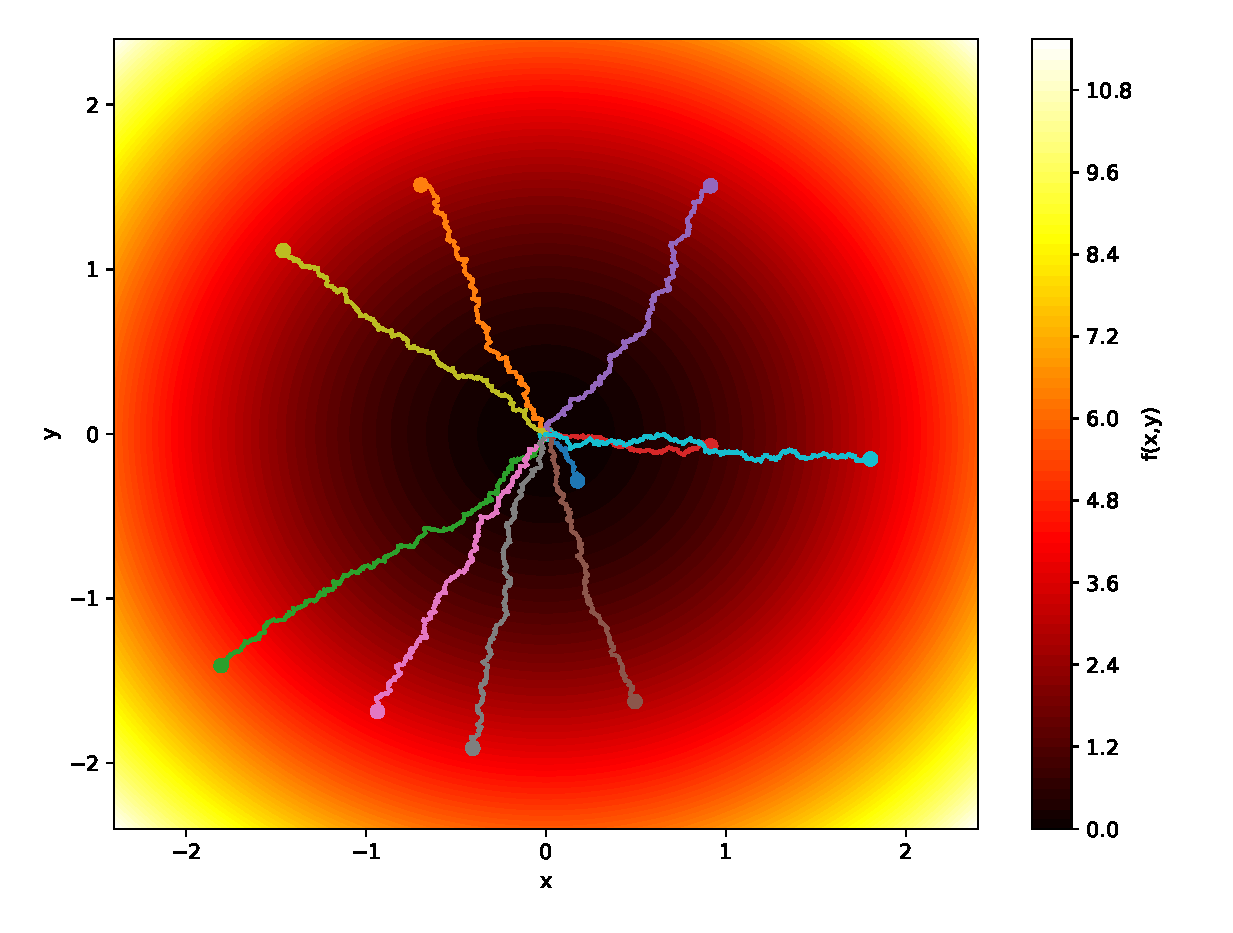
\epsfig{file=quadratic_minimum.eps,width=\linewidth}
            \caption{\code{MultiplePaths(f)}}
        \end{subfigure}
        \hfill
        \begin{subfigure}{0.49\linewidth}
            \centering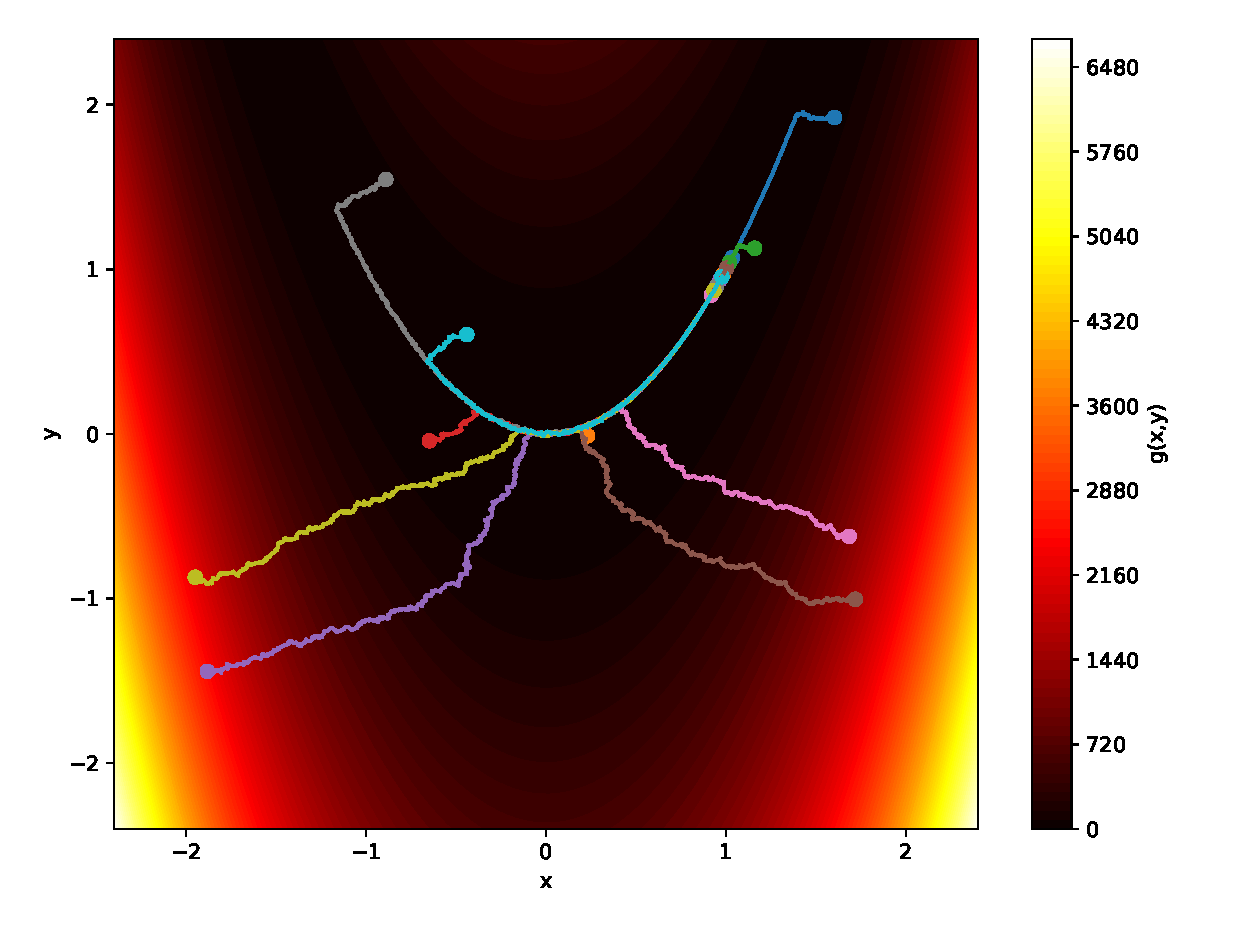
\epsfig{file=rosenbrock_minimum.eps,width=\linewidth}
            \caption{\code{MultiplePaths(g)}}
        \end{subfigure}
        \begin{subfigure}{0.49\linewidth}
            \centering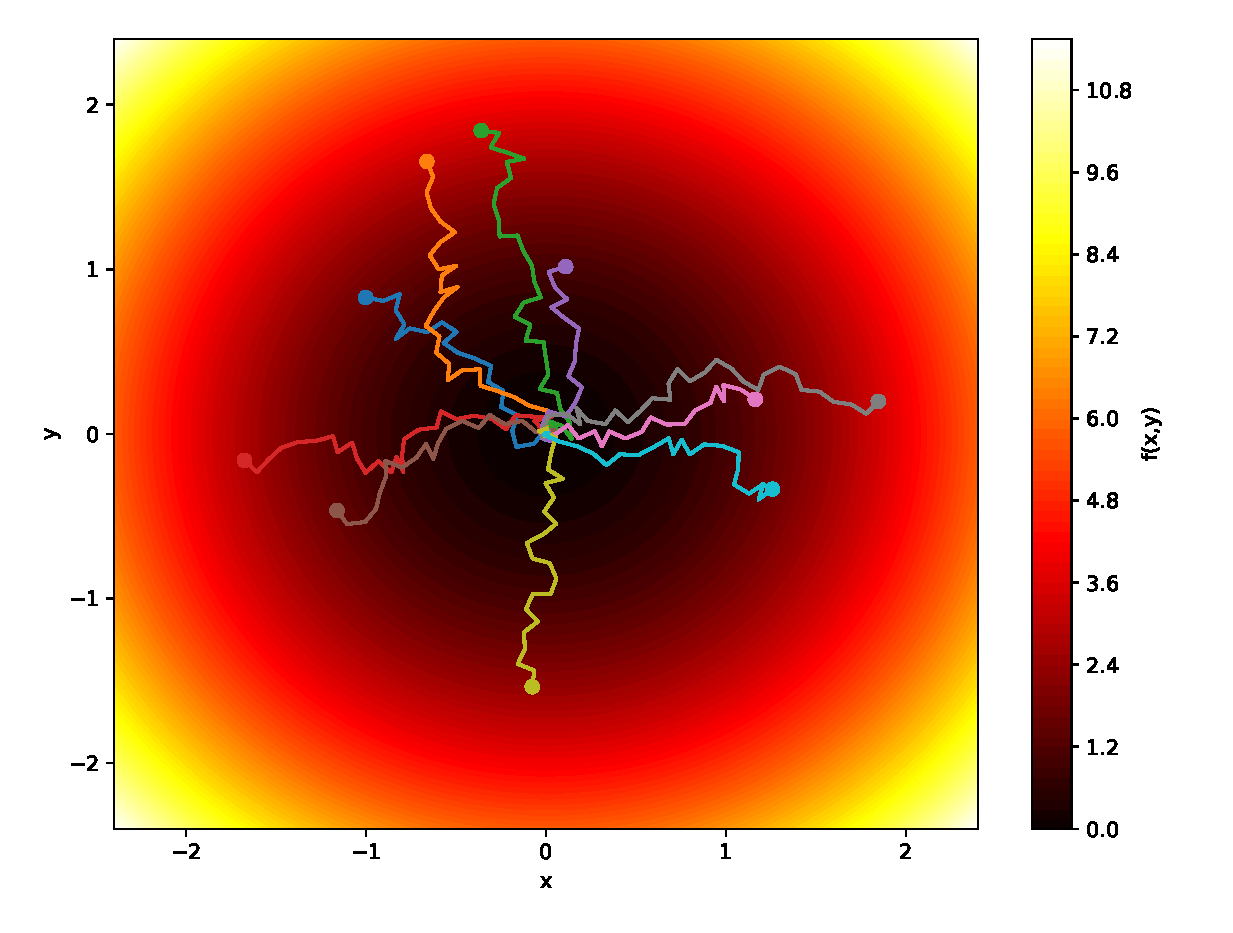
\epsfig{file=quadratic_minimum_adaptive,width=\linewidth}
            \caption{\code{MultiplePathsAdaptive(f)}}
        \end{subfigure}
        \hfill
        \begin{subfigure}{0.49\linewidth}
            \centering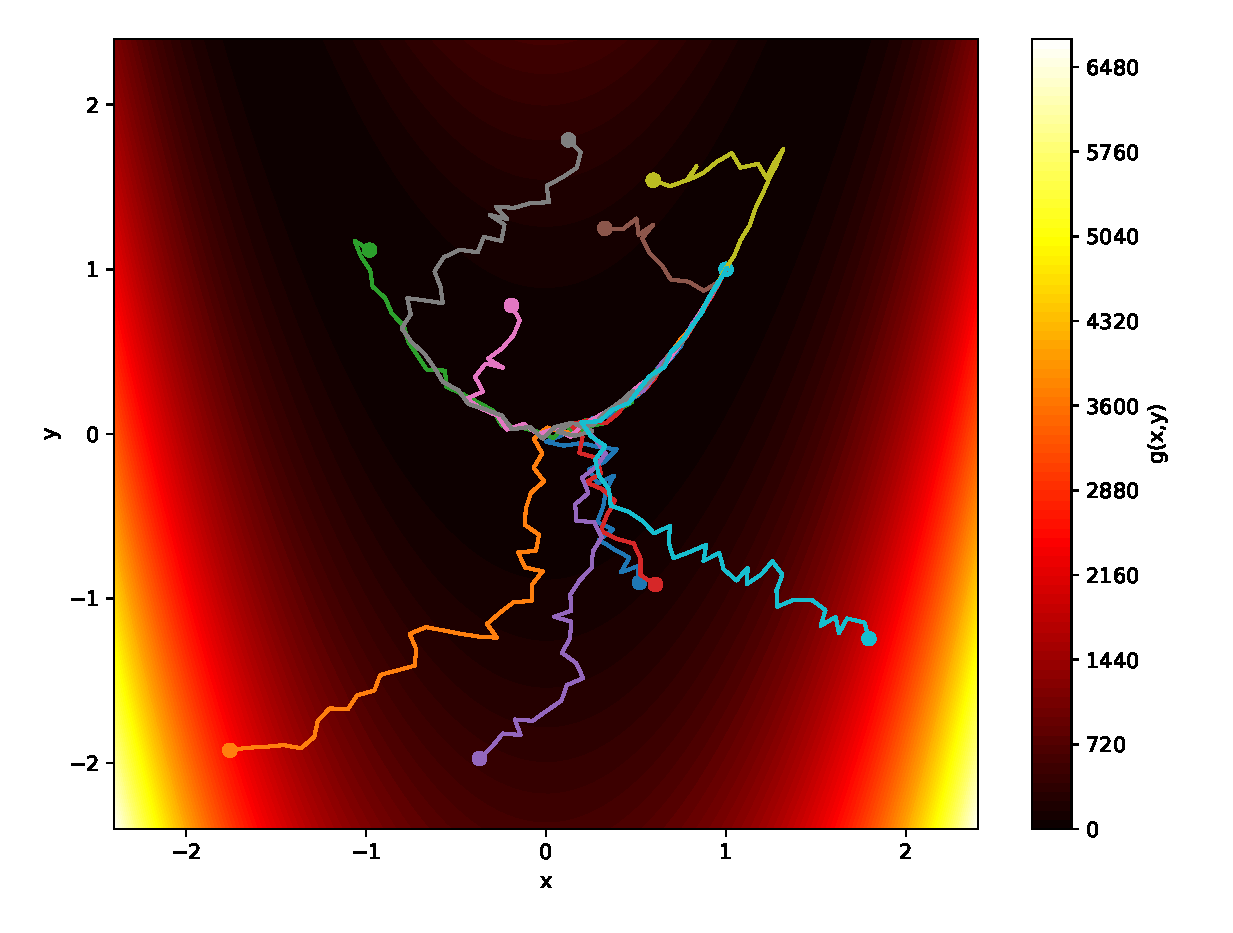
\epsfig{file=rosenbrock_minimum_adaptive.eps,width=\linewidth}
            \caption{\code{MultiplePathsAdaptive(g)}}
        \end{subfigure}

        \caption{
            \protect\small
            Minimalizace kvadratické funkce~\eqref{eq:Minimumf} a Rosenbrockovy funkce~\eqref{eq:Minimumg} pomocí náhodné procházky a deseti trajektorií náhodně vybraných ze čtverce \code{initial_box_size}$\ =2$.
            \emph{1.~řádek:} Minimalizace metodou \code{minimize} s délkou kroku \code{step_size}$\ =0.01$ a kritériem ukončení \code{max_failed_steps}$\ =100$.
            Chyba určení minima je $\Delta x,y\approx0.01$. 
            V případě Rosenbrockova minima je chyba velká: Rosenbrockovo \uv{údolí} je velmi pozvolné podél a strmé napříč, což způsobuje, že trajektorie končí v širokém okolí skutečného minima $(x_{\mathrm{min}},y_{\mathrm{min}})=(1,1)$.
            Počet kroků, než je výpočet ukončen, je zde $\approx1000$.
            \emph{2.~řádek:} Minimalizace vylepšeným algoritmem s postupně se zmenšující krokem.
            Na~počátku je krok velký, \code{initial_step_size}$\ =0.1$, ale postupně se zmešuje až k \code{final_step_size}$\ =10^{-6}$.
            To stačí i pro přesné nalezení minima Rosenbrockovy funkce.
            Počet nutných kroků zde je $\approx3000$.
        }	
        \label{fig:Minimalizacefg}
    \end{figure}

    Vzorový kód je v souboru \ghfile{python/minimize/}{min_functions.py} a využívá jako modul \ghfile{python/minimize/}{minimize.py}.
    Obsahuje následující funkce:
    \begin{itemize}
        \item \code{show_graph}: 
            Vykreslí konturový graf funkce \code{function} a do něj zakreslí křivky (náhodné procházky) z parametru \code{paths}.
            Pokud tento parametr není specifikován, vykreslí pouze konturový graf s funkcí.
            Meze funkce pro vykreslení jsou dány parametrem \code{box_size}.

        \item \code{multiple_paths}:
            Vypočítá celkem \code{num_paths} náhodně vybraných jednoduchých minimalizačních procházek a vykreslí je v grafu společně s konturovým grafem minimalizované funkce.
            Parametrem \code{method} lze určit minimalizaci s pevným krokem nebo s adaptivním krokem.
        \item \code{multiple_paths}:
    \end{itemize}

    Výsledky pro funkce $f$ a $g$ ze zadání jsou zobrazeny na obrázku~\ref{fig:Minimalizacefg}.
\end{solution}

\begin{task}
    Použijte kód pro vícerozměrnou náhodnou procházku a najděte pomocí něho minimum funkce čtyř proměnných
    \begin{align}
        h(s,t,u,v)
            &=\frac{1}{4}\left(s^{2}+t^{2}+u^{2}+v^{2}\right)\nonumber\\
            &\quad-\frac{1}{2}\left[\left(s^{2}+t^{2}\right)\left(2-s^{2}-t^{2}-u^{2}-v^{2}\right)+\left(su-tv\right)^{2}\right]\\
            &\quad+\frac{s}{2}\sqrt{2-s^{2}-t^{2}-u^{2}-v^{2}}\nonumber.
        \end{align}
\end{task}

\begin{solution}
    Volání funkce \code{minimize.minimize_adaptive(h, dimension=4)} vypočítá minimum v bodě
    \begin{align}
        s_{\text{min}}&\approx-0.913\nonumber\\
        t_{\text{min}}=u_{\text{min}}=v_{\text{min}}&\approx0.000\\
        h_{\text{min}}\equiv h(s_{\text{min}},t_{\text{min}},u_{\text{min}},v_{\text{min}})&\approx-0.771.\nonumber
    \end{align}
    V případě minimalizace této funkce je nutné ošetřit odmocninu, pod kterou se může během náhodné procházky objevit záporné číslo, což způsobí konec výpočtu s chybou.
    V kódu je to vyřešeno tak, že v případě kroku do této \uv{nedovolené oblasti} vrátí funkce \code{h} hodnotu $\infty$ (v Pythonu \code{float("inf")}), která je větší než všechna možná jiná čísla, a tím tento krok zakáže.
    Důležitá podmínka však je, že počáteční bod náhodné procházky musí ležet v definičním oboru funkce $h$.
\end{solution}

\begin{task}
    Naprogramujte Metropolisův algoritmus a odlaďte ho na případu funkce
    \begin{equation}\label{eq:Minimumr}
        r(x,y)=x^{4}-2x^{2}+x+y^{2}.
    \end{equation}
    Tato funkce má dvě lokální minima (jedná se o vzorovou funkci ze souboru \ghfile{python/basics/}{contourf.py}).
\end{task}

\begin{solution}
    Pro ukázku, že standardní minimalizace pomocí náhodné procházky vede náhodně do~různých lokálních minim, slouží obrázek~\ref{fig:MetropolisMinimalizacea}.

    \begin{figure}[!htb]
        \centering
        \begin{subfigure}{0.49\linewidth}
            \centering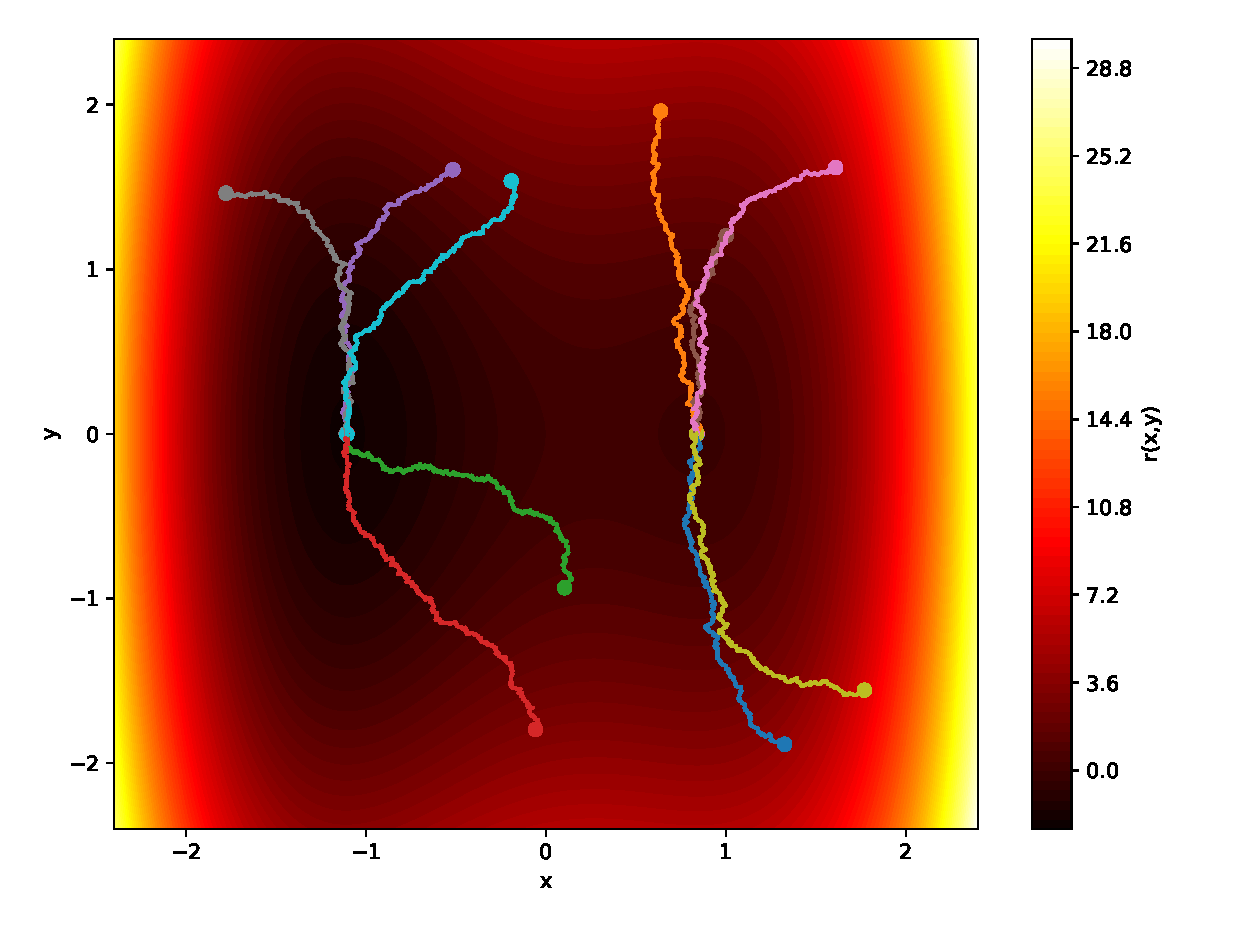
\epsfig{file=double_well_minimum.eps,width=\linewidth}
            \caption{\centering\code{multiple_paths(r, method=minimize.minimize)}}
            \label{fig:MetropolisMinimalizacea}
        \end{subfigure}
        \hfill
        \begin{subfigure}{0.49\linewidth}
            \centering\epsfig{file=double_well_minimum_metropolis.eps,width=\linewidth}
            \caption{\centering\code{multiple_paths(r, method=metropolis.minimize)}}
            \label{fig:MetropolisMinimalizaceb}
        \end{subfigure}
        \hfill
        \begin{subfigure}{0.5\linewidth}
            \centering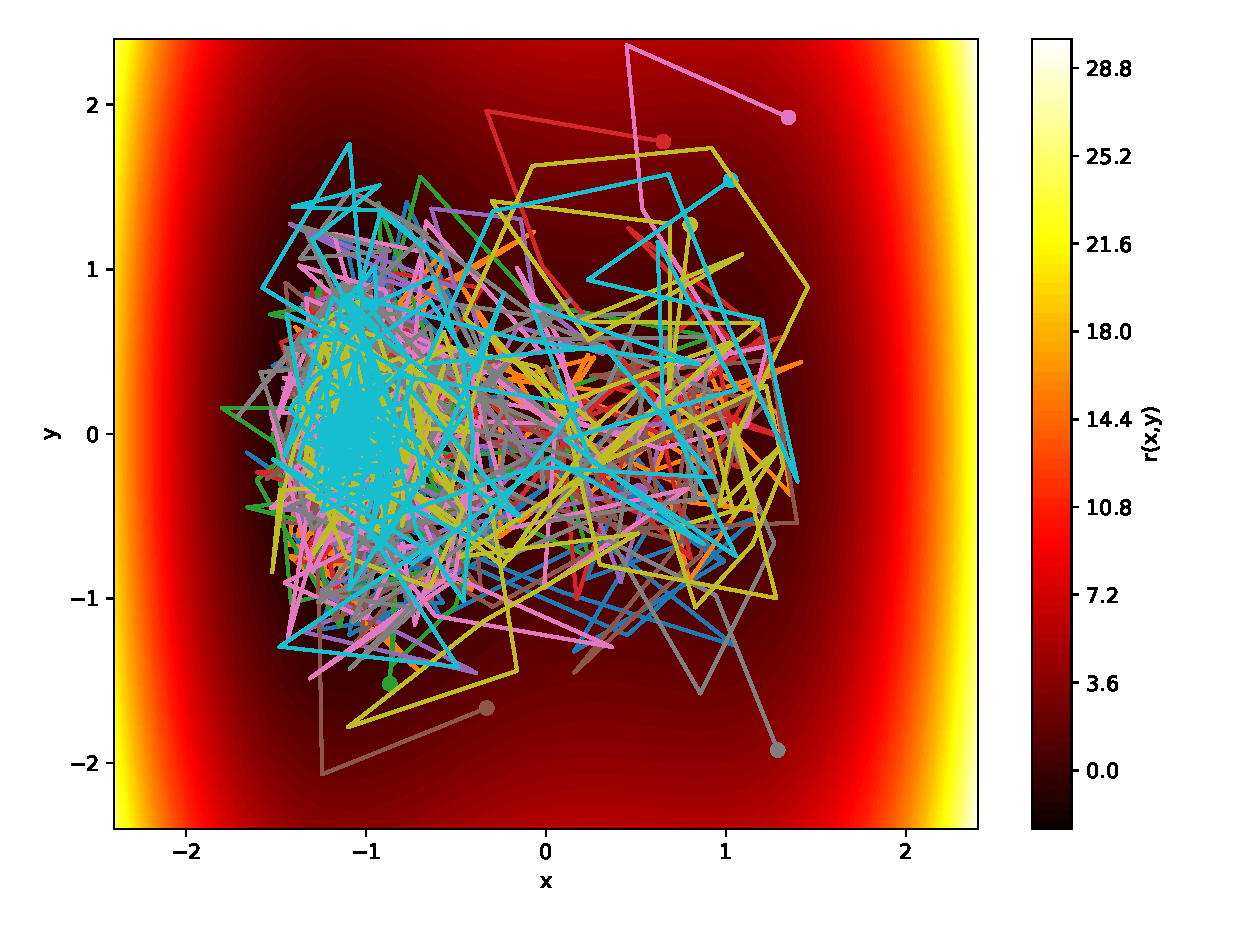
\epsfig{file=double_well_minimum_metropolis_adaptive,width=\linewidth}
            \caption{\centering\code{multiple_paths(r, method=metropolis.minimize_adaptive)}}
            \label{fig:MetropolisMinimalizacec}
        \end{subfigure}
        \hfill

        \caption{
            \protect\small
            Porovnání různých metod minimalizace dvoujámové funkce~\eqref{eq:Minimumr}.
            \subref{fig:MetropolisMinimalizacea} Minimalizace obyčejnou náhodnou procházkou, která dokonverguje do náhodného lokálního minima.
            Následně je možné vybrat to minimum, které je hlubší.
            \subref{fig:MetropolisMinimalizaceb} Metropolisův algoritmus s konstantní teplotou $T=1$.
            Kvůli vysoké teplotě dráha výrazně fluktuuje, avšak postupně dokonverguje k okolí hlubšího globálního minima.
            \subref{fig:MetropolisMinimalizacec} Metropolisův algoritmus s postupně se zmenšujícím krokem a teplotou.
            Zde do globálního minima postupně zkonvergují všechny trajektorie.
            Počet použitých kroků je $2000$.
        }	
        \label{fig:MetropolisMinimalizace}
    \end{figure}
    
    Metropolisův algoritmus je naprogramován v souboru \ghfile{python/randomwalk/}{metropolis.py}.
    \begin{itemize}
        \item \code{minimize}: 
            Minimalizuje funkci \code{function} se zadanou teplotou \code{temperature} a s fixní délkou kroku \code{step_size}. 
            Výpočet je ukončen přesně po \code{max_steps} krocích.
            Kritérium ukončení výpočtu z metody bez teploty zde nebude fungovat, jelikož konečná teplota způsobuje neustálý \uv{tepelný pohyb}, nikdy tedy nedojde k úplnému zastavení, ani pokud dosáhneme minima funkce.

            Výsledek je zobrazen na obrázku~\ref{fig:MetropolisMinimalizaceb}.
            Je vidět, že oproti případu bez teploty se dostaneme častěji k okolí globálního minima, avšak důsledkem celkem vysoké teploty nalezená poloha výrazně fluktuuje.
            Navíc, a to zde není zobrazeno, výsledek velmi silně závisí na kombinaci teploty a délky kroku.
            
        \item \code{minimize_adaptive}:
            Vylepšení spočívající v postupném zmenšování teploty a zároveň kroku.
            Výpočet začne s krokem \code{initial_step_size} a teplotou \code{initial_temperature} a po každých \code{num_steps_change} krocích déku kroku i teplotu vydělí dvěma.
            Výpočet je ukončen po dosažení délky kroku \code{final_step_size}.
            Příklad realizovaných procházek pro funkci~\eqref{eq:Minimumr} je na obrázku~\ref{fig:MetropolisMinimalizacec}.

    \end{itemize}
\end{solution}

\begin{task}
    Prostudujte \href{https://docs.scipy.org/doc/scipy/reference/generated/scipy.optimize.minimize.html}{dokumentaci} k funkci \code{minimize} a vytvořte kód, který tuto funkci využije k najití minima všech doposud studovaných funkcí dvou a více proměnných.
    Pokud programujete v jiném programovacím jazyku, nalezněte odpovídající minimalizační funkci či knihovnu a použijte ji.
\end{task}

\begin{solution}
    Knihovní funkci voláme příkazem \code{minimize(f, initialCondition)}, kde parametr \code{initialCondition} je $n$-tice udávající počáteční bod, ze kterého minimalizační procedura vystartuje.

    V případě funkce s více lokálními minimy tato knihovní funkce nenajde nutně minimum globální.
    Lze však pomocí volitelného parametru \code{method} vybrat metodu minimalizace, která bude úspěšnější.
    Pokročilá varianta Metropolisova algoritmu je v knihovně \file{scipy.optimize} naprogramována pod názvem \code{\href{https://docs.scipy.org/doc/scipy/reference/generated/scipy.optimize.basinhopping.html}{basinhopping}}.
\end{solution}


\subsection{Shrnutí}
    \begin{itemize}
        \item 
            Jeden z nejjednodušších algoritmů na hledání minima (maxima) funkce je pomocí náhodné procházky.
            K její implementaci stačí mít generátor náhodných čísel.

        \item 
            Úspěch algoritmů založených na náhodné procházce je podmíněn tím, že každý krok procházky musí vést do libovolného směru se stejnou pravděpodobností.
            Při procházce v rovině toho lze docílit náhodným generováním úhlu.
            Ve vícerozměrné procházce je nejvýhodnější použít algoritmus založený na Gaussovském náhodném vektoru (za předpokladu, že umíme generovat čísla z Gaussovského rozdělení; jeden jednoduchý takový generátor bude obsahem dalších cvičení).   
        
        \item 
            Obecná funkce může mít více lokálních minim, přičemž náhodná procházka nás zavede do jednoho z nich, které nemusí být nejhlubší (globální).
            K nalezení globálního minima lze využít Metropolisův algoritmus, který k náhodné procházce přidá tepelný pohyb, a tím umožní \uv{vyskočit} z mělkého lokálního minima.  

            Metropolisův algoritmus se využívá i pro jiné termodynamické úlohy, například k modelování spinových systémů při konečné teplotě, čímž lze studovat fázový přechod feromagnet $\leftrightarrow$ paramagnet.
    \end{itemize}


\section{Histogram}
    V tomto cvičení budeme pokračovat s náhodnými čísly, se kterými již pracovali při programování náhodné procházky v \ref{sec:NahodnaProchazka}. sekci.
    Zde se podíváme hlouběji na jejich vlastnosti, naučíme se zobrazit hustotu pravděpodobnosti jejich rozdělení (histogram), vytvoříme triviální generátor čísel z Gaussovského normálního rozdělení a generátor čísel z libovolného rozdělení zadaného hustotou pravděpodobnosti nebo distribuční funkcí.
       
    Histogram je jeden z klíčových objektů v mnoha oblastech fyziky, kde se pracuje s náhodnými veličinami.
    To je vpodstatě celá kvantová mechanika, a tudíž obory jako je atomová, jaderná, či subjaderná fyzika.
    S náhodnými veličinami se setkáte samozřejmě také v klasické statistické fyzice, ale také například v meteorologii či dalších oborech.
    Stojí proto za to se s histogramem seznámit podrobně.

    \subsection{Základní definice a tvrzení z teorie pravděpodobnosti}
    \label{sec:Pravdepodobnost}
        V následujícím textu budeme značit $X$ spojitou náhodnou veličinu\footnote{
            V teorii pravděpodobnosti se náhodné veličiny značí obvykle velkým písmenem.
        } s hodnotami v intervalu $x\in\langle a,b\rangle$\footnote{
            Náhodná veličina $X$ je ve skutečnosti velmi abstraktní objekt.
            Obecně se definuje na měřitelném prostoru $(\mathcal{X},\mathcal{A},\mu)$, kde $\mathcal{X}$ je množina možných hodnot náhodné veličiny $X$, $\mathcal{A}$ je $\sigma$-algebra nad množinou $\mathcal{X}$ (neprázdný systém množin uzavřený na spočetné sjednocení a obsahující prázdnou množinu a množinu $\mathcal{X}$) a $\mu$ je míra množiny $\mathcal{M}\subset\mathcal{X}$ (nezáporná $\sigma$-aditivní množinová funkce nulová pro prázdnou množinu a jednotková pro celou množinu $\mathcal{X}$).
            Tato definice v sobě zahrnuje jak náhodné veličiny s diskrétními možnými hodnotami (jako je například hod kostkou), tak náhodné veličiny se spojitými možnými hodnotami, kterým se věnujeme v této sekci.
        }.
        Důležité pojmy a vztahy pro nás budou:
        \begin{itemize}
            \item {\bf Hustota pravděpodobnosti  $\rho(x)$:}
                Pravděpodobnost, že náhodná veličina $X$ bude nabývat hodnoty z intervalu $\left\langle x_{1},x_{2}\right\rangle\subset\langle a,b\rangle$, je
                \begin{equation}
                    \probability{x_{1}\le X\le x_{2}}=\int_{x_{1}}^{x_{2}}\rho(x)\d x.
                \end{equation}
                Hustota pravděpodobnosti je normalizovaná na definičním oboru,
                \begin{equation}\label{eq:rhoNorm}
                    \int_{a}^{b}\rho(x)\d x=1
                \end{equation}
                (pravděpodobnost, že bude náhodná veličina nabývat libovolné ze svých povolených hodnot, je $1=$ jistý jev).
                Hustotu pravděpodobnosti lze vždy rozšířit na celou množinu $\mathbb{R}$, pokud dodefinujeme $\rho(x)=0$ pro $x<a$ a $x>b$.

            \item {\bf Distribuční funkce (kumulovaná hustota pravděpodobnosti) $F(x)$:} 
                Neklesající spojitá funkce s oborem hodnot $\langle 0,1\rangle$ daná integrálem hustoty pravděpodobnosti\footnote{
                    Nebo obráceně, hustota pravděpodobnosti je derivace distribuční funkce,
                    \begin{equation}
                        \label{eq:rhoF}
                        \rho(x)=\derivative{F}{x}.
                    \end{equation}
                }
                \begin{equation}
                    F(x)=\int_{a}^{x}\rho(x')\d x'.
                \end{equation}
                Platí tedy díky normalizaci~\eqref{eq:rhoNorm}
                \begin{align*}
                    F(a)&=0,\\
                    F(b)&=1.
                \end{align*}
                Rozšíříme-li obor hodnot náhodné veličiny na všechna reálná čísla stejným způsobem, jako jsme naznačili u hustoty pravděpodobnosti, platí navíc
                \begin{align*}
                    F(x<a)&=0,\\
                    F(x>b)&=1.
                \end{align*}
                Pravděpodobnost, že náhodná veličina $X$ bude nabývat hodnoty z intervalu $\left\langle x_{1},x_{2}\right\rangle$, je pak jednoduše
                \begin{equation}
                    \probability{x_{1}\le X\le x_{2}}=F(x_{2})-F(x_{1}).
                \end{equation}

            \item {\bf Střední hodnota:}\footnote{{\bf E}xpectation value}
                \begin{equation}
                    \label{eq:Expectation}
                    \expectation{X}=\int_{-\infty}^{\infty}x\rho(x)\d x.
                \end{equation}

            \item {\bf Rozptyl:}
                \begin{equation}
                    \label{eq:Dispersion}
                    \dispersion{X}
                        =\expectation{X^{2}}-\expectation{X}^{2}
                        =\int_{-\infty}^{\infty}x^{2}\rho(x)\d x-\left[\int_{\infty}^{\infty}x\rho(x)\d x\right]^{2}.
                \end{equation}

            \item {\bf Výběrová střední hodnota:} 
                Pokud máme soubor $n$ hodnot náhodné veličiny $X$, které označíme $\left\{x_{1},x_{2},\dotsc,x_{n}\right\}$ (výběr), pak výběrová střední hodnota je dána aritmetickým průměrem,
                \begin{equation}
                    \overline{X}=\frac{1}{n}\sum_{j=1}^{n}x_{n}.
                \end{equation}
                Čím mohutnější máme výběr, tím lépe výběrová střední hodnota aproximuje střední hodnotu,
                \begin{equation}
                    \overline{X}\xrightarrow{n\rightarrow\infty}\expectation{X}.
                \end{equation}

            \item {\bf Histogram:}
                Graf (obvykle sloupcový), který aproximuje distribuční funkci náhodné veličiny $X$ na základě hodnot výběru $\mathcal{V}=\{x_{j},j=1,\dotsc,n\}$.
                Graf se skládá z $N\ll n$ intervalů (sloupců) obvykle konstantní šířky pokrývající obor hodnot náhodné veličiny $\langle a,b\rangle$, přičemž výška sloupce na konkrétním intervalu je rovna počtu hodnot z výběru $\mathcal{V}$, které do intervalu padnou.
                Pokud histogram správně nanormujeme, získáme (poněkud zubatou) aproximaci distribuční funkce.

            \item{\bf Nezávislé náhodné veličiny:}
                Dvě náhodné veličiny $X$ a $Y$ jsou nezávislé, pokud jedna neovlivňuje druhou.
                Sdružená hustota pravděpodobnosti nezávislých náhodných veličin je dána součinem dílčích hustot pravděpodobnosti,
                \begin{equation}
                    \rho_{X,Y}(x,y)=\rho(x)\rho(y).
                \end{equation}
                Například věk a výška náhodně vybrané osoby nejsou nezávislé veličiny (pro děti bude rozdělení jejich výšek jiné než pro dospělé), zatímco věk osoby a její krevní skupina nezávislé veličiny jsou.

            \item {\bf Součet dvou náhodných veličin:} 
                Pokud máme náhodnou veličinu $X$ s hustotou pravděpodobnosti $\rho_{X}(x)$ a náhodnou veličinu $Y$ s hustotou pravděpodobnosti $\rho_{Y}(y)$, přičemž obě náhodné veličiny jsou nezávislé, pak náhodná veličina
                \begin{equation}
                    Z=X+Y
                \end{equation}
                bude mít hustotu pravděpodobnosti $\rho_{Z}$ danou \emph{konvolucí} hustot $\rho_{X}$ a $\rho_{Y}$,
                \begin{equation}
                    \label{eq:SumDensity}
                    \rho_{Z}(z)=\int_{-\infty}^{\infty}\rho_{X}(\xi)\rho_{Y}(z-\xi)\d\xi.
                \end{equation}
                Střední hodnota a rozptyl náhodné veličny $Z$ jsou dány součtem 
                \begin{align}
                    \expectation{Z}&=\expectation{X}+\expectation{Y},\nonumber\\
                    \dispersion{Z}&=\dispersion{X}+\dispersion{Y}.
                \end{align}

            \item {\bf Centrální limitní věta:}
                Je-li náhodná veličina $Y$ daná součtem $m$ vzájemně nezávislých náhodných veličin $X^{(1)},X^{(2)},\dotsc,X^{(m)}$ se shodným rozdělením s hustotou pravděpodobnosti $\rho(x)=\rho_{X^{(j)}}(x)$, jehož střední hodnota je $\mu\equiv\expectation{X^{(j)}}<\infty$ a $\sigma^{2}\equiv\dispersion{X^{(j)}}<\infty$, $j=1,\dotsc,m$,
                pak 
                \begin{equation}
                    \label{eq:CLT}
                    Y\sim N(m\mu,m\sigma^{2}),
                \end{equation}
                kde $N(\mu,\sigma^{2})$ je Gausovské normální rozdělení se střední hodnotu $\mu$ a rozptylem $\sigma^{2}$.
                Zcela ekvivalentně lze zavést náhodnou veličinu $U$ jako přeškálovanou veličinu $Y$ a psát
                \begin{equation}
                    \label{eq:CLT1}
                    U\equiv\frac{Y-m\mu}{\sqrt{m\sigma^{2}}}\xrightarrow{n\rightarrow\infty}N(0,1).
                \end{equation}
                Hustota pravděpodobnosti normálního rozdělení je dána vzorcem~\eqref{eq:NormalDistribution}.
        \end{itemize}

    \subsection{Příklady náhodných veličin}
        \begin{itemize}
            \item {\bf Rovnoměrné rozdělení $R(a,b)$ na intervalu $\langle a,b\rangle$:}
                \begin{align}
                    \label{eq:UniformDistribution}
                    \rho_{R}(x)&=\frac{1}{b-a}=\text{konst.}\\
                    \label{eq:ExpectationR}
                    \expectation{R}&=\frac{a+b}{2}\\
                    \label{eq:DispersionR}
                    \dispersion{R}&=\frac{(b-a)^{2}}{12}.
                \end{align} 

            \item {\bf Gaussovo normální rozdělení $N\left(\mu,\sigma^{2}\right)$:}
                \begin{align}
                    \label{eq:NormalDistribution}
                    \rho_{N}(x)&=\frac{1}{\sqrt{2\pi\sigma^{2}}}\e^{-\frac{(x-\mu)^{2}}{2\sigma^{2}}}\\
                    \expectation{N}&=\mu\\
                    \dispersion{N}&=\sigma^{2}.
                \end{align} 

            \item {\bf Poissonovo rozdělení:}
                Diskrétní rozdělení udávající počet nezávislých jevů $k$ v zadaném intervalu (například počet lidí, které potkáte na mostě cestou z Holešovic do Troji, počet kapek, které vám za nějakou časovou jednotku spadne na hlavu, počet rozpadů radioaktivního prvku ve vzorku za jednotku času atd.).  
                Rozdělení pravděpodobnosti je
                \begin{align}
                    \label{eq:Poisson}
                    P_{k}&=\frac{\lambda^{k}}{k!}\e^{-\lambda},\\
                    \label{eq:ExpectationP}
                    \expectation{P}&=\lambda,\\
                    \label{eq:DispersionP}
                    \dispersion{P}&=\lambda,
                \end{align}
                přičemž parametr $\lambda$ udává zároveň střední hodnotu a zároveň rozptyl rozdělení.
        \end{itemize}

    \begin{voluntary}
        Dokažte vztahy~\eqref{eq:ExpectationR}--\eqref{eq:DispersionR} a \eqref{eq:ExpectationP}--\eqref{eq:DispersionR}.
    \end{voluntary}

    \begin{solution}
        K dokázání~\eqref{eq:ExpectationR}--\eqref{eq:DispersionR} vyjdeme z definičních vztahů pro střední hodnotu a rozptyl~\eqref{eq:Expectation}--\eqref{eq:Dispersion}:
        \begin{align}
            \expectation{R}
                &=\int_{a}^{b}\frac{x}{b-a}\d x
                =\frac{1}{b-a}\left[\frac{x^{2}}{2}\right]_{a}^{b}
                =\frac{1}{b-a}\frac{b^{2}-a^{2}}{2}
                =\frac{a+b}{2},\\
            \dispersion{R}
                &=\int_{a}^{b}\frac{x^{2}}{b-a}\d x-\left(\frac{a+b}{2}\right)^{2}
                =\frac{1}{b-a}\frac{b^{3}-a^{3}}{3}-\frac{(a+b)^{2}}{4}\nonumber\\
                &=\frac{a^{2}+ab+b^{2}}{3}-\frac{a^{2}+2ab+b^{2}}{4}
                =\frac{a^{2}-2ab+b^{2}}{12}=\frac{(b-a)^{2}}{12}.
        \end{align}

        Poissonovo rozdělení je diskrétní, je tudíž nutné použít diskrétní analogii vztahů~\eqref{eq:Expectation}--\eqref{eq:Dispersion} (nahrazení integrálů sumami):
        \begin{align}
            \expectation{P}
                &=\sum_{k=0}^{\infty}kP_{k}
                =\sum_{k=1}^{\infty}\frac{\lambda^{k}}{(k-1)!}\e^{-\lambda}
                =\left|\begin{array}{c}\text{substituce} \\ l=k-1\end{array}\right|
                =\sum_{l=0}^{\infty}\frac{\lambda^{l+1}}{l!}\e^{-\lambda}=\lambda,\\
            \dispersion{P}
                &=\sum_{k=0}^{\infty}k^{2}P_{k}-\lambda^{2}
                =\sum_{k=1}^{\infty}\frac{k\lambda^{k}}{(k-1)!}\e^{-\lambda}-\lambda^{2}\nonumber\\
                &=\sum_{k=1}^{\infty}\frac{(k-1)\lambda^{k}}{(k-1)!}\e^{-\lambda}+\sum_{k=1}^{\infty}\frac{\lambda^{k}}{(k-1)!}\e^{-\lambda}-\lambda^{2}\nonumber\\
                &=\sum_{k=2}\frac{\lambda^{k}}{(k-2)!}\e^{-\lambda}+\lambda-\lambda^{2}
                =\lambda^{2}+\lambda-\lambda^{2}=\lambda.
        \end{align}
    \end{solution}

    \subsection{Výběr z neznámého rozdělení}\label{sec:SelectDistribution}
        V praxi se můžeme setkat se situací, kdy máme zadanou hustotu pravděpodobnosti či distribuční funkci nějakého komplikovaného rozdělení a chceme generovat výběr z tohoto rozdělení.

        \begin{itemize}
            \item {\bf Známe-li hustotu pravděpodobnosti rozdělení $\rho(x)$:}
                Nejjednodušší metoda v tomto případě je vepsat funkci $\rho(x)$ do obdélníku $\langle a,b\rangle\times\langle c,d\rangle$\footnote{
                    Hustota pravděpodobnosti bývá obvykle definovaná na neomezeném intervalu.
                    Pak je nutné určitou část funkce $\rho(x)$ oříznout.
                    To funguje dobře v případě náhodných veličin s rychle ubývající hustotou pravděpodobnosti, jako je například Gaussovo rozdělení $N(0,1)$, kde při oříznutí $x\in\langle-3\sigma,3\sigma\rangle=\langle-3,3\rangle$ zanedbáme jen 3\textperthousand{} možných hodnot.
                    V~případě dlouhodosahových rozdělení, jako je například lognormální rozdělení nebo Gamma rozdělení, musíme obdélník volit velmi dlouhý, čímž se tato metoda stává velmi neefektivní.
                }, nagenerovat číslo rovnoměrně z tohoto obdélníku, a pokud padne pod křivku $\rho(x)$, vezmeme ho, v opačném případě ho zahodíme (tzv. \emph{hit-and-miss metoda}, se kterou se ještě potkáme u metody Monte-Carlo).

            \item {\bf Známe-li distribuční funkcí $F(x)$:}
                V tomto případě využijeme skutečnosti, že obor hodnot distribuční funkce je $F(x)\in\langle0,1\rangle$. 
                Stačí tedy generovat náhodné číslo $y$ z rovnoměrného rozdělení na intervalu $\langle0,1\rangle$ a číslo 
                \begin{equation}
                    \label{eq:xF}
                    x=F^{-1}(y),
                \end{equation}
                kde $F^{-1}$ je inverzní funkce k $F$, bude z rozdělení s danou $F$.
                Pokud neznáme inverzní funkci, řešíme numericky rovnici
                \begin{equation}
                    F(x)=y,
                \end{equation}
                která však s ohledem na vlastnosti distribuční funkce popsané v sekci~\ref{sec:Pravdepodobnost} má téměř vždycky jedno a pouze jedno řešení.

                Matematičtěji zapsáno: je-li $R=R(0,1)$ náhodná veličina s rovnoměrným rodělením na intervalu $\langle0,1\rangle$, pak
                \begin{equation}
                    X=F^{-1}(R)
                \end{equation}
                je náhodná veličina s rozdělením daným distribuční funkcí $F$.
        \end{itemize}

\newpage
{\color{red}\subsection{Domácí úkol na 20.4.2021}}
    \begin{task}
        Naprogramujte funkci pro výpočet histogramu: na vstupu bude pole hodnot (výběr z nějakého rozdělení) a počet intervalů histogramu; na výstupu bude pole, jehož každý prvek bude odpovídat jednomu intervalu histogramu a ponese počet hodnot, které do tohoto intervalu padnou ze vstupního pole.
        Nejefektivnějšímu algoritmu stačí jeden průchod vstupním polem (jeden cyklus). 
        Pokuste se na něj přijít.

        Výstupní pole funkce vykreslete jako čárový graf.\footnote{
            Knihovna \code{matplotlib} obsahuje funkce na přímé vykreslení sloupcového histogramu, například \code{\href{https://matplotlib.org/stable/api/_as_gen/matplotlib.pyplot.hist.html}{hist}}.
        }
    \end{task}

    \begin{solution}
        Vzorový výpočet histogramu je naprogramován v souboru \ghfile{python/histogram/}{histogram.py} ve funkci \code{histogram}.
        Klíčové jsou dva řádky:

        \begin{lstlisting}[style=NormalPython]
    index = int((d - min_value) / bin_width
    histogram[index] += 1\end{lstlisting}
        Hodnota, kterou chceme zařadit do příslušného okénka histogramu, se nachází v proměnné \code{d}.
        Z ní spočítáme celočíselný index v intervalu mezi $0\leq\mathtt{index}<\mathtt{num_bins}$ a pak v poli histogram na příslušném indexu přidáme jedničku.
        Histogramované pole hodnot \code{data} tedy stačí procházet jen jednou, algoritmus má tudíž časovou náročnost $\mathcal{O}(N)$.
        Nutným předpokladem pro použití tohoto algoritmu je, že všechna okénka histogramu musejí mít stejnou šířku.
        Funkce \code{histogram} pak vrací pole s $x$-ovými hodnotami (středy histogramů) a pole s hotovým histogramem.
        Pro snazší porovnání s hustotami pravděpodobnosti lze navíc nastavit parametr \code{normalize=True}, výsledný histogram pak bude splňovat
        \begin{equation}
            \sum_{i=1}^{\mathtt{num\_bins}}h_{i}w_{i}=1,
        \end{equation}
        kde $h_{i}$ je hodnota histogramu v $i$-tém okénku a $w_{i}\equiv\mathtt{bin\_width}$ šířka okénka.

        \begin{figure}[!htbp]
            \begin{subfigure}{0.49\linewidth}
                \centering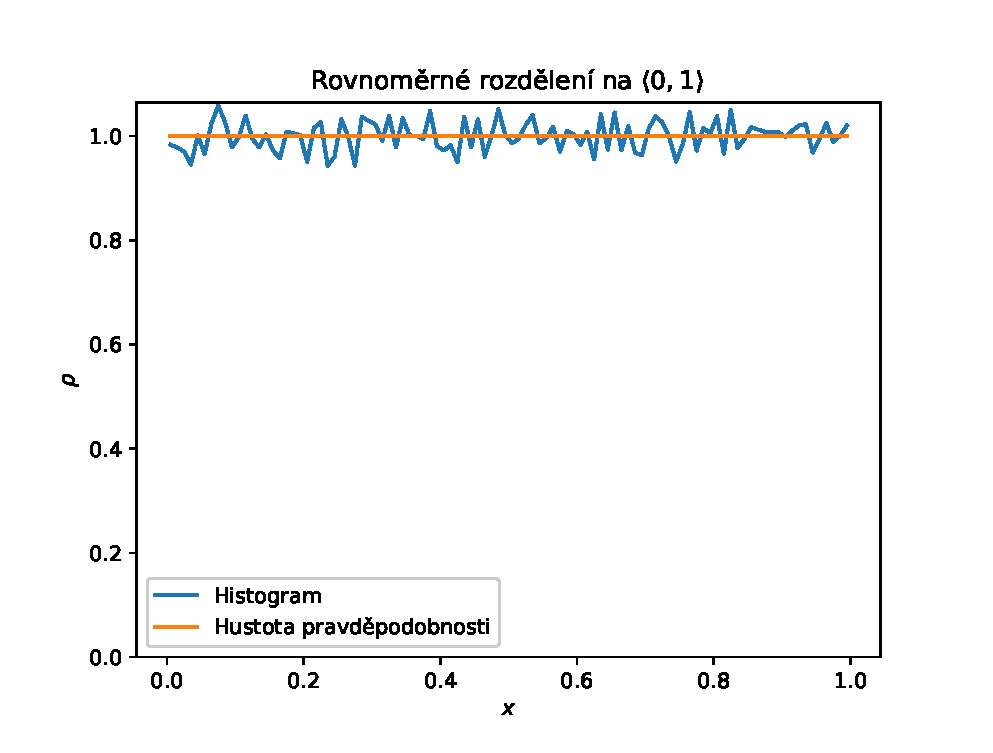
\epsfig{file=uniform.eps,width=\linewidth}
                \caption{}
            \end{subfigure}
            \hfill
            \begin{subfigure}{0.49\linewidth}
                \centering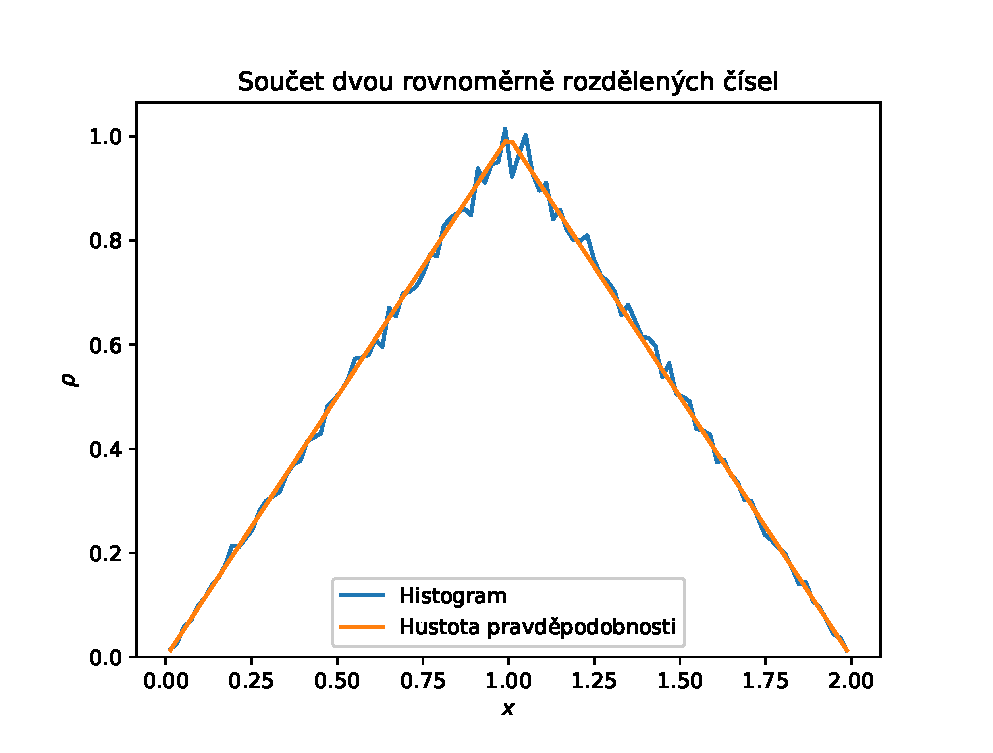
\epsfig{file=uniform2.eps,width=\linewidth}
                \caption{}
            \end{subfigure}
            \caption{
                \protect\small
                Srovnání histogramu získaného z $n=10^{5}$ hodnot vybraných z daného rozdělení a porovnání s teoretickou hustotou pravděpodobnosti (a) rovnoměrného rozdělení~\eqref{eq:UniformDistribution} ($a=0,b=1$) a (b) součtu dvou rovnoměrných rozdělení~\eqref{eq:2UniformDistribution}.
                Počet intervalů histogramu je v obou případech $N=100$.
            }
            \label{fig:Distributions}
        \end{figure}
        
        Příklady histogramů a jejich vykreslení do grafu jsou v řešení následujícího úkolu a na obrázku~\ref{fig:Distributions}.
    \end{solution}

    \begin{task}\label{task:Distributions}
        Otestujte funkci z předchozího úkolu na následujících vstupních datech:
        \begin{enumerate}
            \item
                Výběr z rovnoměrného rozdělení na intervalu $\langle 0,1\rangle$ (v Pythonu generované pomocí \code{random()} z knihovny \file{random}, resp. pomocí \code{generator.random()} z knihovny \file{numpy.random}, jak je shrnuto v sekci~\ref{sec:PseudonahodnaCisla}).
            \item
                Výběr ze {\bf součtu dvou} rovnoměrných rozdělení na intervalu $\langle 0,1\rangle$.
                Hustota pravděpodobnosti výsledného rozdělení je dána konvolucí~\eqref{eq:SumDensity}.
                Vypočítejte analyticky pomocí tohoto vzorce, jak bude hustota pravděpodobnosti vypadat, a porovnejte se získaným histogramem.
            \item
                Výběr ze {\bf součtu $m$} rovnoměrných rozdělení na intervalu $\langle 0,1\rangle$.
                Přesvědčte se, že již pro celkem malé $m$ platí centrální limitní věta~\eqref{eq:CLT} a výsledné rozdělení se blíží normálnímu rozdělení $N(\mu,\sigma)$.
                Jaká bude střední hodnota $\mu$ a rozptyl $\sigma$ tohoto rozdělení?
        \end{enumerate}
        Pro pěkné grafy volte alespoň $n=10000$ (počet prvků výběru) a $N=100$ (počet intervalů histogramu).
    \end{task}
    
    \begin{solution}
        Testování funkce \code{histogram} pro různá rozdělení je v souboru \ghfile{python/histogram/}{distributions.py}.
        \begin{enumerate}
            \item 
                Hustota pravděpodobnosti rovnoměrného rozdělení je zobrazena funkcí \code{uniform}.
                Výsledný graf je na obrázku~\ref{fig:Distributions}.

            \item
                Hustota pravděpodobnosti součtu dvou rovnoměrných rozdělení je podle~\eqref{eq:SumDensity}
                \begin{align}
                    \rho_{2}(z)
                        =\int_{0}^{1}\rho_{1}(\xi)\rho_{1}(z-\xi)\d\xi
                        =\int\rho_{1}(z-\xi)\d\xi,
                \end{align}
                kde $\rho_{1}(\xi)=1$ pro $0\leq\xi\leq1$ a $\rho_{1}(\xi)=0$ jinde,
                čímž se v integrálu zbavíme faktoru $\rho_{1}(\xi)$, neboť je rovný $1$ na celém integračním intervalu.
                Integraci nyní rozdělíme na čtyři intervaly:
                \begin{align}
                    z&<0: &
                    \rho_{2}(z)&=0,\nonumber\\
                    0&<z<1: &
                    \rho_{2}(z)&=\int_{0}^{z}\d\xi=z,\nonumber\\
                    1&<z<2: &
                    \rho_{2}(z)&=\int_{z-1}^{z}\d\xi=1-(1-z)=2-z,\nonumber\\
                    z&>2: &
                    \rho_{2}(z)&=0.\nonumber
                \end{align}
                To lze zapsat zjednodušeně jako
                \begin{equation}
                    \label{eq:2UniformDistribution}
                    \rho_{2}(z)=\left\{\begin{array}{ll}
                        1-\abs{1-z} & 0<z<2, \\
                        0 & \text{jinak}.
                    \end{array}\right.
                \end{equation}
                Rozdělení má trojúhelníkový tvar, což odráží skutečnost, že při součtu dvou rovnoměrně rozdělených čísel na intervalu $\langle0,1\rangle$ je mnohem více možností, jak realizovat součet okolo $1$, než součet na krajích intervalu (stejně jako při hodu dvěma kostkami je největší pravděpodobnost součtu rovna $7$, jak vědí všichni hráči deskové hry \href{https://cs.wikipedia.org/wiki/Osadn%C3%ADci_z_Katanu}{Osadníci z Katanu}  a je větší než pravděpodobnost součtu $12$, neboť součet $7$ můžeme realizovat šesti způsoby z $36$ celkových možných výsledků hodu dvěma kostkami, zatímco součet $12$ jen jedním způsobem).
                Hustota pravděpodobnosti se počítá funkcí \code{sum_2_uniform} a výsledný graf je zobrazen na obrázku~\ref{fig:Distributions}.
            
            \item  
                Výpočet hustoty pravděpodobnosti součtu více rovnoměrných rozdělení je naprogramován ve funkci \code{sum_m_uniform} a porovnání se správně nanormovanou Gaussovkou je na obrázku~\ref{fig:Gaussian}. 
        \end{enumerate}

        \begin{figure}[!htb]
            \begin{subfigure}{0.33\linewidth}
                \centering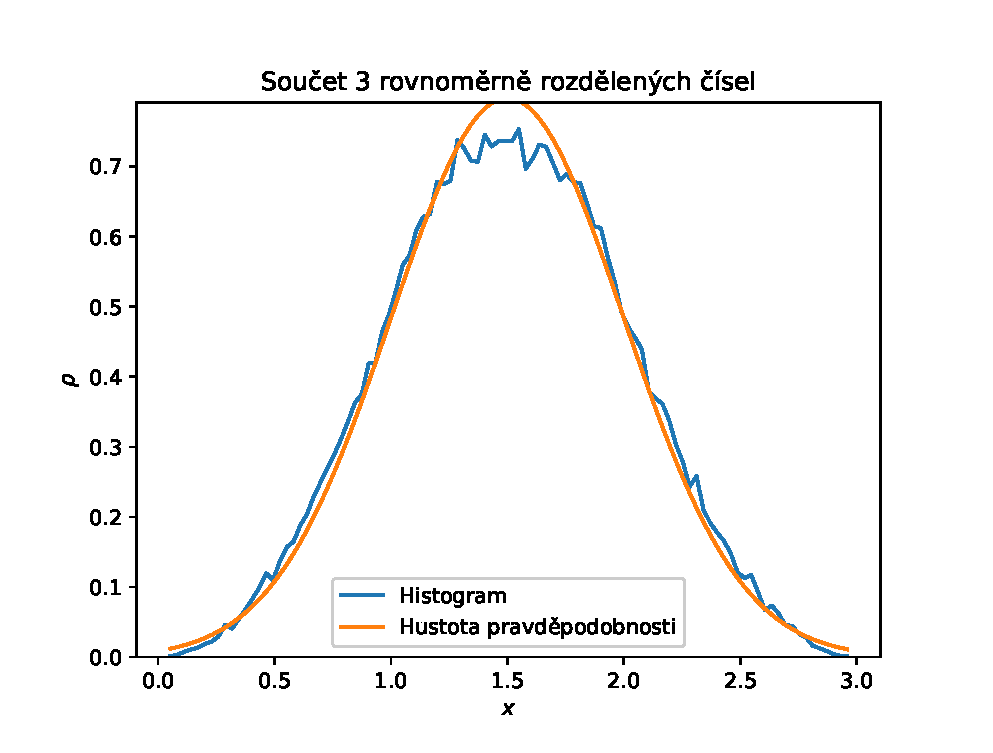
\epsfig{file=uniform3.eps,width=\linewidth}
                \caption{}
            \end{subfigure}
            \begin{subfigure}{0.33\linewidth}
                \centering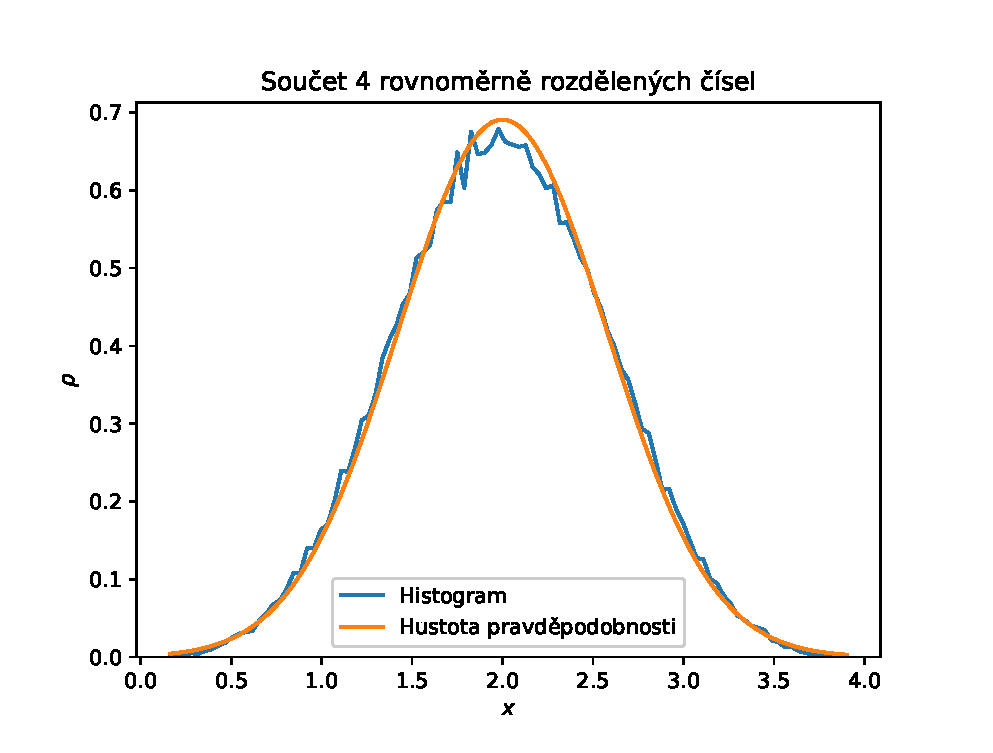
\epsfig{file=uniform4.eps,width=\linewidth}
                \caption{}
            \end{subfigure}
            \begin{subfigure}{0.33\linewidth}
                \centering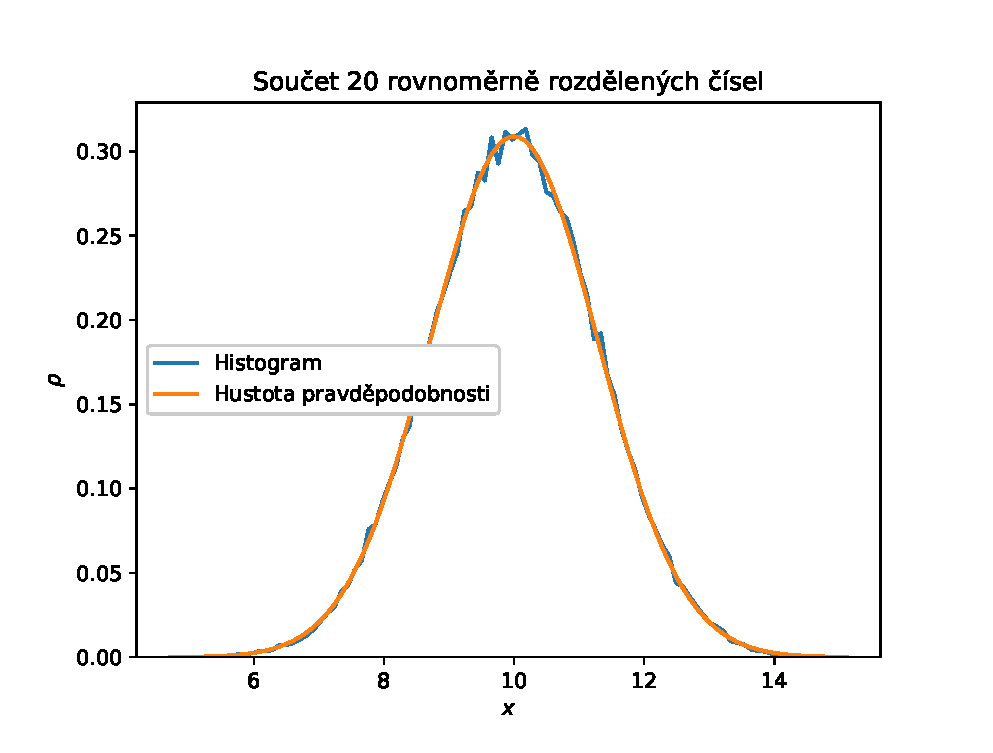
\epsfig{file=uniform20.eps,width=\linewidth}
                \caption{}
            \end{subfigure}
            \caption{
                \protect\small
                Srovnání histogramu získaného z $n=10^{5}$ hodnot daných součtem (a) $m=3$, (b) $m=4$ a (c) $m=20$ rovnoměrně rozdělených náhodných čísel, s Gaussovskou hustotou pravděpodobnosti. 
                Již pro $m=3$ je shoda velmi dobrá a centrální limitní věta~\eqref{eq:CLT} je přibližně splněna.
                V případě $m=20$ je již rozdíl od Gaussovského rozdělení prakticky nepozorovatelný.
                Počet intervalů histogramu je ve všech případech $N=100$.
            }
            \label{fig:Gaussian}
        \end{figure}    
    \end{solution}

    \begin{task}\label{task:NormalDistribution}
        Na základě centrální limitní věty~\eqref{eq:CLT1} vytvořte jednoduchý generátor čísel s normálním Gaussovským rozdělením $N(0,1)$.
        Jaké je optimální hodnota $m$, abychom získali dostatečně přesnou aproximaci normálního rozdělení, a přitom použili co nejméně algebraických operací?
    \end{task}

    \begin{solution}
        Ideální počet sečtených čísel z rovnoměrného rozdělení pro získání velmi dobré aproximace čísla z normálního Gaussova rozdělení je $m=12$, neboť pro tuto hodnotu:
        \begin{itemize}
            \item Rozptyl výsledného rozdělení je $\sigma=1$ díky vztahům~\eqref{eq:CLT1} a~\eqref{eq:DispersionR}.
            \item Hodnota nagenerovaného čísla je v intervalu $\langle0,12\rangle$, se střední hodnotou $6$.
                Pokud tuto střední hodnotu odečteme dle vzorce~\eqref{eq:CLT1}, obdržíme rozdělení se střední hodnotou $0$ a zahrnující interval $6\sigma$, který pokrývá $99.9999998\%$ Gaussovského rozdělení.
        \end{itemize}
        Generátor je naprogramován v souboru \ghfile{python/histogram/}{gaussian.py}, funkce \code{generator_clt}.
        Srovnání generátoru s odpovídající Gaussovkou je na obrázku \ref{fig:GaussianGenerator}(a).

        \begin{figure}[!htb]
            \begin{subfigure}{0.49\linewidth}
                \centering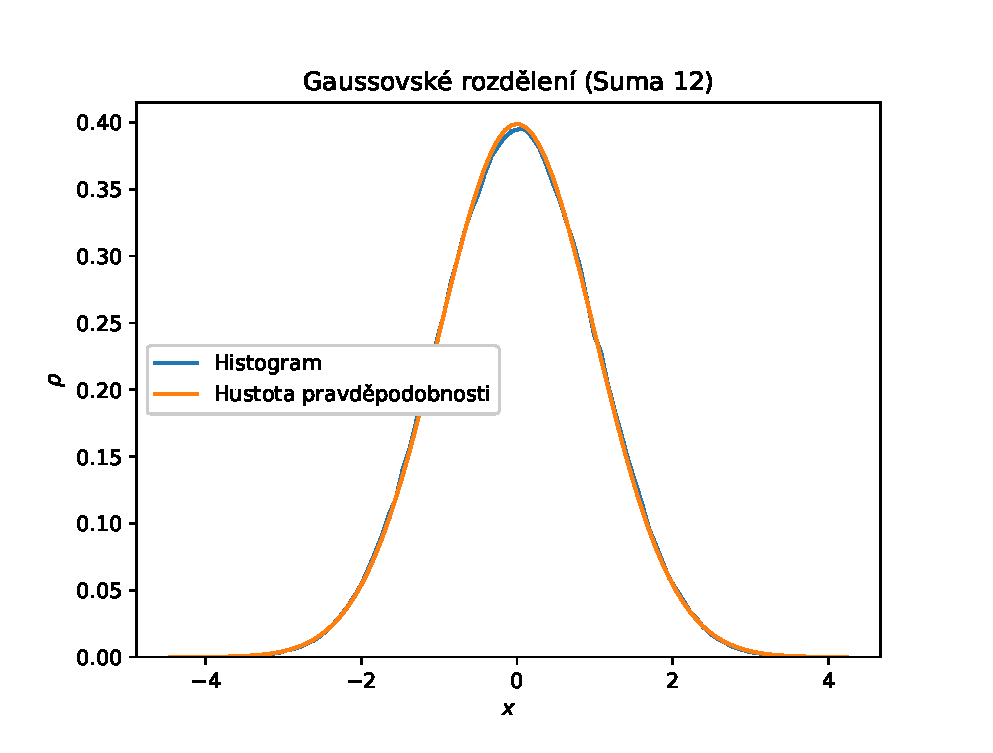
\epsfig{file=gaussian_sum12.eps,width=\linewidth}
                \caption{}
            \end{subfigure}
            \begin{subfigure}{0.49\linewidth}
                \centering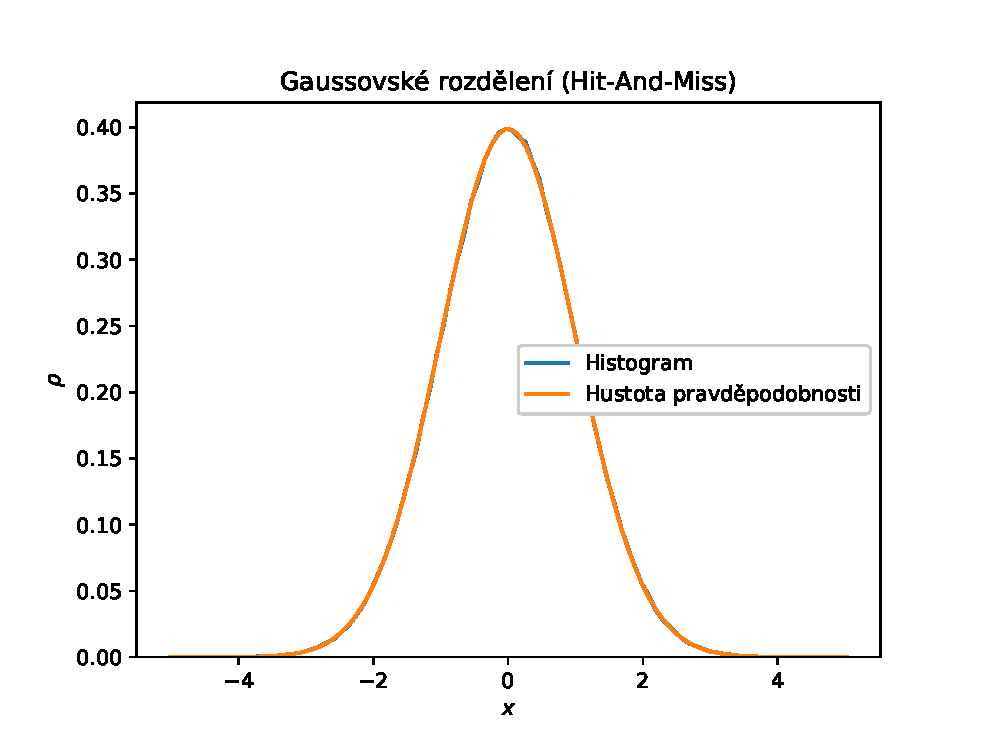
\epsfig{file=gaussian_hit_and_miss.eps,width=\linewidth}
                \caption{}
            \end{subfigure}
            \caption{
                \protect\small
                Srovnání jednoduchých generátorů Gaussovsky rozdělených náhodných čísel. 
                (a) Generátor založený na použití Centrální limitní věty~\eqref{eq:CLT1}: Gaussovské náhodné číslo je získáno jako součet $m=12$ rovnoměrně rozdělených náhodných čísel.
                (b) Generátor založený na hit-and-miss metodě použité na hustotu pravděpodobnosti Gaussovského rozdělení.
                V obou případech je pro zobrazovaný histogram použito  $n=10^{6}$ náhodných čísel a počet intervalů histogramu je $N=100$.
                U generátoru (a) je pozorována drobná odchylka v okolí maxima hustoty pravděpodobnosti, u generátoru (b) žádná odchylka pozorována není.
                Nutno zdůraznit, že generátor (a) je zhruba o řád rychlejší než generátor (b), jak je ukázáno v úloze~\ref{task:GeneratorTime}.
            }
            \label{fig:GaussianGenerator}
        \end{figure}    
    \end{solution}
    
    \begin{task}
        Nakreslete histogram pro rozdělení hodnot v jednotlivých intervalech histogramů z úlohy \ref{task:Distributions}.
        Jaké očekáváte statistické rozdělení v tomto případě?
    \end{task}

    \begin{solution}
        Počet hodnot v jednotlivých intervalech splňuje předpoklady pro Poissonovo rozdělení, očekáváme tedy Poissonovo rozdělení se parametrem
        \begin{equation}
            \lambda=\frac{\mathtt{num\_values}}{\mathtt{num\_bins}},
        \end{equation}
        který udává zároveň střední hodnotu~\eqref{eq:ExpectationP} a zároveň rozptyl~\eqref{eq:DispersionP}.
        Chceme-li toto rozdělení zobrazit, je potřeba jisté delikátnosti.
        \begin{itemize}
            \item 
                Počty hodnot v okénkách (nenormovaného) histogramu jsou přirozená čísla.
                Pro zobrazení jejich rozdělení je tedy vhodné volit sekundární histogram se šířkou intervalu 1 (nebo s jinou celočíselnou šířkou).
            \item
                Hezčí rozdělení získáme pro malé parametry $\lambda$ (pro $\lambda$ velké se Poissonovo rozdělení blíží Gaussovskému rozdělení).
                V kódu volím hodnoty tak, aby $\lambda=10$.
        \end{itemize}
        Srovnání příslušného histogramu s teoretickým rozdělením~\eqref{eq:Poisson} je vypočteno funkcí \code{poisson} ze souboru \ghfile{python/histogram/}{distributions.py} a je vykresleno na obrázku~\ref{fig:Poisson}.

        \begin{figure}[!htb]
            \centering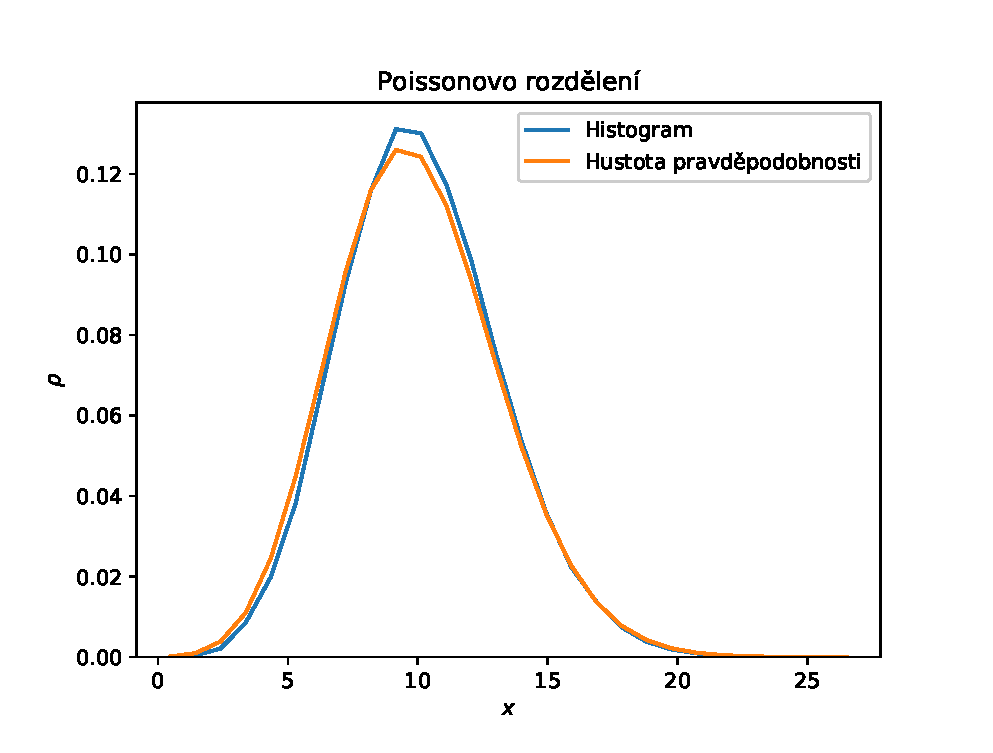
\epsfig{file=poisson.eps,width=0.6\linewidth}
            \caption{
                \protect\small
                Poissonovo rozdělení, získané z fluktuací počtu hodnot histogramu s $N=10^{5}$ intervaly a $n=10^{6}$ rovnoměrně rozdělenými vstupními čísly.
                Střední hodnota a rozptyl takto získaného Poissonova rozdělení je $\lambda=10$. 
            }
            \label{fig:Poisson}
        \end{figure}
    \end{solution}
    
    \begin{task}\label{task:GeneratorTime}
        Na základě známé hustoty pravděpodobnosti~\eqref{eq:NormalDistribution} vytvořte generátor čísel s Gaussovským normálním rozdělením.
        Porovnejte jeho rychlost s generátorem založeným na centrální limitní větě, který jste naprogramovali v úloze~\ref{task:NormalDistribution} a s generátorem z některé z knihoven.\footnote{Porovnání můžete provést tak, že nagenergujete větší množství čísel různými metodami, například $n=10^{6}$, a změříte dobu výpočtu.} 
    \end{task}

    \begin{solution}
        Generátor je naprogramován v souboru \ghfile{python/histogram/}{gaussian.py}, funkce \code{generator_hm}, a porovnání histogramu takto nagenerovaných náhodných hodnot s teoretickou hustotou pravděpodobnosti je na obrázku~\ref{fig:GaussianGenerator}(b). 
        Nagenerování $10^6$ Gaussovsky rozdělených náhodných čísel trvá na mém PC\footnote{
            Pokud k nagenerování $n$ hodnot použijeme knihovní funkci s počtem v argumentu, \code{generator.normal(1000000)}, výpočet trvá zlomek vteřiny.
            Velká část výpočetního času je tudíž způsobena voláním funkcí a prováděním cyklu. 
        }
        \begin{itemize}
            \item {\bf 4s}: funkce \code{generator.normal()} z knihovny \file{numpy},
            \item {\bf 16s}: součet 12 rovnoměrně rozdělených čísel,
            \item {\bf 111s}: hit-and-miss metoda.
        \end{itemize}
    \end{solution}

    \begin{task}
        Vytvořte generátor čísel z rozdělení daném distribuční funkcí
        \begin{equation}
            \label{eq:F}
            F(x)=\frac{1}{2}\left(1+\frac{2}{\pi}\arctan{x}\right).
        \end{equation}
        Jak vypadá analyticky hustota pravděpodobnosti?
        Nakreslete histogram a porovnejte.
    \end{task}

    \begin{solution}
        Hustota pravděpodobnosti je dána derivací distribuční funkce podle vztahu~\eqref{eq:rhoF}, tj.
        \begin{equation}
            \label{eq:Cauchy}
            \rho(x)=\derivative{F}{x}=\frac{1}{\pi}\derivative{}{x}\arctan{x}=\frac{1}{\pi}\frac{1}{1+x^{2}}.
        \end{equation}
        Toto rozdělní se nazývá \emph{Cauchyho} či v kvantové fyzice \emph{Breit-Wignerovo}. 
        Popisuje šířku energetických hladin exponenciálně se rozpadajících systémů.

        Ke generování čísel z tohoto rozdělení využijeme vztahu~\eqref{eq:xF}.
        Musíme tedy určit funkci inverzní k distribuční funkci~\eqref{eq:F}, která je
        \begin{equation}
            F^{-1}(y)=\tan\left[\frac{\pi}{2}\left(2y-1\right)\right],
        \end{equation}
        a za $y$ dosazovat čísla z rovnoměrného rozdělení na intervalu $\langle0,1\rangle$.

        Histogram čísel nagenerovaných z Cauchyho rozdělení a srovnání s hustotou pravděpodobnosti~\eqref{eq:Cauchy} je počítán funkcí \code{cauchy} souboru \ghfile{python/histogram/}{distributions.py} a je zobrazen na obrázku~\ref{fig:F}.
        Rozdělení má dlouhý dosah, s rostoucím $x$ klesá jen polynomiálně k nule, pravděpodobnost nagenerování hodnoty daleko od maxima je tudíž velká. 
        V obrázku proto zobrazuji jen okno $x\in\langle-10,10\rangle$.

        \begin{figure}[!htb]
            \centering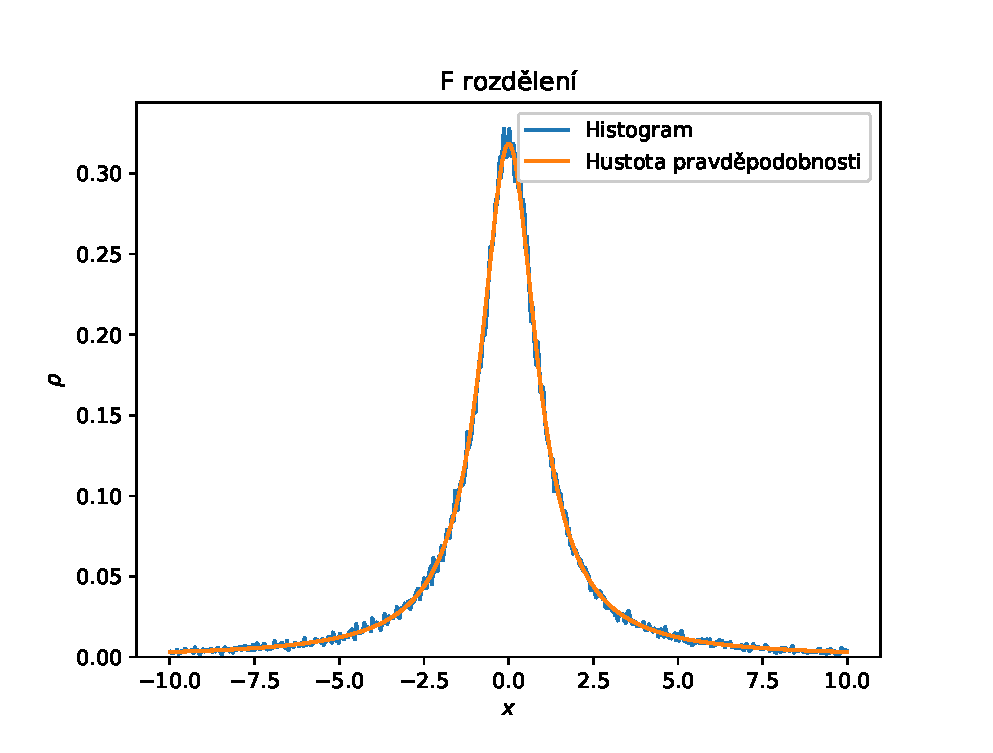
\epsfig{file=f.eps,width=0.6\linewidth}
            \caption{
                \protect\small
                Cauchyho (Breit-Wignerovo) rozdělení nagenerované z distribuční funkce~\eqref{eq:F} a porovnané s teoretickou hustotou pravděpodobnosti~\eqref{eq:Cauchy}.
                Počet hodnot pro histogram je $n=10^5$, počet intervalů $N=500$.
            }
            \label{fig:F}
        \end{figure}    
    \end{solution}

\section{Monte-Carlo metoda}
    Pod Monte-Carlo metodou se rozumí, že namísto systematického (a obvykle zdlouhavého) procházení nějakého parametrického prostoru využíváme náhodně generované body a hledané vlastnosti našeho systému určíme statisticky.\footnote{
        Monte Carlo je oblast Monaka, ve kterém se nacházely a doposud nacházejí slavná kasina.
        Odtud název.
    }
    V tomto cvičení zúročíme veškeré dosavadní zkušenosti s náhodnými čísly a budeme ze zabývat zejména integrací Monte-Carlo.

    Možná jste se již setkali se problémem tzv. \href{https://cs.wikipedia.org/wiki/Buffonova_jehla}{Buffonovy jehly}: pomocí náhodného házení jehly (či jakékoliv tyčky) na síť rovnoběžných čar nakreslenou na zemi lze určit číslo $\pi$, 
    \begin{equation}
        \pi\approx\frac{2l}{h}\frac{N_{\text{zásah}}}{N_\text{celkem}},
    \end{equation}
    kde $h$ je vzdálenost čar, $l\leq h$ délka jehly, $N_{\text{celkem}}$ celkový počet hodů a $N_{\text{zásah}}$ počet hodů, při kterých jehla po dopadu kříží nějakou z čar.
    Buffonova jehla je názorné experimentální použití metody Monte-Carlo, konkrétně varianty nazývané hit-and-miss.
    Té jsme se již dotkli v sekci~\ref{sec:SelectDistribution} a nyní si rozebereme podrobněji.
    
    \begin{task}
        Metodou Monte-Carlo vyřešte tzv. narozeninový problém: Uvažujte skupinu $n$ lidí. 
        Jaká je pravděpodobnost, že dva lidi ve skupině budou mít narozeniny ve stejný den?
        Úloha se samozřejmě dá vyřešit \href{https://cs.wikipedia.org/wiki/Narozeninov%C3%BD_probl%C3%A9m}{exaktně}, ale zkuste si úlohu vyřešit metodou Monte-Carlo:
        Pokud nagenerujete náhodně $N_{\text{celkem}}$-krát narozeniny $n$ lidí a označíte $N_{\text{zásah}}$ případy, kdy alespoň dvoje narozeniny padnou na stejný den, bude podle zákona velkých čísel hledaná pravděpodobnost rovna
        \begin{equation}
            p\approx\frac{N_{\text{zásah}}}{N_{\text{celkem}}}
        \end{equation}
        (rovnost by nastala pro $N_{\text{celkem}}\rightarrow\infty$).
        Naprogramujte tuto úlohu a určete,
        \begin{enumerate}
            \item jaká je pravděpodobnost pro skupinu $30$ lidí a
            \item jak velkou skupinu potřebujete, aby byla pravděpodobnost alespoň $30\%$.
        \end{enumerate}
    \end{task}

    \begin{solution}
        \begin{figure}[!htbp]
            \centering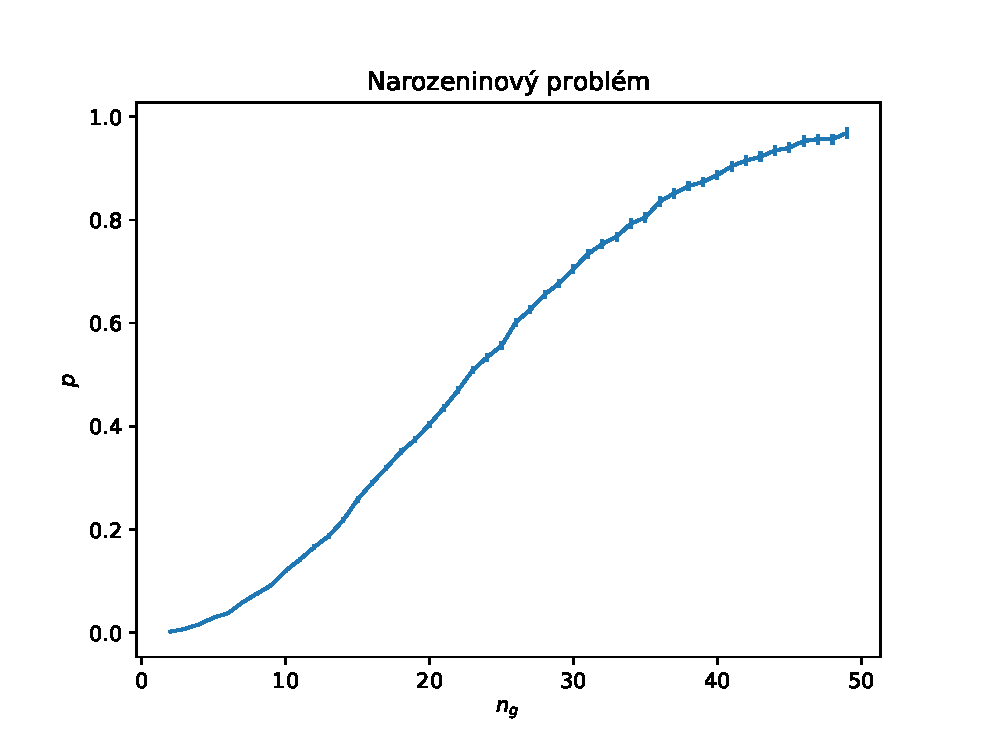
\epsfig{file=birthday_problem.eps,width=0.6\linewidth}
            \caption{
                \protect\small
                Pravděpodobnost, že ve skupině $n_{g}$ lidí budou mít alespoň dva lidé narozeniny ve stejný den v roce.
                Svislými čarami je odhad chyby $\pm1\sigma$.
                Počet pokusů pro metodu Monte-Carlo je $N_{\text{celkem}}=10^{4}$.
            }
            \label{fig:BirthdayProblem}
        \end{figure}

        Vzorové řešení je v souboru \ghfile{python/montecarlo/}{birthday.py} a obsahuje dvě funkce:
        \begin{itemize}
            \item \code{birthday_coincidence_probability} 
                určí metodou Monte-Carlo pravděpodobnost, že ve skupině o velikosti $n_{g}=\mathtt{group\_size}$ bude alespoň jedna dvojice, která slaví narozeniny ve stejný den v~roce.
                Řešení probíhá ve dvou krocích: 
                \begin{enumerate}
                    \item nagenergujeme řadu $n_{g}$ čísel mezi $1$ a $366$, které udávají den narozenin,\footnote{
                        Řešení počítá i s datem narození 29. února, přičemž předpokládá, že pravděpodobnost všech dat narození je stejná.
                        To však pro narozeniny 29. února neplatí, pravděpodobnost narození s tímto datem je menší, a to přibližně čtvrtinová.
                    }
                    \item zkontrolujeme, zda řada obsahuje dva stejné prvky (ve vzorovém řešení tak, že řadu seřadíme a zkontrolujeme, jestli obsahuje dvě či více stejných čísel v bezprostředně následujících prvcích).
                \end{enumerate}
                Funkce vrací hodnotu pravděpodobnosti $p$ a odhad chyby $\Delta p\approx1\sigma_{p}$.
            \item \code{plot_birthday_problem}
                vykreslí graf pravděpodobností pro interval velikostí skupin.
                Graf včetně chyb je na obrázku~\ref{fig:BirthdayProblem}.
        \end{itemize}
        
        Na základě těchto funkcí se jednoduše spočítá, že
        \begin{enumerate}
            \item Pro $n_{g}=30$ je pravděpodobnost $p\approx70\%$.
            \item Pro $n_{g}=17$ je pravděpodobnost $p\approx31\%$. 
        \end{enumerate}

        Program lze triviálně rozšířit a počítat například pravděpodobnost, že
        \begin{itemize}
            \item alespoň $d$ lidí bude mít narozeniny ve stejný den,
            \item alespoň $2$ lidé budou mít narozeniny ve stejný den i rok.
        \end{itemize}
    \end{solution}

    \subsection{Hit-And-Miss}
        Tato metoda spočívá v jednoduché aplikaci zákona velkých čísel.
        Její esence je načrtnuta na obrázku~\ref{fig:HitAndMiss}.
        Uvažujme nejprve, že chceme změřit plochu $s$ černého obrazce složitého tvaru znázorněného na panelu (a).
        Obrazec vepíšeme do jiného jednoduchého obrazce, jehož plochu $S$ známe (nejčastěji obdélník, případně kruh).
        Poté do tohoto obrazce $S$ náhodně \uv{házíme} body (křížky) a počítáme, kolikrát se trefíme do černého obrazce (červené křížky).
        Neznámá hledaná plocha $s$ je pak při již použitém značení
        \begin{equation}
            \label{eq:MCS}
            s\approx S\frac{N_{\text{zásah}}}{N_{\text{celkem}}}.
        \end{equation}

        \begin{figure}[!htbp]
            \begin{subfigure}{0.44\linewidth}
                \centering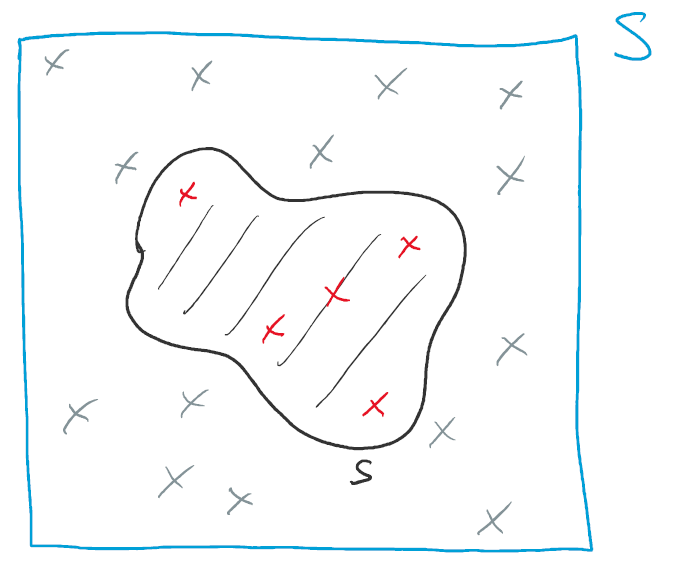
\includegraphics[width=\linewidth]{hit_and_miss.png}
                \caption{}
            \end{subfigure}
            \hfill
            \begin{subfigure}{0.54\linewidth}
                \centering\includegraphics[width=\linewidth]{hit_and_miss_int.png}
                \caption{}
            \end{subfigure}
            \caption{
                \protect\small
                Metoda hit-and-miss (a) pro výpočet plochy složitého obrazce a (b) pro výpočet integrálu jednorozměrné funkce.
                Podrobnosti k obrázku jsou uvedeny v textu. 
            }
            \label{fig:HitAndMiss}
        \end{figure}

        Analogicky postupujeme při integrování, což je ukázáno na panelu (b).
        Integrál v mezích $(a,b)$ je plocha pod křivkou funkce $f(x)$  (na obrázku černě vyšrafovaná plocha ohraničená zespodu osou $x$, shora funkcí $f(x)$ a ze stran modrými čarami $x=a$ a $x=b$).
        Uvedenou oblast vepíšeme do obdélníku o hranách $l=b-a$ a $h$ s plochou $S=(b-a)h$ a stejnou metodou jako u panelu (a) a pomocí stejného vzorce jako je~\eqref{eq:MCS} vypočítáme hodnotu integrálu:
        \begin{equation}
            \label{eq:MCSInt}
            \int_{a}^{b}f(x)\d x\approx S\frac{N_{\text{zásah}}}{N_{\text{celkem}}}=(b-a)h\frac{N_{\text{zásah}}}{N_{\text{celkem}}}.
        \end{equation}

        \subsubsection{Chyba}
            Počet zásahů je vlastně počet nezávislých \uv{hodů}, kterými se trefíme do oblasti, jejíž plochu $S$ hledáme.
            Pokud budeme opakovat metodu hit-and-miss s fixním $N_{\text{celkem}}$, bude mít náhodná veličina $N_{\text{zásah}}$ Poissonovo rozdělení se střední hodnotou~\eqref{eq:ExpectationP} a rozptylem~\eqref{eq:DispersionP}
            \begin{equation}
                \lambda=\expectation{N_{\text{zásah}}}=\dispersion{N_{\text{zásah}}}.
            \end{equation}
            Budeme-li mít jen jednu realizaci s dostatkem zásahů, můžeme střední hodnotu odhadnout pomocí této realizace, $\expectation{N_{\text{zásah}}}\approx N_{\text{zásah}}$ a absolutní chybu odhadneme směrodatnou odchylkou
            \begin{equation}
                \Delta N_{\text{zásah}}=\sqrt{\dispersion{N_\text{zásah}}}\approx\sqrt{N_{\text{zásah}}}.
            \end{equation}
            Relativní chyba pak je
            \begin{equation}
                \label{eq:MCRelative}
                \delta N_{\text{zásah}}=\frac{\Delta N_{\text{zásah}}}{N_{\text{zásah}}}\approx\frac{1}{\sqrt{N_{\text{zásah}}}}.
            \end{equation}
            Tento vzorec platí i pro relativní chybu ve výpočtu plochy~\eqref{eq:MCS} či integrálu~\eqref{eq:MCSInt}.

            Jelikož $N_{\text{zásah}}\propto N_{\text{celkem}}$, z uvedených úvah vyplývá, že
            \begin{itemize}
                \item relativní chyba klesá jako převrácená hodnota odmocniny celkového počtu pokusů $N_{\text{celkem}}$ a
                \item chceme-li zpřesnit výsledek získaný touto metodou desetkrát, musíme zestonásobit počet pokusů.
            \end{itemize}
            V praxi za použití běžných výpočetních prostředků lze dosáhnout nanejvýš $N_{\text{celkem}}\approx10^{10}$, což dá výsledek s relativní chybou minimálně $\delta\approx10^{-5}$, tj. pět desetinných míst.

        \subsubsection{Použití}
            Integrace pomocí metody hit-and-miss se nepoužívá, jelikož je příliš neefektivní. 
            K jejímu úspěšnému použití totiž musíme znát maximum funkce na zadaném intervalu, abychom efektivně určili výšku obdélníku $h$, a obecně je $N_{\text{zásah}}/N_{\text{celkem}}$ velmi malé číslo (funkce mají dlouhý chvost nebo jsou příliš vysoké), většina \uv{hodů} jde tedy mimo a i při jejich velkém množství získáme málo zásahů, a tudíž velkou chybu podle vztahu~\eqref{eq:MCRelative}.

            Na druhou stranu se tato metoda hodí k výpočtu povrchů, objemů či hyperobjemů v případě vícerozměrných objektů.
            
            \begin{task}
                Vytvořte program na výpočet objemu $d$-rozměrné jednotkové koule metodou Monte-Car\-lo.\footnote{
                    Pod $1$-rozměrnou jednotkovou koulí rozumíme úsečku délky 2, pod $2$-rozměrnou jednotkovou koulí jednotkový kruh.
                    Povrch jednotkového kruhu je $S=\pi$, výsledek lze tedy použít i k určení čísla $\pi$, aniž byste museli házet Buffonovou jehlou.
                }
                Pro jakou dimenzi bude tento objem největší číslo?
            \end{task}
        
            \begin{solution}
                Vzorový kód je v souboru \ghfile{python/montecarlo/}{ball.py}.
                Funkce \code{volume} spočítá objem jednotkové koule metodou Monte-Carlo a vrátí současně odhad chyby.
                Funkce \code{plot_volumes} vykreslí graf objemů v závislosti na dimenzi, jak je ukázáno na obrázku~\ref{fig:VolumeBall}.
                Nejvější objem $V\approx5.27$ dostaneme pro $d=5$.
                Zde je na místě jistá opatrnost: srovnáváme trochu \uv{jablka s hruškami}, protože samozřejmě objem různěrozměrných koulí má různou dimenzionalitu.
                Pro jiné než jednotkové koule tato závislost platit nebude.

                \begin{figure}[!htbp]
                    \centering\epsfig{file=volume_ball.eps,width=0.6\linewidth}
                    \caption{
                        \protect\small
                        Závislost objemu jednotkové koule na dimenzionalitě prostoru.
                        Svislými čarami je zobrazena chyba $\Delta V\approx1\sigma_{V}$.
                        Počet pokusů pro metodu Monte-Carlo je pro každý bod $N_{\text{celkem}}=10^{6}$.
                    }
                    \label{fig:VolumeBall}
                \end{figure}
    
                Z obrázku je rovněž vidět, že s rostoucím $d$ roste chyba výsledku.
                To je způsobeno tím, že s rostoucí dimenzionalitou se při metodě hit-and-miss čím dál častěji trefujeme mimo jednotkovou kouli, jinými slovy klesá při zadaném počtu pokusů počet zásahů.\footnote{
                    Pro $d=15$ je při $N_{\text{celkem}}=10^6$ počet zásahů pouze řádově $10^1$, tj. z každých sto tisíc pokusů se jen jednou trefíme do jednotkové koule, zbytek pokusů padá do \uv{rohů} opsaných krychlí.
                }
                Tento jev a jeho příčiny jsme již diskutovali v případě generování náhodného směru v $d$ dimenzích v řešení úlohy~\ref{task:NahodnaProchazka}.
            \end{solution}

    \subsection{Monte-Carlo integrace}
    \begin{figure}[!htbp]
        \begin{subfigure}{0.49\linewidth}
            \centering\includegraphics[width=\linewidth]{int1.png}
            \caption{}
        \end{subfigure}
        \hfill
        \begin{subfigure}{0.49\linewidth}
            \centering\includegraphics[width=\linewidth]{int2.png}
            \caption{}
        \end{subfigure}
        \caption{
            \protect\small
            Monte-Carlo integrace.
            Vysvětlení je v hlavním textu.
        }
        \label{fig:MCIntegral}
    \end{figure}

    Pro hledání integrálu je mnohem efektivnější metoda, již lze vysvětlit pomocí obrázku~\ref{fig:MCIntegral}.
    Uvažujme neprve, že známe pár hodnot $(x_{j},f(x_{j}))$, nic víc, nic míň.
    Na základě těchto hodnot můžeme učinit pouze velmi hrubý odhad integrálu, a to jako plochu červeně vyšrafovaného obdélníku jako na panelu (a),
    \begin{equation}
        \int_{a}^{b}f(x)\d x\approx (b-a)f(x_{j}).
    \end{equation}
    Pokud budeme mít párů hodnot $(x_{j},f(x_{j}))$ více, jak je znázorněno na panelu (b), vezmeme za odhad hodnoty integrálu průměr ploch takovýchto obdélníků,
    \begin{equation}
        \label{eq:MCInt}
        \int_{a}^{b}f(x)\d x
            \approx \frac{1}{N}\sum_{j=1}^{N}(b-a)f(x_{j})
            =\frac{b-a}{N}\sum_{j=1}^{N}f(x_{j}).
    \end{equation}
    V právě uvedeném postupu tkví je podstata integrace Monte-Carlo.
    Obecně platí, že pokud hodnoty $x_{j}$ vybíráme z rozdělení s hustotou pravděpodobnosti $\rho(x)$, je integrál odhadnutý výrazem
    \begin{equation}
        \int_{a}^{b}f(x)\d x
            \approx\frac{1}{N}\sum_{j=1}^{N}\frac{f(x_{j})}{\rho(x_{j})},
    \end{equation} 
    přičemž nejvhodnější je volit takové pravděpodobnostní rozdělení, jehož hustota pravděpodobnosti co nejlépe kopíruje integrovanou funkci.\footnote{
        Tento postup se nazývá \emph{importance sampling}.
    }
    V praxi, jelikož na funkci nejčastěji pohlížíme jako na \uv{černou skříňku} a o jejím průběhu nic nevíme, se jako nevhodnější jeví volit rovnoměrné rozdělení s hustotou pravděpodobnosti~\eqref{eq:UniformDistribution}, která po dosazení dá předchozí vzorec~\eqref{eq:MCInt}.

    Chybu metody integrace lze odhadnout pomocí směrodatné odchylky
    \begin{align}
        \Delta\equiv\sigma&=\sqrt{\overline{f^{2}}-\overline{f}^{2}},\\
        \overline{f^{2}}&=\frac{1}{N}\sum_{j=1}^{N}f^{2}(x_{j}),\nonumber\\
        \overline{f}^{2}&=\left[\frac{1}{N}\sum_{j=1}^{N}f(x_{j})\right]^{2}.\nonumber
    \end{align}

    \begin{task}
        Metodou Monte-Carlo spočítejte integrály
        \begin{align}
            I_{1}&\equiv\int_{0}^{2\pi}\e^{-x}\sin{x}\,\d x,
            \label{eq:I1}\\
            I_{2}&\equiv\int_{0}^{\sqrt{10\pi}}\frac{\sin{x^{2}}}{\sqrt{1+x^{4}}}\d x.
        \end{align}
        První integrál má analytické vyjádření, které si můžete odvodit a porovnat s hodnotou získanou Monte-Carlo integrací; druhý integrál lze spočítat pouze numericky.
        Metodu můžete otestovat i na jiných známých integrálech.
    \end{task}

    \begin{solution}
        Řešení je naprogramováno v souboru \ghfile{python/montecarlo/}{integration.py} dvěma způsoby:
        \begin{enumerate}
            \item \code{integrate_1D} 
                integruje postupným generováním $N=\mathtt{n}$ náhodných bodů a výpočtem pomocí rovnice~\eqref{eq:MCInt}.
            \item \code{integrate_1D_array} 
            nageneruje řadu $N$ bodů z intervalu $\langle a,b\rangle$, pro tuto řadu spočítá řadu funkčních hodnot a tu pak sečte a vynásobí příslušným prefaktorem, rovněž dle rovnice~\eqref{eq:MCInt}.
            Tento postup je výrazně rychlejší, neboť obsluha cyklů a volání funkcí pro individuální body stojí v interpetovaných jazycích (jímž Python je) velké množství výpočetního času.
            Na druhou stranu tento postup vyžaduje mít v operační paměti uložená dlouhá pole bodů $x_{j}$ a $f(x_{j})$ a pro velké počty $N$ nám dostupná paměť nemusí stačit.
            Řešením je samozřejmě oba postupy zkombinovat. 

            Výsledky integrálů jsou
            \begin{align}
                I_{1}&=\frac{1}{2}\left(1-\e^{-2\pi}\right)\approx0.499,\\
                I_{2}&\approx0.493.
            \end{align}
        \end{enumerate}
    \end{solution}

    Síla metody Monte-Carlo se naplno projeví při výpočtu vícerozměrných integrálů.
    Jak bylo ukázáno, chyba metody závisí jen na celkovému počtu pokusů $N=N_{\text{celkem}}$.
    Zatímco u jiných metod při požadování určité dané přesnosti výsledku drasticky narůstá časová složitost integrace s rostoucí dimenzí integrované funkce, u Monte-Carla časová složitost na dimenzi závisí jen nepatrně.
    Ve více rozměrech bývá navíc integrační oblast složitější, k čemuž lze využít metodu hit-and-miss.
    To se nejlépe ukáže na příkladu.

    \begin{task}\label{task:I3}
        Spočítejte čtyřrozměrný integrál
        \begin{equation}
            I_{3}\equiv\int_{\Omega}\sin{\sqrt{\ln\left(x+y+z+w+2\right)}}\,\d x\,\d y\,\d z\,\d w,
            \label{eq:I3}
        \end{equation}
        kde integrační oblast je hyperkoule
        \begin{equation}
            \Omega: \left(x-\frac{1}{2}\right)^{2}+\left(y-\frac{1}{2}\right)^{2}+\left(z-\frac{1}{2}\right)^{2}+\left(w-\frac{1}{2}\right)^{2}\leq\frac{1}{4}.
        \end{equation} 
        Při výpočtu postupujte tak, že nejprve danou hyperkouli vepíšete do hyperkvádru (či hyperkrychle) známých rozměrů, a tudíž známého objemu $V$.
        Poté pro náhodně zvolený bod v hyperkvádru určíte, zda se trefí do hyperkoule $\Omega$ či nikoliv.
        Pokud ano, spočítáte funkční hodnotu integrandu v tomto bodě.
        Jedná se tedy o kombinaci integrace~\eqref{eq:MCInt} a metody hit-and-miss.
        Budete-li si uchovávat počet hodů $N_{\text{celkem}}$ a počet zásahů $N_{\text{zásah}}$, získáte jako vedlejší produkt objem integrační hyperoblasti pomocí vzorce~\eqref{eq:MCS}.
    \end{task}

    \begin{solution}
        Řešení pro tento konkrétní integrál je naprogramováno v souboru \ghfile{python/montecarlo/}{integration.py} ve funkci \code{integral3}.
        Pro $N_{\text{celkem}}=10^{6}$ tento integrál vychází přibližně
        \begin{equation}
            I_{3}\approx0.284.
        \end{equation}
        Funkce \code{integral_ND} pak obsahuje obecnější řešení, které integruje libovolnou funkci v libovolněrozměrném prostoru na funkcí $\code{is_inside_region}$ zadané integrační oblasti.
    \end{solution}

    
    \section{Paralelizace}
    Rychlost výpočtu lze v zvyšovat dvěma základními způsoby:
    \begin{enumerate}
        \item Zvyšováním rychlosti procesoru.
        \item Zvětšováním počtu procesorů.
    \end{enumerate}
    Zatímco první způsob již narazil na fyzikální limity a kupředu postupuje jen zvolna,\footnote{
        Maximální dosažitelná rychlost procesorů je dnes přibližně $5$ GHz, tj. řádově miliardy strojových cyklů za vteřinu, a během posledních let se nemění. 
        Strojová instrukce většinou trvá několik cyklů a jejich provádění je navíc zpomalováno přístupem programu do operační paměti, proto dnešní procesory zvládnou řádově nanejvýš stovky milionů instrukcí za vteřinu.
        Jeden jednoduchý příkaz v Pythonu může vyžadovat stovky až tisíce procesorových instrukcí, takže Python vykoná řádově maximálně stovky tísíc příkazů za vteřinu.
        Ke zrychlení procesoru se využívají nejrůznější sofistikované metody. 
        Procesor například odhaduje, kam se program vydá, a instrukce se snaží předpočítávat dopředu. 
        Pokud se v odhadu trefí, dojde ke zrychlení.
        Jiný způsob je vytváření nových strojových instrukcí, které zrychlují určitý často používaný typ úloh (například instrukce rychlá Fourierova transformace, která se intenzivně používá při dekódování videa a při práci s obrázky).
    } 
    druhý způsob lze použít takřka neomezeně.
    V dnešní době mají procesory osobních počítačů, ale i mobilních telefonů či dalších zařízení běžně dva až čtyři plnocenné podprocesory nazývané jádra, přičemž některé procesory navíc umožňují na každém jádře spustit dvě vlákna (technologie \emph{hyperthreading}\footnote{
        Technologie spočívá v tom, že v každém procesorovém jádře jsou různé výpočetní jednotky, které zpracovávají různé typy procesorových instrukcí.
        Zatímco se tedy v jednom vlákně násobí dvě čísla s desetinnou čárkou, v jiném vlákně na tomtéž jádře se může zpracovávat například cyklus přes celočíselný index.
    }).
    To znamená, že můžeme na procesoru spustit několik výpočtů najednou a výpočty budou probíhat paralelně.
    
    Jeden probíhající výpočet se běžně nazývá \emph{vlákno} (thread) nebo \emph{proces}.\footnote{
        Ve skutečnosti je to složitější, jeden proces může obsahovat i více vláken, ale v těchto zápiscích budu předpokládat, že v každém procesu běží jen jedno vlákno, a tudíž budu obě označení brát jako synonyma.
    }
    V moderních operačních systémech je počet současně běžících procesů neomezený.
    Pokud je procesů více, než dostupných procesorových jader, tak operační systém velmi rychle přepíná mezi prováděním procesu, čímž se zdá, že všechny procesy probíhají zároveň (tzv. \emph{preemptivní multitasking}).
    Přepínání samozřejmě stojí určitý výpočetní čas.
    Optimální situace tedy je, pokud se počet procesů přesně rovná počtu procesorových jader.\footnote{
        We Windows se počet jader nejsnáze zjistí pomocí Správce úloh (Task manager), který lze vyvolat například stiskem kláves~\code{Ctrl+Shift+Esc}.
    }
    Pak jsou všechna jádra vytížena, a přitom operační systém není zatěžován nutností přepínat mezi jednotlivými vlákny. 
    Toto je demonstrováno na obrázku~\ref{fig:Duration}.
    
    Nejtriviálnější způsob paralelizace spočívá v tom, že spustíme nezávisle více programů najednou.
    Operační systém automaticky využije veškerá dostupná procesorová jádra.
    My jen počkáme na výsledky a ty pak zpracujeme.
    Tento způsob vpodstatě vylučuje jakoukoliv komunikaci mezi jednotlivými vlákny, a úlohy proto musejí být zcela nezávislé.
    Z vnějšku lze také jen velmi omezeně řídit provádění vláken, například spustit nový výpočet po doběhnutí konkrétního vlákna. 

    Pokročilejší postup je ten, kdy danou úlohu rozsekáme na nezávislé samostatné úseky, ty pak z našeho programu (tzv. \emph{hlavního vlákna}) pošleme ke zpracování na více procesorů, počkáme na výsledky a ty následně zpracujeme.
    Takto lze jednoduše paralelizovat metodu Monte-Carlo: výpočet $N$ Monte-Carlo bodů spustíme současně v $p$ vláknech, a poté všechny výpočty spojíme dohromady tak, že jednoduše spočítáme aritmetický průměr výsledků jednotlivých vláken, přičemž tato hodnota odpovídá jednomu Monte-Carlo výpočtu s $pN$ body.
    Jednotlivá vlákna výpočtu se sebou nemusejí nijak komunikovat, nemusejí sdílet žádnou část paměti, není tudíž potřeba řešit jejich vzájemnou sychronizaci (v anglické terminologii se pro takovýto typ problémů používá označení \uv{embarassingly parallel}, trapně paralelní).\footnote{
        Ve striktně funkcionálním programování není dovoleno funkcím měnit hodnoty proměnných, a proto lze čistě funkcionální programy triviálně paralelizovat.
    }
    
    V úplně obecném případě je nutné řešit vzájemnou sychronizaci vláken, což přesahuje rámec tohoto kurzu. 
    Pro ilustraci uvedu jen jeden z nejzákladnějších příkladů: 
    Představte si, že dvě vlákna sdílejí některé proměnné, a tedy přistupují do stejné části paměti. 
    Pak je nutné zabránit tomu, aby obě vlákna k jedné proměnné přistupovala zároveň (například jedno z proměnné četlo, zatímco druhé do ní zapisovalo).
    To by totiž vedlo k nejednoznačnému výsledku, protože nelze a priori říci, které vlákno bude operaci provádět dříve. 
    K vyřešení kolize se používají tzv. \emph{zámky} (lock).
    Než vlákno přistoupí ke sdílené proměnné, zamkne si ji pro sebe, provede svoji operaci a poté proměnnou odemkne.
    Pokud by mezitím k zamčené proměnné chtělo přistoupit jiné vlákno, jeho provádění se zastaví a vlákno čeká, než bude proměnná odemčena.
    Z toho ihned vyplývá, že při velkém počtu sdílených proměnných či při častém přístupu k nim dochází k významnému zpomalení paralelního zpracování, neboť velkou část výpočetního času vlákna čekají na přístup k momentálně zamčeným proměnným.

    Zamykání proměnných s sebou nese problémy a potenciální obtížně odhalitelné chyby.
    Může se stát, že zapomeneme proměnnou odemknout, čímž zastavíme všechna ostatní vlákna, která chtějí k proměnné přístupovat.
    K zablokování programu může dojít i tak, že provádění vlákna skončí chybou ve chvíli, kdy má pro sebe nějakou proměnná zamčenou. 

    Jiný možný způsob zablokování paralelního výpočtu kvůli zámkům je tzv. \emph{gridlock}: Jedno vlákno chce například sečíst hodnotu proměnných \code{a} a \code{b}.
    Zamkne proměnnou \code{a} a chce zamknout i proměnnou \code{b}, avšak tu má zrovna zamčenou druhé vlákno.
    Pokud v tu chvíli druhé vlákno potřebuje přistoupit k proměnné \code{a}, není mu to povoleno, protože tato proměnná je zamčena prvním vláknem.
    První vlákno tedy čeká na odemčení proměnné \code{b} aby mohlo odemknout proměnnou \code{a}, zatímco to druhé na odemčení proměnné \code{a}, bez čehož neuvolní proměnnou \code{b}. 
    Obě vlákna jsou do sebe zakleslá, čekají a k uvolnění nedojde nikdy.    

    Pro pěkný podrobný úvod do paralelního programování doporučuji \url{https://hpc.llnl.gov/documentation/tutorials/introduction-parallel-computing-tutorial}.

    V Pythonu existují dvě základní knihovny pro zpracování programu ve více vláknech: \file{\href{https://docs.python.org/3/library/threading.html}{threading}} a \file{\href{https://docs.python.org/3/library/multiprocessing.html}{multiprocessing}}.
    První z nich obsahuje více funkcionalit, avšak spouští všechna vlákna jen na jednom procesoru (jádře), k paralelnímu provádění výpočtů se tedy nehodí.\footnote{
        Použití knihovny \file{threading} je vhodné v případě, kdy provádíme úlohy, ve kterých se obvykle čeká na výsledek.
        Chceme například stáhnout webovou stránku z nějakého serveru, což může trvat nedefinovaně dlouho, a nechceme přitom, aby náš program přestal po dobu čekání reagovat.
    }

    Paralelizace na více výpočetních jádrech je v Pythonu implementována v knihovně \file{\href{https://docs.python.org/3/library/multiprocessing.html}{mul\-ti\-pro\-ces\-sing}}.
    Zde si ukážeme využití objektů \code{Pool}, \code{Process} a \code{Value} z této knihovny na příkladu paralelní integrace metodou. Monte-Carlo.
    Vzorový kód je naprogramován v souboru \ghfile{python/montecarlo/}{parallelization.py}.
    \begin{itemize}
        \item \code{integrate_1D_Pool}:
            Nejjednodušší způsob paralelizace je pomocí objektu \code{Pool}. 
            Při vytváření instance tohoto objektu mu předáme parametr \code{processes} udávající maximální počet procesů, které bude objekt obsluhovat.\footnote{
                Pokud parametr \code{processes} nezadáme, Python použije všechna dostupná jádra procesoru, dostupná také v globální proměnné \code{os.cpu\_count()}.
            }
            Následně zavoláme jeho metodu \code{starmap}, jejíž první parametr je funkce, kterou chceme spustit v jednotlivých procesech, a druhý parametr je seznam, jehož každý element obsahuje n-tici s argumenty naší funkce.
            Metoda \code{starmap} spustí postupně naši funkci se všemi dostupnými n-ticemi parametrů ze seznamu, přičemž použije všechny dostupné procesy objektu \code{Pool},
            počká na výsledky z jednotlivých vláken a shromáždí je do seznamu, který přiřazujeme proměnné \code{results}.\footnote{
                Pokud je n-tic s argumenty víc než počet dostupných procesů, bude objekt \code{Pool} spouštět volání postupně.
            }
            Průměr ze všech hodnot dá finální hodnotu integrace Monte-Carlo.

            Pokud by naše funkce měla jen jeden argument, namísto metody \code{starmap} bychom použili jednodušší metodu \code{map}.
            Ve vzorovém příkladu však spouštěné funkci \code{integrate_1D} musíme předat argumenty čtyři, proto volíme složitější \code{starmap}.

            Při vytvoření instance objektu \code{Pool} jsme použili konstrukci s klíčovým slovem \code{with}.

        \item \code{integrate_1D_process}:
            Složitější, avšak univerzálnější je použití objektů \code{Process}.\footnote{
                Podobným způsobem se používá knihovna \file{pthread} v programovacím jazyce C++.
            }
            Ty vyžadují vykonání tři kroků:
            \begin{enumerate}
                \item 
                    Vytvoříme instanci objektu typu \code{Process}.
                    Při tom musíme specifikovat parametr \code{target}, jímž předáme funkci, kterou chceme v procesu spustit, a parametr \code{args}, který obsahuje její argumenty.
                \item
                    Výpočet v procesu spustíme pomocí metody \code{start}.
                    Výpočet se spustí asynchronně, naše hlavní vlákno programu tedy nečeká, než se výpočet v novém procesu dokončí.
                \item
                    Chceme-li počkat na výsledek, využijeme metodu \code{join}.
                    Zavoláme-li ji pro daný proces, bude hlavní vlákno programu čekat na dokončení příslušného procesu.
                    My chceme počkat na dokončení všech procesů, proto si musíme po vytvoření a nastartování procesy uschovat (ve vzorovém kódu je uschováváme v proměnné \code{processes}) a poté zavolat \code{join} pro všechny.
            \end{enumerate}

            Při použití objektu \code{Process} {\bf není možné získat návratovou hodnotu volané funkce}.
            Proto musíme program ještě trochu zesložitit a volanou funkci vrátit ve sdílené proměnné --- instanci objektu \code{Value}.
            Tento objekt slouží k přenosu hodnot mezi hlavním vláknem a ostatními procesy i mezi procesy navzájem.
            První parametr při vytváření instance objektu \code{Value} udává typ (\code{'d'} pro číslo s desetinnou čárkou, \code{'i'} pro celočíselný typ), druhý parametr počáteční hodnotu.
            Hodnota proměnné je uložena v atributu \code{value}.
            Vytvoříme takovouto proměnnou pro každý jednotlivý proces.
            Navíc musíme naprogramovat pomocnou funkci (\emph{wrapper}), kterou pojmenujeme \code{integrate_1D_parallel}  a která nám zavolá naši funkci \code{integrate_1D} a její návratovou hodnotu uloží do sdílené proměnné.
            Naší funkci \code{integrate_1D} chceme předat beze změny všechny parametry, které pomocná funkce \code{integrate_1D_parallel} dostane.
            K tomu slouží konstrukce \code{*args, **kwargs}.
            
            Objekt \code{Value} má v sobě implementovaný zámek.
            Stačilo by tedy použít jen jednu instanci \code{Value} pro všechny procesy a výsledky dílčích integrací do ní přičítat.
            Průměr bychom nakonec získali vydělením počtem procesů.
    \end{itemize}

    \begin{figure}[!htb]
        \begin{subfigure}{0.49\linewidth}
            \centering\epsfig{file=multiprocessing_time_total.eps,width=\linewidth}
            \caption{}
        \end{subfigure}
        \hfill
        \begin{subfigure}{0.49\linewidth}
            \centering\epsfig{file=multiprocessing_time.eps,width=\linewidth}
            \caption{}
        \end{subfigure}
        \caption{
            \protect\small
            Výpočetní čas integrace metodou Monte-Carlo při použití různého počtu paralelních procesů $p$, přičemž v každém vlákně je spuštěn výpočet integrálu $I_{1}$~\eqref{eq:I1} s $N=10^{6}$.
            Výpočet byl prováděn na PC se 4-jádrovým procesorem Intel se zapnutou technologií hyperthreading.
            Celková doba výpočtu je $T$, doba výpočtu vztažená na jádro je $t\equiv T/p$.
            Pozorujeme, že celková doba výpočtu se pro $p\leq4$ téměř nemění, protože každý proces běží na svém vlastním jádře.
            Pro $4\leq p\leq8$ začíná narůstat celkový výpočetní čas, protože procesy se již musejí dělit o dostupná jádra, avšak výpočetní čas na vlákno stále nepatrně klesá díky hyperthreadingu.
            Pro $p\geq8$ se již procesor saturuje a zvětšování počtu procesů nepřináší žádný efekt.
            Pro $p\gg8$ bychom pozorovali naopak zhoršování času výpočtu na vlákno, protože by si pro sebe více a více výpočetního času brala režie operačního systému, aby všechna vlákna obhospodařila.
        }
        \label{fig:Duration}
    \end{figure}

    {\bf Důležité poznámky:}
    \begin{itemize}
        \item
            Python postupuje tak, že v jednotlivých procesech spouští celé moduly obsahující spouštěnou funkci.
            V našem případě je v každém procesu spuštěn celý modul \ghfile{python/montecarlo/}{parallelization.py}.
            Tento modul obsahuje globální část kódu, která v našem případě spouští funkce, které spouštějí víceprocesorové zpracování, a došlo by tedy k zacyklení programu.
            Abychom tomuto zabránili, je nutné tu část kódu, která smí být spuštěna jen z hlavního vlákna, vložit do podmínky\\
            \code{if \_\_name\_\_ == "\_\_main\_\_":}

        \item
            Ve Windows ve vývojovém prostředí IDLE nefunguje funkce \code{print}, pokud ji používáme z jiného než z hlavního vlákna (nic nevypíše).
            V jiných prostředích či operačních systémech by to mělo fungovat.
    \end{itemize}

    Efekty paralelizace lze vidět pomocí funkce \code{plot_integrate_1D_duration}.
    Tato funkce spouští postupně paralelní výpočet pro různé počty navzájem běžících paralelních vláken,
    a výsledky zobrazí do grafů, které jsou vykresleny v obrázku~\ref{fig:Duration}.  
    Pozorujeme, že nejlepší přesnosti (nejvyššího poštu Monte-Carlo bodů $pN$) za jednotku času dosáhneme, pokud vytížíme všechna dostupná jádra. 

    \newpage
    \subsection{Domácí úkol na 4.5.2021}
    \begin{task}
        Prostudujte si vzorový příklad v souboru \ghfile{python/montecarlo/}{parallelization.py} a na jeho základě vytvořte kód, který bude počítat ve více vláknech hodnotu integrálu $I_{3}$~\eqref{eq:I3} z úkolu~\ref{task:I3}.
        Zjistěte si, kolik výpočetních jader má procesor na vašem počítači, a spusťe výpočet tak, aby zaměstnal všechna jádra.
    \end{task}

    \begin{task}
        Časově náročný, a přitom jednoduše paralelizovatelný je výpočet součinu dvou matic.
        Jelikož metoda \code{starmap} pracuje jednoduše jen s vektory, naprogramujte paralelní výpočet součinu matice a vektoru (výsledkem je vektor).
    \end{task}

    \section{LaTeX}
    Nedílnou součástí vědecké práce je prezentování výsledků, přičemž chceme, aby dokument bylo jednoduché napsat, a zároveň aby dobře vypadal.
    Jelikož fyzikální odborné texty obsahují velké množství rovnic a symbolů, není nejvhodnější volbou používat textové editory pro kancelářskou práci, jejichž možnosti psaní rovnic a použití vědeckých stylů jsou celkem omezené.
    Ve fyzice je nejběžnější psát texty v systému \LaTeX. 
    
    Dnes se jedná o nesmírně obsáhlý balík různých knihoven a doplňků, pomocí kterého lze
    \begin{itemize}
        \item psát dobře vypadající a typograficky správné odborné texty s matematickými rovnicemi, obrázky a tabulkami,
        \item vybírat z množství profesionálně připravených stylů obsahujících podporu tvorby obsahu, rejstříku, poznámek pod čarou, kapitol, seznamů, referencí a dalších vychytávek,
        \item stáhnout si přímo styl časopisu či knihy, pro kterou text připravujeme, 
        \item používat tisíce matematických symbolů či druhů písem (lze psát třeba ve švabachu, gotickém písmu či elfím písmu, jste-li fanoušci díla J.R.R. Tolkiena),
        \item využívat různá makra a doplňky k jednoduchému vytváření speciálních objektů (například chemických vzorců nebo Feynmannových diagramů),
        \item vytvářet robustní prezentace (například pomocí knihovny Beamer),
        \item nebo sázet notové materiály a kdovíco dalšího (rajčata však zatím ne).
    \end{itemize}

    Systém \LaTeX{} má dvě vrstvy:
    \begin{enumerate}
        \item \TeX{}: sazeč (zajišťuje, aby vše bylo na stránce tam, kde má být),
        \item \LaTeX{}: typograf (zajišťuje, aby dokument dobře vypadal).
    \end{enumerate}
    Program \TeX{} začal vznikat v 70. letech 20. století a byl určen sázení textu a matematických rovnic při zachování vysoké typografické úrovně výsledného dokumentu.
    \LaTeX{} je pak nadstavba maker, která psaní dokumentů velmi zjednodušuje a zcela zakrývá sazečskou práci. 
    Příkazy v \TeX{}u jsou však stále dostupné.

    Dokument napsaný v \LaTeX{}u striktně odděluje \emph{text} (obsah) a \emph{styl} (vzhled), přičemž my využijeme standardní \LaTeX{}ovský styl a budeme se zabývat výhradně tím, jak napsat text.
    Jeho psaní se podobá programování: zdrojový soubor je textový dokument (nebo soubor textových dokumentů), který sestává z našeho textu a doplňujících příkazů.
    Chceme-li vidět, jak bude výsledný dokument vypadat, musíme soubor \uv{přeložit}.

    Existují různé \emph{distribuce} \LaTeX{}u.
    Jedna z nejpoužívanějších je \href{https://miktex.org/}{MiKTeX}.
    Dále je nutné mít k~dispozici textový editor, přičemž vhodný je ten, který rozumí \TeX{}ovským příkazům a bude umět zdrojový text poslat k překladu a zobrazit.
    Pokročilé editory umějí navigovat mezi zdrojovým textem k přeloženému výsledku (většinou do PDF souboru) a naopak.
    Z volně dostupných editorů jsou nejčastěji používané:
    \begin{itemize}
        \item {\bf TeXworks}: 
            Editor se základními funkcemi. Je součástí distribuce MiKTeX.
        \item \href{https://www.texniccenter.org/}{TeXnicCenter}: 
            Pokročilejší editor, podpora použití projektů.
        \item \href{https://www.texstudio.org/}{TeXstudio}: 
            Pokročilý editor, podpora projektů, automatického doplňování, jednoduchá práce s obrázky, možnost tvorby záložek, pomocníci po tvorbu rovnic a tabulek, zvýrazňování syntaktických chyb.
        \item \href{https://code.visualstudio.com/}{Visual Studio Code} s pluginem \href{https://marketplace.visualstudio.com/items?itemName=James-Yu.latex-workshop}{LaTeX Workshop}: 
            Méně funkcí co se týče samotného \LaTeX{}u a komplikovanější instalace, avšak plná podpora všech funkcí tohoto rozšířeného vývojového prostředí (integrace s Gitem, pokročilé vyhledávání, programátorské možnosti editace).
            Pro správnou funkci je nutné kromě uvedeného doplňku nainstalovat ještě interpret jazyka \href{https://www.perl.org/}{PERL}.
            Ve VS Code vznikají i tyto zápisky.
        \item \href{https://www.overleaf.com/}{Overleaf}: Online editor, ideální pro práci v týmu. 
            Nemusíte nic instalovat, potřebujete však připojení k internetu. 
            Pro větší projekty je nutná placená verze.
    \end{itemize}

    \begin{task}
        Nainstalujte si na svůj počítač nějakou distribuci \LaTeX{}u a editor.
    \end{task}

    \subsection{Formát \TeX{}ovského souboru}
    \begin{itemize}
        \item ASCII nebo UTF-8 kódování (lze použít i obskurnější kódování, ale v dnešní době je UTF-8 dostatečně univerzální).
        \item \emph{Mezery}: více mezer je interpretováno jako jedna mezera, jednoduché zalomení řádku také jako jedna mezera.
        \item \emph{Nový odstavec}: dvě zalomení řádku po sobě.
        \item \emph{Příkazy}: uvozeny znakem \verb+\+, jejich povinné parametry ve složených závorkách \verb+{...}+, volitelné parametry v hranatých závorkách \verb+[...]+.
            U názvů příkazů záleží na velikosti písmen.
        \item \emph{Rovnice v textu}: oddělena znaky \verb+$...$+. Některé příkazy lze použít pouze uvnitř rovnic, jiné naopak uvnitř rovnic použít nelze.
        \item \emph{Komentář}: uvozen znakem \verb+%+. Vše za tímto znakem až do konce řádky je ingnorováno.
    \end{itemize}

    \subsection{Struktura \TeX{}ovského souboru}
        \subsubsection{Preambule}
            Jedná se o první řádky souboru, než začne vlastní tělo dokumentu.
            Obsahuje výčet všech použitých balíčků a parametry, které se použijí pro styl textu.
            \begin{itemize}
                \item \verb+\documentclass[a4paper,twoside,11pt,twocolumn]{article}+: Základní specifikace stylu dokumentu (v tomto případě papír velikosti A4, dvoustránkový tisk, základní velikost písma 11 bodů, dvousloupcová sazba).
                Tento příkaz je povinný, musí být vždy přítomen.

                \item \verb+\usepackage{epsfig}+: Použije se balíček \verb+epsfig+.
                
                \item \verb+\def\abs#1{\left|#1\right|}}+: Definuje makro \verb+\abs+ s jedním parametrem (absolutní hodnota).
            \end{itemize}

            Nejčastěji používané balíčky jsou tyto:
            \begin{itemize}
                \item \verb+\usepackage{amsfonts,amsmath,amssymb}+:\footnote{AMS $=$ American Mathematical Society.} Rozšiřuje množství použitelných písem, matematických symbolů a struktur (např. snazší psaní matic, víceřádkových rovnic atd.).

                \item \verb+\usepackage[utf8]{inputenc}+: Specifikuje UTF-8 jako vstupní kódování (jinak je očekáváno ASCII).
            
                \item \verb+\usepackage[czech]{babel}+: Udávající české formátování (například české uvozovky) a české názvy (například Obsah, Rejstřík).

                \item \verb+\usepackage{epsfig}+: Umožní vkládání vektorových EPS souborů.

                \item \verb+\usepackage[unicode]{hyperref}+: Umožní vkládání hypertextových odkazů a učiní klikabilní i odkazy na rovnice, obrázky, stránky či kapitoly v textu pro snazší navigaci. 

            \end{itemize}

        \subsubsection{Tělo dokumentu}
            Tělo je uvozeno příkazy
            \begin{verbatim}
        \begin{document}
            ...
        \end{document}
            \end{verbatim}
            a do něj píšeme vlastní text dokumentu.
            Vše, co se nachází za příkazem \verb+\end{document}+, je ignorováno.

            Jednoduchý příklad \LaTeX{}ovského dokumentu s vysvětlením základů psaní textu je v repozitáři v adresáři LaTeX a jmenuje se \file{dokument.tex}.
            K jeho přeložení budete potřebovat i přiložený EPS soubor \file{kubik.eps}.

            Pokročilejším přikladem je přímo tento soubor (i jeho zdroják je v repozitáři).

        \begin{task}
            Prostudujte si vzorový \LaTeX{}ovský soubor \file{dokument.tex} a napište v \LaTeX{}u vlastní pojednání o nějakém svém oblíbeném vědci či vědkyni, fyzikálním (případně matematickém) teorému nebo rovnici.
            Dokument by měl obsahovat aspoň jednu rovnici a jeden obrázek.
            Textová část stačí na jednu stránku.
        \end{task}

    \subsection{Další návody a odkazy}
        \begin{itemize}
            \item \href{http://www.penguin.cz/~kocer/texty/lshort2e/lshort2e-cz.pdf}{Ne příliš stručný úvod do systému \LaTeX{}$2{\varepsilon}$}: Vynikající srozumitelný, přehledný a čtivý návod v češtině. 
                Doporučuji prostudovat.

            \item \href{https://www.root.cz/serialy/jak-na-latex/}{Jak na LaTeX}: Webový seriál, obsahuje i určité pokročilejší vychytávky.
            
            \item \href{http://tug.ctan.org/info/symbols/comprehensive/symbols-a4.pdf}{The comprehensive \LaTeX{} Symbol List}: Několikasetstránkový dokument se všemi možnými použitelnými matematickými i nematematickými symboly.
            
            \item \href{https://en.wikibooks.org/wiki/LaTeX}{\LaTeX}: Asi nejpodrobnější příručka dostupná na webu.
        \end{itemize}    


\section{Symbolické výpočty}
    Symbolické výpočty znamenají výpočty s celými algebraickými výrazy: jejich upravování, integrování, derivování a podobně.\footnote{
        Programy pro symbolické výpočty se také nazývají \emph{Computer Algebra Systems}, CAS.
    }
    V Pythonu sice existuje knihovna \href{https://www.sympy.org}{sympy}\footnote{
        Tuto knihovnu začal vyvíjet v roce 2005 tehdy ještě student fyziky MFF UK Ondřej Čertík.
    } 
    pro symbolické manipulace, avšak pro rozsáhlejší výpočty jsou optimalizovanější a jednodušší k použití komerční produkty \href{https://www.wolfram.com/mathematica/}{Mathematica} či \href{https://www.maplesoft.com/products/Maple/}{Maple}.
    My se v tomto cvičení seznámíme s nejjedoduššími základy práce v produktu Mathematica.\footnote{
        Pěkné srovnání funkcionalit a syntaxe knihovny \file{sympy} a programu Mathematica najdete na \url{https://github.com/sympy/sympy/wiki/SymPy-vs.-Mathematica}
    }

    \subsection{Mathematica}
    \label{sec:Mathematica}
    Program Wolfram Mathematica má za sebou již více než 30 let vývoje. 
    Lze ho použít jako rozšířenou kalkulačku pro jednoduché výpočty a vykreslování grafů,
    ale jeho skutečná síla je v efektivním skloubení možnosti práce se symbolickými výrazy spolu s numerickými výpočty v libovolné přesnosti.
    Mathematica obsahuje nepřeberné množství funkcí, které zahrnují velkou část klasické i moderní matematiky (řešení algebraických i diferenciálních rovnic, teorie čísel, neuronové sítě, strojové učení, statistické nástroje, pokročilé metody vizualizace, interaktivní grafy, analýza časových řad a další).
    Umožňuje psát vlastní rozsáhlé programy v optimalizovaném (i když co se syntaxe týče trochu neobvyklém) programovacím jazyku.
    Všechny výpočty lze spouštět buď lokálně, nebo na velkých výpočetních clusterech.

    Mathematica je sice placený produkt, avšak MFF UK má zakoupenou hromadnou licenci, kterou může používat každý náš student nebo zaměstnanec (\href{https://www.karlin.mff.cuni.cz/cs/node/14}{návod na instalaci}).
    Existuje verze zdarma pro počítače Raspberry Pi s operačním systémem Raspbian.

    V \href{https://github.com/PavelStransky/PCInPhysics}{repozitáři} naleznete soubor \ghfile{mathematica/}{mathematica.nb},
    který obsahuje jednoduchý úvod se základními funkcemi programu Mathematica.
    Projděte si ho příkaz po příkazu, pomůže vám naučit se syntaxi a zároveň vás seznámí s nejdůležitějšími a nejpoužívanějšími funkcemi a příkazy.
    Pro začátek je důležité vědět, že příkazy se spustí klávesovou kombinací \code{CTRL + Enter}
    (je to stejné jako v pythonovském programovacím prostředí Jupyter).
    Na příkladu tohoto vzorového souboru vypracujte následující úlohy.

    \begin{task}
        Spočítejte limitu
        \begin{equation}
            \lim_{x\rightarrow a}\left(\frac{\sin{x}}{\sin{a}}\right)^{\frac{1}{x-a}}.
        \end{equation}
    \end{task}

    \begin{task}
        Nalezněte primitivní funkci
        \begin{equation}
            F(x)=\int\sqrt{1+x^4}\,\d x
        \end{equation}
        a vykreslete její graf pro $x\in\langle0,2\rangle$.
    \end{task}

    \begin{task}
        Vyřešte diferenciální rovnici pro matematické kyvadlo s velkou výchylkou
        \begin{equation}
            y''(t)=-\sin y(t)
        \end{equation}
        s počátečními podmínkami
        \begin{equation}
            y(0)=0,
            \qquad
            y'(0)=1
        \end{equation}
        a srovnejte v grafu s řešením linearizované rovnice
        \begin{equation}
            y''(t)=-y(t).
        \end{equation}
    \end{task}

    \begin{solution}
        Řešení všech tří úloh je v souboru \ghfile{mathematica/}{solution.nb}.
    \end{solution}

    Pokud se chcete s možnostmi programu Mathematica seznámit hlouběji a dozvědět se více o pokročilých možnostech programování, které nabízí, můžete navštěvovat dedikovanou přednášku Dr. Tomáše Ledvinky \href{https://is.cuni.cz/studium/predmety/index.php?tid=&do=predmet&kod=NTMF048}{Použití systémů počítačové algebry ve fyzice}.

    \section{Fourierova transformace}
    Fourierova transformace je jednou z nejčastěji používaných metod ke zpracování signálu.
    Spočívá v převodu časově závislé funkce $h(t)$ na funkci spektra harmonických frekvencí $H(\omega)$.
    S Fourierovou transformací analytických funkcí se seznámíte v matematické analýze a v teorii distribucí. 
    My se zde budeme zabývat diskrétní verzí této transformace, která se používá pro numerické zpracování naměřených signálů.
    
    \subsection{Diskrétní Fourierova transformace}
        Transformace a případná zpětná transformace $h_{j}\leftrightarrow H_{k}$ se provádějí předpisem
        \begin{align}
            H_{k}&=\frac{1}{N}\sum_{j=0}^{N-1}h_{j}\e^{-\frac{2\pi\im jk}{N}},\nonumber\\
            h_{j}&=\sum_{k=0}^{N-1}H_{k}\e^{+\frac{2\pi\im jk}{N}},
            \label{eq:FT}
        \end{align}
        kde
        \begin{itemize}
            \item $h_{j}$, $j=0,1,\dotsc,N-1$ je \emph{vstupní signál (časová řada)} délky $N$ naměřený v ekvidistantních okamžicích odpovídajících časům 
            \begin{equation}
                t_{j}=\frac{j}{f_{s}}.
                \label{eq:FTtime}
            \end{equation}
            \item $f_{s}$ je \emph{vzorkovací frekvence} a odpovídá počtu měření za sekundu.
            \item $H_{k}$, $k=-\frac{N-1}{2},\dotsc,0,\frac{N-1}{2}$ (pro $N$ liché) je spektrální rozklad vstupního signálu, kde 
            \begin{equation}
                f_{k}=\abs{k}\frac{f_{s}}{N-1}
                \label{eq:FTfrequency}
            \end{equation} je frekvence odpovídajícího příspěvku.
            Níže ukážeme, že k jedné frekvenci existují dvě komponenty $H_{k}$ a $H_{-k}$, které se liší jen fází.
            Jelikož díky periodičnosti platí $H_{k}=H_{k+N}$, je při programování praktičtější uvažovat index $k=0,\dotsc,N-1$.
            Pak $H_{k}$ a $H_{N-k}$ odpovídají stejné frekvenci.
            \item Nejvyšší frekvence, kterou jsme schopni ze vstupního signálu určit, nezávisí na délce signálu $N$ a je určena pouze vzorkovací frekvencí: $f_{\text{max}}=f_{s}/2$. Nazývá se \emph{Nyquistova frekvence}.
            \item Nejnižší frekvence, kterou ze signálu vyextrahujeme, je $f_{\text{min}}=\frac{f_{s}}{N-1}$.
                Pro signály velmi nízkých frekvencí potřebujeme tedy dlouhé vstupní časové řady. 
            \item Frekvence $f_{0}$ odpovídá tzv. \emph{stejnosměrnému příspěvku} a odpovídající komponenta $H_{0}$ udává střední hodnotu signálu.
        \end{itemize}
        Přímá a zpětná transformace se liší jen znaménkem a normalizačním faktorem $1/N$, jehož umístění do zpětné Fourierovy transformace je věcí konvence.\footnote{
            Jiná často používaná konvence je tento faktor rozdělit symetricky mezi obě transformace: pak bude před oběma sumami ve vztazích~\eqref{eq:FT} stát $\frac{1}{\sqrt{N}}$ a Fourierova transformace bude unitární transformací mezi vektory $\vector{h}=(h_{j})$ a $\vector{H}=(H_{k})$ (unitární transformace zachovává délku komplexního vektoru).
        }

        \begin{voluntary}
            Dokažte, že provedením Fourierovy transformace a zpětné Fourierovy transformace dostanete původní časovou řadu.
        \end{voluntary}

        \begin{solution}
            Důkaz se provede přímočarým dosazením $H_{k}$ do zpětné Fourierovy transformace:
            \begin{align}
                \sum_{k=0}^{N-1}H_{k}\e^{\frac{2\pi\im j k}{N}}
                    &=\sum_{k=0}^{N-1}\left[\frac{1}{N}\sum_{l=0}^{N-1}h_{l}\e^{-\frac{2\pi\im l k}{N}}\right]H_{k}\e^{\frac{2\pi\im j k}{N}}\nonumber\\
                    &=\frac{1}{N}\sum_{kl}h_{l}\e^{\frac{2\pi\im k}{N}(j-l)}
                     =\frac{1}{N}\sum_{kl}h_{l}\left[\e^{\frac{2\pi\im}{N}(j-l)}\right]^{k}
                    &&\text{součet geometrické řady}\nonumber\\
                    &=\frac{1}{N}\sum_{l}h_{l}\frac{1-\left[\e^{\frac{2\pi\im}{N}(j-l)}\right]^{N}}{1-\e^{\frac{2\pi\im}{N}(j-l)}}
                    =\frac{1}{N}\sum_{l}h_{l}\frac{1-\e^{2\pi\im(j-l)}}{1-\e^{\frac{2\pi\im}{N}(j-l)}}\nonumber\\
                    &=\frac{1}{N}\sum_{l}h_{l}N\delta_{jl}=h_{j}
            \end{align}
            ($\delta_{jl}$ je Kroneckerovo delta), přičemž při úpravě na posledním řádku se využilo. toho, že
            \begin{align}
                &\e^{2\pi\im(j-l)}=1
                \quad\text{a zároveň}
                \quad\e^{\frac{2\pi\im}{N}(j-l)}\neq1
                &\text{pro}
                \quad j\neq l\nonumber\\
                &\lim_{x\rightarrow0}\frac{1-\e^{2\pi\im x}}{1-\e^{\frac{2\pi\im}{N}x}}=N
                &\text{pro}
                \quad j=l.
            \end{align}
        \end{solution}

        Z předpisu~\eqref{eq:FT} vyplývá, že výsledek Fourierovy transformace je obecně sekvence \emph{komplexních} čísel.
        Rozepsáním komplexní exponenciály dostaneme
        \begin{align}
            H_{k}^{R}&=\frac{1}{N}\sum_{j=0}^{N-1}\left(h_{j}^{R}\cos\frac{2\pi jk}{N}+h_{j}^{I}\sin\frac{2\pi jk}{N}\right),\nonumber\\
            H_{k}^{I}&=\frac{\im}{N}\sum_{j=0}^{N-1}\left(-h_{j}^{R}\sin\frac{2\pi jk}{N}+h_{j}^{I}\cos\frac{2\pi jk}{N}\right),
        \end{align}
        kde
        \begin{align}
            h_{j}&=h_{j}^{R}+\im h_{j}^{I},\nonumber\\
            H_{k}&=H_{k}^{R}+\im H_{k}^{I}
        \end{align}
        je rozklad na reálnou a imaginární část.
        Analogický vztah bychom získali pro zpětnou Fourierovu transformaci.
            
        Za předpokladu, že vstupní časová řada $h_{j}$ je reálná (obecně reálná být nemusí, ale v praxi obvykle bývá), můžeme pro reálnou a imaginární složku spektrálního rozkladu $H_{k}$ psát
        \begin{equation}
            H_{k}=\frac{1}{N}\sum_{j=0}^{N-1}h_{j}\cos\frac{2\pi jk}{N}-\frac{\im}{N}\sum_{j=0}^{N-1}h_{j}\sin\frac{2\pi jk}{N}.
        \end{equation}
        Ze sudosti cosinu a lichosti sinu plyne, že $H_{k}^{R}=H_{-k}^{R}$ a $H_{k}^{I}=-H_{-k}^{I}$.

        Komponenty $H_{k}$ lze také rozepsat pomocí jiných dvou reálných čísel: velikosti $\abs{H_{k}}$ a fáze $\phi_{k}$,
        \begin{align}
            H_{k}&=\abs{H_{k}}\e^{i\phi_{k}},\\
            \abs{H_{k}}&=\sqrt{\left(H_{k}^{R}\right)^{2}+\left(H_{k}^{I}\right)^{2}},\nonumber\\
            \phi_{k}&=\arctan\frac{H_{k}^{I}}{H_{k}^{R}}.
        \end{align}
        V praxi je nejdůležitější údaj velikost příspěvku $k$-té frekvence 
        \begin{equation}
            A_{k}=\abs{H_{k}}+\abs{H_{-k}}=2\abs{H_{k}},\qquad k=1,\dotsc,\frac{N-1}{2},
        \end{equation}
        který udává amplitudu odpovídající harmonické vlny.
        Místo amplitudy se také často používá kvadrát
        \begin{equation}
            S_{k}\equiv\abs{A_{k}}^{2},
        \end{equation}
        který se nazývá \emph{výkonové spektrum} a udává, jak již název napovídá, výkon, který do signálu vnáší $k$-tá harmonická vlna.

        Fourierova transformace tedy vyjadřuje signál jako součet prostých harmonických vln (sinů a cosinů) s frekvencemi $f_{k}$ a amplitudami $A_{k}$.
        Hudební terminologií se jedná o rozklad souzvuku několika tónů na jednotlivé jednoduché tóny.

    \subsection{Použití Fourierovy transformace}
        \begin{itemize}
            \item Získání dominantních frekvencí neznámého signálu (například délky slunečního cyklu, vlastních frekvencí kmitů složitého objektu atd.).
            \item Rozpoznávání hlasu.
            \item Filtrování signálu, odstranění šumu (signál očekáváme na určitých frekvencích, šumu se zbavíme, pokud komponenty $H_{k}$ od ostatních frekvencí vynulujeme).
            \item Komprese signálu: uchováme jen složky signálu s několika největšími příspěvky $H_{k}$.
                Toho se využívá v kompresi zvukového signálu (například MP3) i obrazového signálu (formát JPEG). 
        \end{itemize}

        My si vyzkoušíme Fourierovu transformaci na zvukovém souboru.
        Práce se zvukovými soubory v Pythonu je popsána v sekci~\ref{sec:Zvuk}

        \begin{task}\label{task:FT}
            Naprogramujte Fourierovu transformaci a zpětnou Fourierovu transformaci podle vzta\-hů~\eqref{eq:FT}.
            Můžete počítat buď nezávisle reálnou a imaginární část, nebo využít toho, že funkce knihovny \file{numpy} rozumějí komplexním číslům.
            Imaginární jednotka v Pythonu je \code{1j}, komplexní číslo $3+4\im$ se tedy zapíše ve tvaru \code{3 + 4j}. 
        \end{task}

        \begin{solution}
            Vzorové řešení je v souboru \ghfile{python/fourier/}{transform.py} a umí spočítat Fourierovu transformaci pro reálnou i komplexní časovou řadu.
            Jelikož samotné provádění cyklů v Pythonu zabere obrovské množství výpočetního času, je výhodné se cyklům vyhnout.
            Jakékoliv zrychlení oceníme zejména v případě, kdy budeme chtít počítat transformaci z delší časové řady (již pro $N=1000$ může výpočet trvat několik sekund).
        \end{solution}

        \begin{task}\label{task:3f}
            Vytvořte časovou řadu délky $N=2000$ se vzorkovací frekvencí $f_{s}=2000\,\text{Hz}$ (signál tedy bude trvat přesně $1\,\text{s}$) danou součtem tří harmonických funkcí:
            \begin{equation}
                h_{j}=\sum_{n=1}^{3}a_{n}\sin\left(2\pi F_{n} t_{j}\right),
                \label{eq:FTTest}
            \end{equation}
            kde
            \begin{align}
                a_{1}&=0.1, & a_{2}&=0.2 & a_{3}&=0.3,\nonumber\\
                F_{1}&=440\,\text{Hz} & F_{2}&=\frac{5}{4} F_{1}=550\,\text{Hz} &F_{3}&=\frac{3}{2}F_{1}=660\,\text{Hz}\nonumber
            \end{align}
            a časy $t_{j}$ jsou dány vztahem~\eqref{eq:FTtime}.
            Přehrajte si ji pomocí funkcí knihovny \file{sounddevice}.\footnote{
                Uvedené frekvence odpovídají po řadě tónům $\text{a}^{1}$, $\text{c\#}^{2}$, $\text{e}^{2}$ v přirozeném ladění.
                Zaznít by tedy měl durový kvintakord.
            }
            Spočítejte Fourierovu transformaci a vykreslete do grafu amplitudy $A_{k}$ na frekvencích $f_{k}$.
            Přesvědčte se, že graf bude mít tři vrcholy s výškami odpovídajícími zadaným amplitudám $a_{n}$ a středy v místech zadaných frekvencí $F_{n}$.

            Zopakujte výpočet pro $N=1000$ a $f_{s}=1000\,\text{Hz}$. V tomto případě jsou již frekvence $F_{2},F_{3}$ větší než Nyquistova frekvence $f_{\text{max}}$.
            Zvuk bude zkreslený a vrcholy ve frekvenčním diagramu po provedení Fourierovy transformace se posunou.  
        \end{task}

        \begin{solution}
            \begin{figure}[!htbp]
                \begin{subfigure}{0.49\linewidth}
                    \centering\epsfig{file=FT_test_2000.eps,width=\linewidth}
                \end{subfigure}
                \hfill
                \begin{subfigure}{0.49\linewidth}
                    \centering\epsfig{file=FT_test_1000.eps,width=\linewidth}
                \end{subfigure}
                \caption{
                    \protect\small
                    Fourierovo spektrum pro testovací signál daný součtem tří harmonických funkcí~\eqref{eq:FTTest} a pro dvě různé vzorkovací frekvence $f_{s}$.
                    Pro $f_{s}$ jsou již některé komponenty nad Nyquistovou frekvencí a projeví se jako \uv{falešné} frekvence $F'=f_{\max}-F$.
                }	
                \label{fig:FTTest}
            \end{figure}    

            Vzorové řešení je v souboru \ghfile{python/fourier/}{analysis.py} ve funkci \code{test_signal}.
            Funkce vytvoří zadanou časovou řadu, přehraje ji a vykreslí graf s Fourierovými komponentami, který je pro $f_{s}=2000$~Hz a $f_{s}=1000$~Hz zakreslen v obrázku~\ref{fig:FTTest} a pro $f_{s}=1842$~Hz v obrázku~\ref{fig:FTTest1842}.
            Pro $f_{s}=1000$~Hz jsou již frekvence vstupního signálu vyšší než Nyquistova frekvence $f_\text{max}=f_{s}/2=500$~Hz.
            Ve spektru vidíme vrcholy na frekvencích
            \begin{equation} 
                F'_{2,3}=f_\text{max}-F_{2,3}=450\,\text{Hz}, 340\,\text{Hz}.
            \end{equation}
            Zvuk je při nevhodně malé vzorkovací frekvenci zkreslený.
            Abychom analýzu signálu neměli ovlivněnou těmito \uv{falešnými} frekvencemi, je nutné před digitalizací signálu použít filtr, který frekvence ležící nad Nyquistovou frekvencí odstraní.

            V případě zvukového signálu se často používá vzorkovací frekvence $f_{s}=44100$~Hz.
            Přestože odpovídající Nyquistova frekvence $f_{\max}=22050$~Hz leží v ultrazvuku za oblastí slyšitelnosti, neodfiltrované zvuky s frekvencí vyšší než $f_{\text{max}}$ se klidně mohou projevit jako \uv{falešné} frekvence ve slyšitelné oblasti.

            Díky tomu, že délka generované řady je jak pro $N=2000$, $f_s=2000$~Hz, tak pro $N=1000$, $f_s=1000$~Hz násobkem vzorkovací frekvence a všechny frekvence signálu jsou celočíselné, je signál přesně periodický.
            Ve Fourierově spektru zobrazeném na obrázku~\ref{fig:FTTest} jsou patrné jen tři nenulové komponenty, které mají výšku odpovídající přesně amplitudám harmonických komponent zadaného signálu $a_{1},a_{2},a_{3}$.
            
            \begin{figure}[!htbp]
                \centering\epsfig{file=FT_test_1842.eps,width=0.5\linewidth}
                \caption{
                    \protect\small
                    Fourierovo spektrum pro testovací signál daný součtem tří harmonických funkcí~\eqref{eq:FTTest} a pro vzorkovací frekvenci $f_{s}=1842s^{-1}$, která je vyšší než Nyquistova frekvence, ale není soudělná s délkou řady. 
                    Signál tudíž není přesně periodický a vrcholy odpovídající frekvencím vstupního signálu se \uv{rozmažou}.
                }	
                \label{fig:FTTest1842}
            \end{figure}   

            Naopoak na obrázku~\ref{fig:FTTest1842} je příklad, kdy délka řady není násobek vzorkovací frekvence.
            Periody komponent signálu nejsou soudělné s délkou časové řady, a tudíž analyzovaný signál není přesně periodický.
            Pozorujeme, že vrcholy sice sedí na zadaných frekvencích signálu $F_1$, $F_2$, $F_3$, ale jsou nepatrně rozmazané (mají nenulovou šířku) a jsou nižší než zadané amplitudy.
            Zadané amplitudy bychom získali po zintegrování nenulového okolí maxim.
        \end{solution}

        \begin{task}\label{task:Vowels}
            Ve složce \href{https://github.com/PavelStransky/PCInPhysics2021/tree/main/sounds}{sounds} v repozitáři jsou soubory \ghfile{sounds/}{a.wav}, \ghfile{sounds/}{e.wav}, \ghfile{sounds/}{i.wav}, \ghfile{sounds/}{o.wav}, \ghfile{sounds/}{u.wav}, 
            ve kterých jsou nahrané krátké vzorky samohlásek.\footnote{
                Nahrávky jsou staženy z \url{https://homepages.wmich.edu/~hillenbr/voweldata.html}.
            }
            Vzorkovací frekvence nahrávek je $f_{s}=16000\,\text{Hz}$, nahrávky mají délku okolo $N\approx8000$.
            Soubory načtěte pomocí knihovny \file{soundfile}, přehrajte si je, vyřízněte z nich kvůli rychlosti okno délky $N=2000$ (vezměte například prostřední část příkazem \code{sound[3000:5000]}), vypočítejte na něm Fourierovu transformaci a zakreslete získané amplitudy $A_{k}$ do jednoho grafu pro všech pět samohlásek.
            Uvidíte, že každá samohláska má zcela jinak vysoké dominantní frekvence.
            Této skutečnosti se využívá pro strojovou analýzu hlasu.\footnote{
                Pomocí funkce \code{rec} si můžete nahrát a zanalyzovat vlastní hlas.
            }
        \end{task}

        \begin{solution}
            \begin{figure}[!htbp]
                \begin{subfigure}{\linewidth}
                    \centering\epsfig{file=FT_vowels.eps,width=0.8\linewidth}
                \end{subfigure}
                \caption{
                    \protect\small
                    Fourierovo spektrum pro samohlásky z testovacích souborů. 
                }	
                \label{fig:FTVowels}
            \end{figure}           
    
            Fourierovo spektrum pro zadané samohlásky je vypočítáno pomocí funkce \code{vowels} ze souboru \ghfile{python/fourier/}{analysis.py} a je zobrazeno na obrázku~\ref{fig:FTVowels}. 
            Je vidět, že pro všechny samohlásky se skládá ze základní frekvence (okolo $f_{0}=240$~Hz) a jejích násobků (harmonické frekvence), přičemž často je dominantní první harmonická frekvence (pro samohlásku \uv{o} je to až třetí a pro samohlásku \uv{a} dokonce až čtvrtá harmonická frekvence).
            Právě poměry mezi amplitudami harmonických frekvencí jsou klíčové pro strojové rozpoznání, o kterou hlásku se jedná.
        \end{solution}

        \begin{task}
            Ve složce \href{https://github.com/PavelStransky/PCInPhysics2021/tree/main/sounds}{sounds} v repozitáři je soubor \ghfile{sounds/}{BlackHolesCollision.wav}, ve kterém je nasimulovaný průběh gravitačních vln těsně před srážkou dvou černých děr.\footnote{
                Soubor pochází z \url{http://web.mit.edu/sahughes/www/sounds.html}.
            }
            Načtěte tento soubor, přehrajte si ho (uslyšíte charakteristický tzv. \emph{chirp sound}).
            Pozor, soubor má dva kanály, pro následující analýzu vyberte pouze jeden z nich příkazem \code{signal[:,0]}.
            Rozdělte časovou řadu na časová okna délky $N_{W}=2000$ bodů a pro každé okno spočítejte Fourierovu transformaci a amplitudy $A_{k}$.
            Následně vykreslete konturový graf (spektrogram), kde na ose $x$ bude čas (začátku nebo středu použitého časového okna), na ose $y$ frekvence a na ose $z$ (barevný kód) amplituda.
            Frekvence omezte pomocí příkazu \code{plt.ylim(0, 500)} na hodnoty $\langle 0\,\text{Hz},500\,\text{Hz}\rangle$. 
        \end{task} 

        \begin{solution}
            \begin{figure}[!htbp]
                \begin{subfigure}{\linewidth}
                    \centering\epsfig{file=FT_black_hole.eps,width=0.8\linewidth}
                \end{subfigure}
                \caption{
                    \protect\small
                    Spektrogram gravitačních vln generovaný okolo sebe obíhajícími dvěma černými děrami těsně před srážkou.
                    Ke srážce dojce v čase $t\approx15$~s.
                }	
                \label{fig:FTBlackHole}
            \end{figure}  

            Spektrogram je vypočítán pomocí funkce \code{black_holes} (soubor \ghfile{python/fourier/}{analysis.py}) ze zadaného signálu pro plovoucí okno šířky 2000 bodů, které posouváme pro hladší graf po 100 bodech, a je vykreslen na obrázku~\ref{fig:FTBlackHole}.
            Je vidět dominantní frekvence stoupající od přibližně 130 Hz.
            V okamžiku srážky černých děr frekvence diverguje.
            Dominantní frekvence je první harmonická: základní frekvence začíná na 65 Hz.
            Podle tvaru křivky na spektrogramu se určují parametry srážejících se objektů: jejich hmotnosti a typ (černé díry, neutronové hvězdy). 

            Zvukový soubor byl podle zdrojové webové stránky \uv{zrychlen}, aby se posunul do slyšitelných frekvencí.
            Frekvence ve spektrogramu~\ref{fig:FTBlackHole} tedy neodpovídají počtu oběhů za sekundu černých děr těsně před srážkou.
            Objekty se ve skutečnosti pohybují pomaleji.

            \uv{Rázy}, které se objevují ve spektrogramu, jsou numerický artefakt způsobený konečností velikosti okna, ve kterém probíhá výpočet.

            Srážka černých děr pomocí přímého měření gravitačních vln byla poprvé pozorována detektory LIGO a Virgo 14. září 2015.
            Analýza byla publikována o necelý půl rok později~\cite{GW16} (pozorovaný spektrogram je v tomto článku zobrazen v obrázku 1) a odstartovala nové odvětví fyziky: gravitační astronomii. 
            K dnešnímu dni (květen 2020) bylo prostřednictvím gravitačních vln pozorováno několik desítek srážek velmi hmotných objektů (černých děr nebo neutronových hvězd).
        \end{solution}

    \subsection{Rychlá Fourierova transformace}
        Fourierova transformace naprogramovaná pomocí definičních vztahů~\eqref{eq:FT} má časovou složitost $\mathcal{O}(N^{2})$, pro delší časové řady tedy doba výpočtu prudce roste (již pro $N=10000$ si počkáte několik minut).
        Existuje mnohem efektivnější algoritmus s časovou složitostí $\mathcal{O}(N\log{N})$.
        V Pythonu naleznete funkci počítající rychlou Fourierovu transformaci ze zadané časové řady v balíku \file{numpy}. Jmenuje se \href{https://numpy.org/doc/stable/reference/generated/numpy.fft.fft.html}{fft.fft}.
    
        \begin{task}
            Spočítejte Fourierovu transformaci (i) pomocí funkce naprogramované v úkolu~\ref{task:FT} a (ii) pomocí knihovní funkce \code{numpy.fft.fft} buď pro signál z úkolu~\ref{task:3f}, nebo pro jednu z hlásek z úkolu~\ref{task:Vowels}.
            V grafu porovnejte získané amplitudy.
            Měly by být stejné.
        \end{task}

        \begin{solution}
            \begin{figure}[!htbp]
                \begin{subfigure}{\linewidth}
                    \centering\epsfig{file=FT_comparison.eps,width=0.8\linewidth}
                \end{subfigure}
                \caption{
                    \protect\small
                    Srovnání různých metod výpočtu Fourierovy transformace pro soubor \code{a.wav}.
                    Výsledek získaný knihovní funkcí \code{numpy.fft.fft} byl vydělen délkou časové řady.
                }	
                \label{fig:FTComparison}
            \end{figure}   

            Srovnání Fourierovského spektra pro hlásku \uv{a} je naprogramované ve funkci \code{FT_me\-thod_Comparison} v souboru \ghfile{python/fourier/}{analysis.py} a graf je zobrazen na obrázku~\ref{fig:FTComparison}.
            Fourierova transformace z knihovny \code{numpy} má jinak definovanou normalizaci, proto je pro porovnání nutné vydělit Fourierovy komponenty délkou časové řady $N$.
            Pak jsou komponenty spočítané oběma metodami stejné.
        \end{solution}

\section{Kafe}
    Toto cvičení se bude týkat zpracování naměřených dat od načtení dat přes vytvoření modelu, nafitování jeho parametrů, vykreslení dat a uložení výsledků.
    Vše bude demonstrováno na časové řadě teplot během chladnutí kávy.
    Data naměřil již před více než 15 lety zakladatel tohoto cvičení \href{http://www-ucjf.troja.mff.cuni.cz/~dolejsi/dolejsi.html}{doc. Jiří Dolejší}
    a jsou dostupná v repozitáři v souboru \ghfile{python/}{kafe.txt}.
    Vzorový kód v Pythonu je pak v souboru \ghfile{python/}{kafe.py}.

\subsection{Načtení dat}
    Umět načíst externí data do vašeho programu je velmi důležité, jelikož zdroj dat může být úplně jiný systém než ten, ve kterém data zpracováváte (data můžete získat měřením, můžete je stáhnout z internetu, může vám je poslat kolega z druhého konce světa nebo je získáte výpočtem nějakém specializovaném programu).
    My se budeme zabývat načtením textového souboru.

    V Pythonu existuje nespočet možností, jak textová data načíst: od jednoduchého otevření souboru, načítání znaku po znaku nebo řádky po řádce a zpracovávání přes různá  automatizovaná řešení, například funkcí \code{\href{https://numpy.org/doc/stable/reference/generated/numpy.genfromtxt.html}{genfromtxt}} z knihovny \file{numpy} až po sofistikovaný balík \file{\href{https://pandas.pydata.org/}{pandas}}.
    V přiloženém vzorovém souboru je použita jednoduchá možnost pomocí knihovny \file{\href{https://docs.python.org/3/library/csv.html}{csv}},\footnote{{\bf CSV} = {\bf C}omma-{\bf S}eparated {\bf V}alues, hodnoty oddělené čárkami. 
    Ve skutečnosti může být jako oddělovač libovolný znak, běžně třeba mezera nebo tabulátor.
    Oddělovač se specifikuje pomocí parametru \code{delimiter}.}
    která je součástí instalace jazyka Python.
    Pokud neznáme formát dat předem, je dobré si datový soubor nejprve otevřít v nějakém textovém editoru (například ve Visual Studiu Code) a zjistit, jak dlouhá je hlavička a v jakém sloupci nebo řádce je jaký údaj.
    V souboru \file{kafe.txt} vidíme, že hlavička je dlouhá 10 řádků a je následována daty ve čtyřech sloupcích, přičemž v prvním sloupci je to nejdůležitější --- měřená teplota ---, ve druhém jednotka (stupně Celsia), ve třetím označení TE (jako teploměr) a ve čtvrtém čas.
    Měření probíhala striktně po 10 sekundách, nemusíme tudíž složitě převádět formát času na číslo, ale stačí začít s časem $t_{0}=0\ \mathrm{s}$ a postupně přičítat $10\ \mathrm{s}$.
    Data z hlavičky potřebovat nebudeme, proto celou hlavičku přeskočíme.
    Z celého souboru stačí tedy načíst první sloupec.

    Měřená data jsou dvojice čas--teplota
    \begin{equation}
        (t^{\mathrm{exp}}_{j},T^{\mathrm{exp}}_{j}),\qquad j=0,\dotsc,N-1,
    \end{equation}
    kde $N$ je počet měření.
    Data jsou vykreslena na obrázku~\ref{fig:kafe}.
    Teplota byla měřena s přesností $\Delta T^{\mathrm{exp}}=1\ ^{\circ}{\mathrm{C}}$.

    \begin{figure}[!htbp]
        \centering\epsfig{file=kafe.eps,width=0.75\linewidth}
        \caption{
            \protect\small
            Naměřená data chladnutí kávy.
        }	
        \label{fig:kafe}
    \end{figure}  

\subsection{Model}
    Chladnutí kapaliny vedením tepla popisuje \href{https://en.wikipedia.org/wiki/Newton's_law_of_cooling}{Newtonův zákon chladnutí}.
    Odevzdané teplo $\Delta Q$ za krátký okamžik $\Delta t$ je tím větší, čím je větší rozdíl teploty tělesa $T$ a teploty okolí $T_{\mathrm{okolí}}$,
    \begin{equation}
        \label{eq:vedeni}
        \Delta Q=-hS(T-T_{\mathrm{okolí}})\Delta t,
    \end{equation}
    kde $h$ je koeficient vedení tepla a $S$ aktivní povrch, skrz který teplo z tělesa uniká.
    Na druhou stranu tím, že těleso teplo odevzdá, dojde k jeho ochlazení o teplotu $\Delta T$,
    \begin{equation}
        \Delta Q=c m\Delta T,
    \end{equation}
    kde $c$ je měrná tepelná kapacita a $m$ hmotnost tělesa.
    Z těchto rovnic získáváme pro infinitezimální změny $\d Q$, $\d T$, $\d t$ diferenciální rovnici
    \begin{equation}
        \label{eq:difvedeni}
        \derivative{T}{t}=-\underbrace{\alpha}_{\frac{hS}{cm}}\left(T-T_{\mathrm{okolí}}\right),
    \end{equation}
    jejímž řešením je zmiňovaný Newtonův zákon chladnutí\footnote{Diferenciální rovnici vyřešíme například jednoduše separací proměnných.}
    \begin{equation}
        \label{eq:Newton}
        T(t;\alpha)=\left(T_{0}-T_{\mathrm{okolí}}\right)\e^{-\alpha(t-t_{0})}+T_{\mathrm{okolí}}
    \end{equation}
    s počáteční podmínkou $T(t_0)=T_{0}$.
    Explicitně je navíc uveden parametr modelu $\alpha$.

\subsection{Fitování dat}
    Máme model~\eqref{eq:Newton} s jedním parametrem $\alpha$.
    Dalším krokem je nalézt optimální hodnotu tohoto parametru.
    K tomu se používá \emph{metoda nejmenších čtverců} odchylek, která obecně spočívá v minimalizaci funkce
    \begin{equation}
        R^{2}(\alpha,\beta,\dotsc)=\sum_{j=0}^{N-1}\left[T^{\mathrm{exp}}_{j}-T\left(t^{\mathrm{exp}}_{j};\alpha,\beta,\dotsc\right)\right],
    \end{equation}
    kde minimum hledáme přes hodnoty parametrů $\alpha,\beta,\dotsc$.
    K fitování slouží v Pythonu dvě funkce z knihovny \file{\href{https://docs.scipy.org/doc/scipy/reference/optimize.html}{scipy.optimize}}, a to \code{\href{https://docs.scipy.org/doc/scipy/reference/generated/scipy.optimize.least_squares.html}{least_squares}} a \code{\href{https://docs.scipy.org/doc/scipy/reference/generated/scipy.optimize.curve_fit.html}{curve_fit}}, které fungují podobně.\footnote{Obě funkce volají jednu a tutéž minimalizační proceduru.}
    My použijeme druhou z nich, neboť nám poskytne i odhady chyb fitovaných parametrů, což se ve fyzice hodí.

    Funkce \code{\href{https://docs.scipy.org/doc/scipy/reference/generated/scipy.optimize.curve_fit.html}{curve_fit}} očekává na vstupu funkci modelu a dvojice naměřených dat.
    Dále je vhodné udat počáteční odhad fitovaných parametrů (argument \code{p0}). Zejména pokud jsou optimální hodnoty parametrů o několik řádů jinde než 1, optimalizační procedura může selhat, jak se lze přesvědčit na vzorovém příkladu.
    Další parametr je \code{sigma}, ve kterém můžeme specifikovat absolutní chyby jednotlivých měření.
    To se hodí zejména v případě, kdy každý naměřený údaj má jinou chybu.

    Fitovací funkce vrací dvě pole: v prvním jsou nafitované hodnoty všech parametrů modelu, v druhém je tzv. \emph{korelační matice}, jejíž diagonální prvky udávají odhady chyb parametrů modelu.
    Funkce nevrací součet kvadrátů reziduí $R^{2}_{\mathrm{min}}$, který může sloužit k porovnání výkonností jednotlivých modelů.
    Tuto veličinu však není obtížné vypočítat.

    \begin{figure}[!htbp]
        \centering\epsfig{file=kafe_Newton.eps,width=0.75\linewidth}
        \caption{
            \protect\small
            Fitování Newtonova zákona chladnutí.
            Optimální hodnota parametru modelu jsou
            $\alpha=(746\pm5)\cdot10^{-6}\ \text{s}^{-1}$.
            Součet reziduí je $R_{\mathrm{min}}=8.64\ ^{\circ}\mathrm{C}$.
        }	
        \label{fig:kafe_exp}
    \end{figure}  

    Použití fitovací funkce je ukázáno ve vzorovém kódu \ghfile{python/}{kafe.py}. 
    Za teplotu okolí byla použita hodnota $T_{\mathrm{okolí}}=20\ ^{\circ}{\mathrm{C}}$.
    Experimentální data a optimální teoretická křivka jsou na obrázku~\ref{fig:kafe_exp}.
    Je vidět, že Newtonův zákon nepopisuje dobře skutečnost.
    Otevírá se tedy prostor pro nás fyziky, abychom se pokusili model vylepšit.

\subsection{Vylepšení modelu}
    Jednoduchý model založený na ztrátě tepla vedením neobstojí.
    Ukažme si několik možností, jak model rozšířit.
    Rozšíření modelu mimo jiné znamená, že přidáme další parametry, jejichž hodnotu budeme fitovat.
    Platí samozřejmě, že bez ohledu na kvalitu modelu čím více parametrů, tím lepší fit.
    Je vždy dobré se vyvarovat extrémů, kdy model má více parametrů, než kolik máme experimentálních hodnot $N$.
    Dobrý model je takový, který popisuje pomocí málo parametrů velké množství experimentálních dat.

\subsubsection{Neurčitá teplota okolí}
    Teplotu okolí $T_{\mathrm{okolí}}$ neznáme.
    Předpokládali jsme jen, že experiment byl prováděn za běžné pokojové teploty, a proto jsme volili $T_{\mathrm{okolí}}=20\ ^{\circ}{\mathrm{C}}$.
    Co však, pokud byla teplota jiná?
    Můžeme zvolit teplotu okolí jako druhý fitovaný parametr modelu.

    \begin{figure}[!htb]
        \centering\epsfig{file=kafe_Newton_Tout.eps,width=0.75\linewidth}
        \caption{
            \protect\small
            Fitování Newtonova zákona chladnutí s volnou teplotou okolí.
            Optimální hodnoty parametrů jsou
            $\alpha=(1360\pm30)\cdot10^{-6}\ \text{s}^{-1}$,
            $T_{\mathrm{okolí}}=(39.8\pm0.6)\ ^{\circ}\mathrm{C}$.
            Součet reziduí je $R_{\mathrm{min}}=3.76\ ^{\circ}\mathrm{C}$.
        }	
        \label{fig:kafe_exp_out}
    \end{figure}  

    Výsledek fitování dává mnohem lepší souhlas modelu s naměřenými daty (obrázek~\ref{fig:kafe_exp_out}), avšak nafitovaná teplota okolí je
    $T_{\mathrm{okolí}}\approx40\ ^{\circ}\mathrm{C}$, což neodpovídá laboratorním podmínkám.\footnote{Doc. Jiří Dolejší se dušuje, že na takovou teplotu si netopí.}
    Tento model, ač popisuje velmi dobře teoretická data, zavrhneme.\footnote{Při hlubším zamyšlení však lze i tento model přijmout. 
    Jak je známo, vzduch je celkem špatný vodič tepla.
    Okolo tělesa chladnoucího na vzduchu se tedy vytvoří teplejší vrstva, která může odpovídat \uv{efektivní} teplotě okolí vyšší, než je skutečná teplota okolí daleko od chladnoucího tělesa.}
    
\subsubsection{Model s vyzařováním}
    Kapalina chladne čtyřmi základními procesy: vedením, prouděním, vyzařováním a vypařováním.
    Newtonův zákon popisuje jen první z nich.
    Druhý proces (proudění) závisí významně na tvaru tělesa a na okolním prostředí (foukáme do kávy? máme puštěný větrák? jsme na vrcholu větrné hory?) a je obtížné ho modelovat. 
    Můžeme předpokládat, že experiment byl prováděn v laboratoři (kanceláři) a vliv proudění byl eliminován.
    Zbývají tedy procesy vyzařování a vypařování. 
    Zaměříme se na první z nich.

    Těleso\footnote{Přesněji tzv. \emph{absolutně černé těleso}, což je ideální těleso pohlcující a vyzařující záření všech vlnových délek.} vyzařuje podle \href{https://en.wikipedia.org/wiki/Stefan%E2%80%93Boltzmann_law}{Stefanova-Boltzmannova zákona}, podle kterého je odevzdané teplo za časový okamžik $\Delta t$ za předpokladu, že teplota povrchu tělesa je $T$ a teplota okolí $T_{\mathrm{okolí}}$,\footnote{Ve Stefanově-Boltzmannově zákoně se musí počítat s absolutními teplotami, tj. k teplotám ve $^{\circ}$C je nutné připočíst $T_{\mathrm{abs}}=273.15$~K.}
    \begin{equation}
        \Delta Q=-\sigma S\left(T^{4}-T_{\mathrm{okolí}}^{4}\right)\Delta t,
    \end{equation}
    kde $\sigma$ je Stefanova-Boltzmannova konstanta a $S$ je povrch tělesa.
    To v kombinaci s~\eqref{eq:vedeni} vede na diferenciální rovnici
    \begin{equation}
        \label{eq:vyzarovani}
        \derivative{T}{t}=-\alpha\left(T-T_{\mathrm{okolí}}\right)-\underbrace{\beta}_{\frac{\sigma S}{cm}}\left(T^{4}-T_{\mathrm{okolí}}^{4}\right).
    \end{equation}
    Tato rovnice není exaktně řešitelná, je tedy potřeba ji řešit numericky.
    Jedná se o diferenciální rovnici 1. řádu, což je téma, se kterým jsme tento kurz začínali (sekce~\ref{sec:ODR1}).
    Nové je zde to, že musíme zkombinovat řešení diferenciální rovnice s hledáním optimální hodnoty parametrů pro diferenciální rovnici.

    \begin{figure}[!htb]
        \centering\epsfig{file=kafe_rad.eps,width=0.75\linewidth}
        \caption{
            \protect\small
            Fitování Newtonova modelu chladnutí rozšířeného o ztrátu tepla vyzařováním~\eqref{eq:vyzarovani}.
            Optimální hodnoty parametrů jsou
            $\alpha=-(2.2\pm0.2)\cdot10^{-3}\ \text{s}^{-1}$,
            $\beta=(24\pm1)\cdot10^{-12}\ \text{s}^{-1}\text{T}^{-3}$.
            Součet reziduí je $R=3.69\ ^{\circ}\mathrm{C}$.
            Hodnota $\alpha<0$ je nefyzikální.
        }	
        \label{fig:kafe_rad}
    \end{figure}      

    Řešení je opět ve vzorovém kódu \ghfile{python/}{kafe.py} a výsledek je na obrázku~\ref{fig:kafe_rad}.
    Optimální hodnota parametru $\beta$ je řádu $10^{-9}$, je tedy nutné při volání funkce \code{curve_fit} upřesnit počáteční hodnotu pro hledání tohoto parametru v \code{p0}, jinak optimalizační funkce selže.

    Opět dostáváme mnohem lepší souhlas mezi teorií a experimentem, ale fitovací funkce najde optimální hodnotu $\alpha<0$, což odpovídá nefyzikální situaci, kdy by hrnek s kávou teplo sice vyzařoval, ale naopak přijímal vedením.\footnote{
        Funkci \code{curve_fit} lze parametrem \code{bounds} předat intervaly, ve kterých má parametry hledat.
        V případě tohoto modelu ale optimalizace s požadavekem $\alpha>0$ nekonverguje.
    }
    
\subsubsection{Další člen Taylorova rozvoje}
    Můžeme se ocitnout v situaci, kdy vyčerpáme všechny možnosti namodelovat jev chladnutí, které nám naše fyzikální znalosti poskytují. Přesto však chceme popsat naměřená data s větší přesností, než zvládne nejlepší fyzikální model, na který jsme schopni přijít.
    Řešení, které se často používá, je následující:
    \begin{itemize}
        \item
        Budeme předpokládat, že~\eqref{eq:difvedeni} je ve skutečnosti složitější funkce rozdílu teplot,
        \begin{equation}
            \derivative{T}{t}=-F(T-T_{\mathrm{okolí}}),
        \end{equation}
        a že~\eqref{eq:difvedeni} je vlastně jen první člen Taylorova rozvoje (nultý člen jsme zavrhli, ten odpovídá proměnné teplotě okolí $T_{\mathrm{out}}$). 

        \item
         Model rozšíříme o druhý Taylorův člen, tj.
        \begin{equation}
            \label{eq:taylor}
            \derivative{T}{t}=-\alpha\left(T-T_{\mathrm{okolí}}\right)-\beta\left(T-T_{\mathrm{okolí}}\right)^{2}.
        \end{equation}

        \item
        Pokud ani v tomto případě nedosáhneme požadované přesnosti, přidáme další člen. 
        Takto lze postupovat dál a dál.
    \end{itemize}

    \begin{figure}[!htb]
        \centering\epsfig{file=kafe_taylor.eps,width=0.75\linewidth}
        \caption{
            \protect\small
            Fitování Newtonova modelu chladnutí rozšířeného o další člen Taylorova rozvoje~\eqref{eq:taylor}
            Optimální hodnoty parametrů jsou
            $\alpha=(80\pm30)\cdot10^{-6}\ \text{s}^{-1}$,
            $\beta=(14.7\pm0.8)\cdot10^{-6}\ \text{s}^{-1}\text{T}^{-1}$.
            Součet reziduí je $R=3.69\ ^{\circ}\mathrm{C}$.
        }	
        \label{fig:kafe_taylor}
    \end{figure}    

    Řešení s druhým členem Taylorova rozvoje je ve vzorovém kódu \ghfile{python/}{kafe.py} a výsledek je na obrázku~\ref{fig:kafe_taylor}.

\subsection{Shrnutí}
    Výsledky pro všechny modely jsou v tabulce~\ref{tab:kafe}.

    \begin{table}[!htbp]
        \centering
        \begin{tabular}{|c c c c c c|} 
        \hline
        Název & Parametry & Označení v kódu & Hodnota & Jednotka & $R_{\mathrm{min}} [^{\circ}\mathrm{C}]$ \\
        \Xhline{5\arrayrulewidth}
        Newton & $\alpha$ & \code{alpha_fit} & $746\pm5$ & $10^{-6}\ \mathrm{s}^{-1}$ & $8.64$ \\
        \hline
        & $\alpha$ & \code{alpha_out_fit} & $1360\pm30$ & $10^{-6}\ \mathrm{s}^{-1}$ & \\
        Newton s teplotou okolí & $T_{\mathrm{okolí}}$ & \code{T_out_fit} & {\color{red}$39.8\pm0.6$} & $^{\circ}\mathrm{C}$ & $3.76$ \\
        \hline
        & $\alpha$ & \code{alpha_rad_fit} & {\color{red}-$2.2\pm0.2$} & $10^{-3}\ \mathrm{s}^{-1}$ & \\
        Newton s vyzařováním & $\beta$ & \code{beta_rad_fit} & $24\pm1$ & $10^{-12}\ \mathrm{s}^{-1}\mathrm{T}^{-3}$ & $3.69$ \\
        \hline
        Newton $+$ Taylorův & $\alpha$ & \code{alpha_2_fit} & $80\pm30$ & $10^{-6}\ \mathrm{s}^{-1}$ & \\
        rozvoj do 2. řádu & $\beta$ & \code{beta_2_fit} & $14.7\pm0.8$ & $10^{-6}\ \mathrm{s}^{-1}\mathrm{T}^{-1}$ & $3.69$ \\
        \hline
       \end{tabular}
       \caption{\protect\small Shrnutí modelů. Červeně označené jsou nepřijatelné hodnoty.}
       \label{tab:kafe}
    \end{table}
    
    O chladnutí kávy a čaje byly napsány i odborné publikace, např.~\cite{Rees1988}.
    Pokud Vás toto téma zaujalo, doporučuji do článku nahlédnout.

\subsection{Uložení dat}
    Po provedení všech výpočtů uložíme výsledky pro příští použití.
    Existuje opět hromada možností, jak toho docílit, od jednoduchého zápisu do souboru po sofistikované knihovny pro serializaci a deserializaci dat, jakou je například \file{\href{https://docs.python.org/3/library/pickle.html}{pickle}}.
    My využijeme opět jednoduché knihovny \file{\href{https://docs.python.org/3/library/csv.html}{csv}}.
    Uložení všech namodelovaných teoretických křivek je ve vzorovém kódu \ghfile{python/}{kafe.py}.


\begin{thebibliography}{99}
    \bibitem{Muller1959} M.E. Muller, {\it A note on a method for generating points uniformly on n-dimensional spheres},
    Communications of the Asociation for Computing Machinery {\bf 2}, 19 (1959).
    \bibitem{Marsaglia1972} G. Marsaglia, {\it Choosing a Point from the Surface of a Sphere},
    The Annals of Mathematical Statistics {\bf 43}, 645 (1972).
    \bibitem{GW16} B. P. Abbott {\it et al.} (LIGO Scientific Collaboration and Virgo Collaboration), {\it Observation of Graviational Waves from a Binary Black Hole Merger}, Physical Review Letters {\bf 116}, 061102 (2016).
    \bibitem{Rees1988} W. G. Rees, C. Viney, {\it On cooling tea and coffee}, Americal Journal of Physics {\bf 56}, 434 (1988).
\end{thebibliography}

\end{document}

\section{Animace}
    V dnešní době je čím dál běžnější publikovat výsledky vědecké práce ve formě animací.
    Co je to animace? 
    Jedná se vlastně jen o sled po sobě jdoucích obrázků, kde každý obrázek --- snímek --- zobrazuje jeden časový okamžik (jako ve filmu).
    Jednoduchou animaci tedy vytvoříte tak, že napočítáte a vykreslíte sekvenci obrázků a ty pak promítáte po sobě.
    Čím kratší bude interval mezi snímky, tím bude výsledný dojem z animace plynulejší.\footnote{
        V praxi se také používá převrácená hodnota délky intervalu mezi snímky, tzv. snímková frekvence fps = {\bf f}rames {\bf p}er {\bf s}econd.
    } 
    Někdy však může být naopak žádoucí mít interval mezi snímky dlouhý, i několikavteřinový, abychom stihli zaregistrovat detaily v konkrétním obrázku.

    \python{
        Nejzákladnější objekt pro vytváření animací v Pythonu je \href{https://matplotlib.org/api/_as_gen/matplotlib.animation.FuncAnimation.html}{\code{FuncAnimation}} z modulu \file{matplotlib. animation}.
        Tento objekt přijímá dva základní parametry:
        \begin{enumerate}
            \item \code{fig}:
                Objekt s obrázkem, do kterého se bude animace vykreslovat.
    
            \item \code{animate}:
                Odkaz na funkci s jedním povinným parametrem udávajícím číslo snímku (tj. čas, ve kterém chceme animaci zobrazit).            
        \end{enumerate}
    
        Důležité dodatečné parametry objektu \code{FuncAnimation} jsou:
        \begin{enumerate}
            \item \code{interval}: 
                Prodleva mezi jednotlivými snímky v milisekundách. 
            \item \code{frames}:
                Počet snímků (nebo iterátor s indexy snímků).
                Pokud není specifikován, animace probíhá do nekonečna.
                Pokud je specifikován, animace po dokončení daného počtu snímků začne znovu od začátku.
                Pokud chceme animaci uložit do souboru (sekce~\ref{sec:AnimSave}), musíme tento parametr specifikovat.
            \item \code{blit}:
                Nastavíme-li jako \code{True}, používá se optimalizované vykreslování. V tom případě musíme z funkce zadané parametrem \code{animate} vrátit všechny změněné objekty.
                Zapnutí tohoto parametru někdy způsobuje chyby při ukládání animace. 
            \item \code{init\_func}:
                Udává odkaz na funkci, která je zavolána před zahájením animace (například pro vykreslení objektů, které se v průběhu animace nemění).
        \end{enumerate} 
    }

    V následujících několika příkladech jsem se snažil o maximální jednoduchost kódu.
    Komplikovanější příklady (například dvojité kyvadlo nebo jednoduchou animaci interagujících míčků v krabici) lze nalézt pěkném tutoriálu na stránce \url{https://jakevdp.github.io/blog/2012/08/18/matplotlib-animation-tutorial/}.

    Pokud používáte prostředí Spyder, musíte vypnout inline grafy příkazem \code{\%matplotlib auto} v konzoli REPL.

    \begin{example}
        Triviální příklad, ve kterém necháme létat bod po kružnici o    jednotkovém poloměru $r=1$ je v souboru \file{CircularMotion.py}.
        Poloha bodu v čase $t=\mathtt{i} * \mathtt{interval} / 1000$ (\code{i}dělíme tisícem proto, že \code{interval} se měří v milisekundách) je
        \begin{equation}
            x=r\cos\frac{2\pi}{T}t,\qquad
            y=r\sin\frac{2\pi}{T}t,
        \end{equation}
        kde $T$ $[\mathrm{s}^{-1}]$ je perioda pohybu.
        V souboru jsou dodatečné komentáře k jednotlivým příkazům.
    \end{example}

    \begin{example}
        Často chceme animovat řešení diferenciálních rovnic (například pohybových rovnic).
        V tom případě se hodí předpočítat si trajektorii a tu pak postupně \uv{odkrývat}.
        Ve vzorovém souboru \code{RandomWalkAnimation.py} ukazuji, jak tímto způsobem vykreslit třírozměrnou náhodnou procházku, které jsme se věnovali v úloze~\ref{task:RandomWalk}.
        V tomto příkladu se navíc naučíme vykreslovat 3D grafy.
    \end{example}

    \begin{example}
        Poslední příklad v souboru \file{FourierTransformAnimation.py} ukazuje využití animace pro Fourierovskou analýzu zvuku v reálném čase.
        Pomocí funkce \code{sounddevice.rec} nahrajeme krátký zvukový úsek, provedeme jeho Fourierovu analýzu, spočítáme spektrum a vykreslíme.
        Zároveň určíme dominantní frekvenci.
        Spusťte si kód, zapněte mikrofon a zkuste zazpívat nebo zahrát jeden tón. 
        Uvidíte jeho okamžité spektrum a frekvenci s nejvyšší amplitudou.
        Na tomto principu fungují například elektronické ladičky hudebních nástrojů.
    \end{example}

    \subsection{Ukládání do souboru}\label{sec:AnimSave}
        Python standardně neobsahuje nástroje a knihovny, které by umožnily uložit vypočítané video.
        K tomu je nutné doinstalovat dodatečné nástroje.
        V úvahu přicházejí dva nejběžnější formáty: animovaný GIF a MP4 video.
        V následujícím textu uvádím návod pro operační systém Windows.
        V Linuxu nebo v iOS by měl být postup podobný.

        \subsubsection{GIF}
            Nejprve musíme nainstalovat open-source balík \href{https://imagemagick.org}{imagemagick}.
            Instalační soubory pro Windows jsou \href{https://imagemagick.org/script/download.php}{zde}.
            Při instalaci je nutné povolit volbu \emph{Add application directory to your system path}.
            Pokud navíc povolíme i \emph{Install FFmpeg}, máme hotovo i pro export jako MP4 soubor.

            \python{
                Pokud nyní v kódu instanci objektu \code{FuncAnimation} uložíme do proměnné \code{anim}, animaci uložíme zavoláním
                \begin{equation*}
                    \texttt{anim.save("anim.gif", writer="imegemagick")}
                \end{equation*}
                Animaci je nutné uložit dříve, než ji vykreslíme pomocí \code{plt.plot()}.
                Aby ukládání fungovalo, je nutné při vytváření objektu \code{FuncAnimation} zadat parametr \code{frames} (celkový počet snímků).
            }

        \subsubsection{MP4}
            K ukládání do MP4 souborů je potřeba open-source balík \href{https://www.ffmpeg.org}{ffmpeg}.\footnote{
                Pokud nainstalujeme \href{https://imagemagick.org}{imagemagick}, ten v sobě zahrnuje i \file{ffmpeg}, a tudíž není nutné ho instalovat znovu.
            }
            Z uvedené webové stránky projektu stáhneme ZIP soubor, který rozbalíme do nějaké vhodné složky.
            Dále je nutné v systémových proměnných přidat podsložku \file{bin} složky, kam jsme balík \file{ffmpeg} rozbalili.
            
            \python{
                Animaci jako video MP4 uložíme příkazem
                \begin{equation*}
                    \texttt{anim.save("anim.mp4", extra\_args=["-vcodec", "libx264"])}
                \end{equation*}
                kde dodatečný parametr specifikuje použití kodeku \code{x264}, který je dostatečně univerzální (je součástí specifikace HTML5, takže by ho měly umět přehrát například moderní webové prohlížeče).
            }
            
            V příkladech \file{CircularMotionAnimation.py} a \file{RandomWalkAnimation.py} lze ukládání vyzkoušet odkomentováním zakomentovaných řádků ke konci souboru.
            Pro správně uložení může být potřeba vypnout optimalizované vykreslování (parametr \code{blit=False}).
            To platí například o 3D grafu v příkladu náhodné procházky.

